\documentclass[12pt,fancychapters]{report}
%\usepackage[a4paper, total={6in, 8in}]{geometry}
\usepackage{listings}
\usepackage{color}
\usepackage{setspace}
\usepackage{acro}
\usepackage{amsmath}
\usepackage{amsthm}
\usepackage{graphicx}
\usepackage{subcaption}
\usepackage{physics}
\usepackage{cancel}
\usepackage{empheq}
\usepackage{tikz}
\usepackage{color}
\usepackage[english]{babel}
\usepackage{bbold}
\usepackage{amssymb}
\usepackage{titlesec}
\usepackage{adjustbox}
\usepackage{float}
\numberwithin{equation}{section}
\usepackage{bm}
\usepackage{wrapfig}
\usepackage{relsize}
\usepackage[letterpaper ,top=1in,bottom=1in,left=1in,right=1in,marginparwidth=1.75cm]{geometry}
\usepackage[colorlinks=true, allcolors=blue]{hyperref}
\usetikzlibrary{calc,trees,positioning,arrows,chains,shapes.geometric,%
    decorations.pathreplacing,decorations.pathmorphing,shapes,%
    matrix,shapes.symbols}
\include{acronyms}
%\geometry{top=1.3in,bottom=1.3in}
\hypersetup{
    colorlinks,
    citecolor=black,
    filecolor=black,
    linkcolor=black,
    urlcolor=black
}
\titleformat{\section}
  {\Large\bfseries}{\thesection}{1em}{}

\definecolor{DarkerGreen}{RGB}{0,179,45}

\include{python_highlighting}

\newtheorem{exmp}{Example}[section]

\newcommand{\codeExample}[2]{
    \begin{exmp}
      #1
      \noindent\begin{minipage}{\linewidth}
      \begin{lstlisting}[style=python]
          #2
      \end{lstlisting}
      \end{minipage}
    \end{exmp}
}

\newcommand\MyLBrace[2]{%
  \left.\rule{0pt}{#1}\right\}\text{#2}}

\tikzset{
>=stealth',
  punktchain/.style={
    rectangle,
    rounded corners,
    % fill=black!10,
    draw=black, very thick,
    text width=10em,
    minimum height=3em,
    text centered,
    on chain},
  line/.style={draw, thick, <-},
  element/.style={
    tape,
    top color=white,
    bottom color=blue!50!black!60!,
    minimum width=8em,
    draw=blue!40!black!90, very thick,
    text width=10em,
    minimum height=3.5em,
    text centered,
    on chain},
  every join/.style={->, thick,shorten >=1pt},
  decoration={brace},
  tuborg/.style={decorate},
  tubnode/.style={midway, right=2pt},
}

\title{\textbf{{}Quantum Mechanics II}}

\newcommand{\university}{Yachay Tech University }
\newcommand{\department}{School of Nanotechnology and Physical Sciences}
\newcommand{\email}{juan.balarezo@yachaytech.edu.ec}

\author{\textbf{Gabriel Balarezo}}
\date{\today}

\makeatletter
\renewcommand{\maketitle}{
    \begin{titlepage}
        \vspace*{\fill}
        \begin{center}
            {\LARGE\@title\par}
            \vspace{0.5cm}
            \LARGE\university\par
            \vspace{0.5cm}
            \LARGE\department\par
            \vspace{1cm}
            \large\@author\par
            \vspace{0.5cm}
            \large\email\par
            \vspace{0.5cm}
            \large\@date\par
        \end{center}
        \vspace*{\fill}
    \end{titlepage}
}

\begin{document}
\maketitle
\pagenumbering{gobble}
\newpage
\pagenumbering{roman}
\tableofcontents
\newpage
\pagenumbering{arabic}
%%%%%%%%%%%%%%%%%%%%%%%%%%%%%%%%%%%%%%%%%%%%%%%%%%%%%%%%%%%%%%%%%%%%%%%%%%%%%%%%%%%%%%%%%%%%%%%%%
%%%%%%%%%%%%%%%%%%%%%%%%%%%%%%%%%%%%%%%%%%%%%%%%%%%%%%%%%%%%%%%%%%%%%%%%%%%%%%%%%%%%%%%%%%%%%%%%%
%%%%%%%%%%%%%%%%%%%%%%%%%%%%%%%%%%%%%%%%%%%%%%%%%%%%%%%%%%%%%%%%%%%%%%%%%%%%%%%%%%%%%%%%%%%%%%%%%
\chapter*{Introduction}
This book is a collection of the lectures on Quantum Mechanics II course given by Professor Mowbray Duncan and digitalised by the student Gabriel Balarezo. The purpose of this book is to serve as a guide for the students about to take the mentioned course. We consider the student to be familiarised with the basics of quantum mechanics (Quantum Mechanics I course is required), since this course covers the second part of the book \emph{Introduction to Quantum Mechanics} by David Griffits which is focused on the applications of quantum mechanics.
\\
Here we will cover the following main topics:


\section{Time Independent Perturbation Theory}
Zeeman Effect
\\
\\
Fine structure of the hydrogen.
\begin{itemize}
	\item Relativistic effects 

	\item Spin-Orbit Coupling
\end{itemize}

Known $\hat{H}_o$, $\psi_n$ and $E_n$, apply a perturbation $V = \hat{E}_n$, and find $\hat{\psi}_n$, $\hat{E}_n$ to 
$V + \hat{E}_n$.

\section{Variational Principle}

Known hamiltonian $\hat{H}$ we want the ground state energies.
\\
\\
$\text{Choose a } \hat{\psi} \text{ (trial wave function) and } \langle \hat{\psi}|\hat{H}|\hat{\psi} \rangle \geq Egs $
\\
\\
Since $\hat{H} = \frac{-\hbar^2}{2m}\nabla + V$, known $\langle \psi | \frac{-\hbar^2}{2m}\nabla | \psi \rangle $
\\
\\
Calculate  $\langle \psi | V | \psi \rangle$, requires $\langle \psi | \psi \rangle = 1 $.

\section{WKB Approximation}
	
$$\psi = \frac{c}{\sqrt{|p|}} e^{\frac{-i}{\hbar}\int |p|dx},\,\,\,\,\, p = \sqrt{2m(E - V(x))}$$

\section{Time Dependent Perturbation Theory}
Time dependent problem,

$$V(t)\,\,\text{time-dependent potential}$$
\\
Selection Rules: $\Delta l = \pm 1, \,\,\,\Delta m = 0, \pm 1$\\
\\
Hydrogenic atom: $\langle nlm |\vec{r}|n'lm' \rangle$

\section{Absorption and Emission of Light}
Interaction of a time-dependent electromagnetic field with an atomic system.

$$E(t) = E_o Cos(\omega t)\hat{k} \longrightarrow V(t) = E_o Cos (\omega t) \hat{z}$$

\section{Quantum Information}
Qubits, Computational Trackability, Quantum Teleportation, etc,.

\newpage
%%%%%%%%%%%%%%%%%%%%%%%%%%%%%%%%%%%%%%%%%%%%%%%%%%%%%%%%%%%%%%%%%%%%%%%%%%%%%%%%%%%%%%%%%%%%%%%%%
%%%%%%%%%%%%%%%%%%%%%%%%%%%%%%%%%%%%%%%%%%%%%%%%%%%%%%%%%%%%%%%%%%%%%%%%%%%%%%%%%%%%%%%%%%%%%%%%%
%%%%%%%%%%%%%%%%%%%%%%%%%%%%%%%%%%%%%%%%%%%%%%%%%%%%%%%%%%%%%%%%%%%%%%%%%%%%%%%%%%%%%%%%%%%%%%%%%
%%%%%%%%%%%%%%%%%%%%%%%%%%%%%%%%%%%%%%%%%%%%%%%%%%%%%%%%%%%%%%%%%%%%%%%%%%%%%%%%%%%%%%%%%%%%%%%%%
\chapter{Time Independent Non-Degenerate Perturbation Theory}
%%%%%%%%%%%%%%%%%%%%%%%%%%%%%%%%%%%%%%%%%%%%%%%%%%%%%%%%%%%%%%%%%%%%%%%%%%%%%%%%%%%%%%%%%%%%%%%%%
\section{Lecture 1}
April 17, 2023\\
\\
Suppose we have a "known" system with hamiltonian, eigenfunctions and eigenenergies $H_o$, $\Psi_n$ and $E_n$ respectively.

\begin{equation*}
	\hat{H} |\Psi_n \rangle = E_n |\Psi_n \rangle 
\end{equation*}
\\
Where
\\
$$\langle \hat{\Psi} |\hat{H}|\hat{\Psi} \rangle = E_n,\,\,\,\,\,\,\,\,
	\langle \Psi_n | \Psi_{n'} \rangle = \delta_{nn'} $$
So that $\{\Psi_n \}$ forms an orthonormal basis over the Hilbert spaces of $H_o$.\\
\\
We apply a perturbative potential $\tilde{V}$ to $H_o$, yielding a new Hamiltonian 
for the perturbated system,
\\
\begin{equation*}
  \tilde{H} = \hat{H_o} + \lambda \tilde{V},\,\,\,\,\text{let}\,\,\lambda \in [0,1]
\end{equation*}
$$\text{\textbf{Assumption: }}$$ 
$$ \tilde{V} \text{ is small compared to } \hat{H}_o $$
\noindent
let a "bookkeeping parameter" to keep track of the relative signs of from in order of the perturbated 
potential. 

\subsection{Method}
Express the wave functions and eigenenergies of the perturbated Hamiltonian $H$, $\tilde{\psi}$, $\tilde{E}_n$ 
as a power series equation in orders of $\lambda$.
\begin{align*}
	\tilde{E}_n & = \tilde{E}^{(0)}_o + \lambda \tilde{E}^{(1)}_n + \lambda^2 \tilde{E}^{(2)}_n
	+ \cdots = \sum_{k} \lambda^{k} \tilde{E}^{(k)}_n\\
	\tilde{\psi}_n & = \tilde{\psi}^{(0)}_n + \lambda \tilde{\psi}^{(1)}_n + \lambda^2 \tilde{\psi}^{(2)}_n 
	+ \cdots = \sum_{k} \lambda^k \tilde{\psi}^{(k)}_n
\end{align*}
\textbf{Time Independent Schrodinger Equation}
\begin{align*}
  \tilde{H} \big|\tilde{\psi}_n \big > & = \tilde{E}_n \big|\tilde{\psi}_n \big >\\
	(\hat{H} + \hat{V}) \sum_{k} \lambda^k \big| \psi^{(k)}_n \big > & = \sum_{k} \lambda^k \tilde{E}^{(k)}_n \sum_{k}
	\lambda^k \big|\psi^{(k)}_n \big>\\
	\sum_{k}(\lambda^k \hat{H}_o + \lambda^{k+1} \hat{V}) \big|\hat{\psi}^{(k)}_n \big > & = \sum_{k'} \sum_{k}
	\lambda^{k'+k} \hat{E}^{(k)}_n \big| \hat{\psi}^{(k)}_n \big >
\end{align*}
\begin{equation*}
	\sum_{k} \left(\lambda^k \hat{H}_o + \lambda^{k+1} \hat{V} - \sum_{k'} \lambda^{k'+ k}  
	\hat{E}^{(k')}_n \right ) \big|\psi^{(k)}_n \big > = 0 
\end{equation*}
\begin{equation*}
	\sum_{k} \lambda^{k} \left(\hat{H}_o \big| \hat{\psi}^{(k)}_n \big > + \underbrace{(1 - \delta_
	{k0})}_{k\neq 0} \hat{V} \big| \hat{\psi}^{(k-1)} \big > - \sum_{k=0}^{k} \hat{E}^{(k')}_n 
	\big | \hat{\psi}^{(k-k')}_n \big > \right ) = 0
\end{equation*}
Since (9) holds for arbitrary $\lambda$, it must hold independently for each powers of $\lambda$:

\begin{align*}
	\mathcal{O}(1)_{k=0} & = \hat{H} \big | \hat{\psi}^{(0)}_n \big > + (1 - \delta_{k0}) \hat{V}
	\big | \hat{\psi}^{(-1)}_n \big >\\
	& = \sum_{k' = 0}^{0} \hat{E}^{(k')}_n \big| \hat{\psi}^{(0-k')}_n \big>\\
	\Longrightarrow \hat{H}_o \big| \hat{\psi}^{(0)}_n \big > & = \hat{E}^{(0)}_n \big| \hat{\psi}^{(0)}_n \big>\\
  \big < \psi_n \big | \underbrace{H_o}_{\mathclap{\text{hermitian}}} \big| \hat{\psi}^{(0)}_n \big > & = \hat{E}^{(0)}_n \big < \psi_n   \big |
	\hat{\psi}^{(0)}_n\big>
\end{align*}
\begin{equation*}
	\big < \psi_{n'} \big|\hat{H}_o ^\dag = E_{n'} \big < \psi_{n'} \big |
\end{equation*}
\begin{equation*}
	(E_{n'} - \hat{E}^{(0)}_n)\big < \psi_{n'} \big|\hat{\psi}^{(0)}_n \big > = 0
\end{equation*}
\noindent
So,
\[ \hat{E}^{(0)}_n = E_n\,\,\,\text{or}\,\,\,\big < \psi_n \big| \hat{\psi}^{(0)}_n \big > = 0 \]
\noindent
If the system $\hat{H}_o$ is nondegenerate: 
\[ \Longrightarrow \big|\hat{\psi}^{(0)}_n\big> = \big| \psi_n \big >\]
If the system is degenerate, then:
\begin{equation*}
	\hat{H}_o \big|\psi_{n'} \big > = E_n \big| \psi_{n'} \big >\,\,\,\,\text{for } n' \in \{n, \cdots, n+k\}
\end{equation*}
Then:
\begin{equation*}
	\big | \hat{\psi}^{(0)}_n \big > = \sum_{k'=0}^{k} C_{n+k'} \big|\psi_{n+k'} \big >
\end{equation*}
\begin{equation*}
	\hat{E}_n = E_n \mathcal{O}(\lambda)
\end{equation*}
\begin{equation*}
	\big | \hat{\psi}_n \big > = | \psi_n\big > + \mathcal{O}(\lambda)
\end{equation*}
\\
\begin{equation*}
\mathcal{O}(\lambda): \hat{H}_o \big|\hat{\psi}^{(1)}_n \big> + \hat{V} \big|\hat{\psi}^{(0)}_n \big>
= E_n^{(0)} \big|\hat{\psi}^{(1)}_n \big> + \hat{E}^{(1)}_n  \big|\hat{\psi}^{(0)}_n \big> 
\end{equation*}
multiply by $\big<\psi_{n'} \big|$:
\begin{equation*}
\big<\psi_{n'} \big|\hat{H}_o \big|\hat{\psi}^{(1)}_n \big> + \big<\psi_{n'} \big|\hat{V} \big|\hat{\psi}^{(0)}_n \big>
= E_n^{(0)}\big<\psi_{n'}\big|\hat{\psi}^{(1)}_n \big> + \hat{E}^{(1)}_n \big<\psi_{n'} \big|\hat{\psi}^{(0)}_n \big> 
\end{equation*}
\begin{equation*}
	\big<\psi_{n'} \big|\hat{H}_o = E_{n'} \big<\psi_{n'} \big|
\end{equation*}
$$
\big|\hat{\psi}^{(0)}_n \big> = \big|\psi_n \big>\,\,\,\,\text{(non-degenerate)},\,\,\,\hat{E}^{(0)}_n = E_n
$$
\begin{equation*}
	(E_{n'}-E_n)\big< \psi_{n'} \big|\hat{\psi}^{(1)}_n \big> + \big < \psi_{n'} \big| \hat{V}\big|\psi_n \big>
	= \hat{E}^{(1)}_n \delta_{n'n}
\end{equation*}
\textbf{if} $\mathbf{n'= n}$:
\begin{equation*}
	\cancelto{0}{(E_{n'}-E_n)} \big< \psi_{n'} \big|\hat{\psi}^{(1)}_n \big> + \big < \psi_{n'} \big| \hat{V}\big|\psi_n \big>
	= \hat{E}^{(1)}_n \delta_{n'n}
\end{equation*}
\begin{align*}
	\Longrightarrow \hat{E}^{(1)}_n & = \big < \psi_{n} \big| \hat{V}\big|\hat{\psi}^{(1)}_n \big>\\
	\hat{E}_n & = E_n + \big < \psi_{n'} \big| \hat{V}\big|\hat{\psi}^{(1)}_n \big> + \mathcal{O}(\lambda^2)\\
	\big | \hat{\psi}_n \big > & = \big| \psi_n \big> + \mathcal{O} (\lambda)
\end{align*}
\textbf{if} $\mathbf{n'\neq n}$:
\begin{equation*}
	(E_{n'}-E_n)\big< \psi_{n'} \big|\hat{\psi}^{(1)}_n \big> = -\big < \psi_{n'} \big| \hat{V}\big|\psi_n \big>
	+ \hat{E}^{(1)}_n \cancelto{0}{\delta_{n'n}}
\end{equation*}
\begin{equation*}
	\big< \psi_{n'} \big|\hat{\psi}^{(1)}_n \big> = \frac{\big < \psi_{n'} \big| \hat{V}\big|\psi_n \big>}{E_n - E_{n'}}
\end{equation*}
Since $\{ \psi_n\}$ forms an orthonormal basis,
\begin{equation*}
	\Longrightarrow \sum_{n'} \big|\psi_{n'} \big> \big< \psi_{n'} \big | = \mathbb{1}\,\,\,\text{Identity matrix}
\end{equation*}
\begin{align*}
	\big| \hat{\psi}^{(1)}_n \big > = \mathbb{1} \big|\hat{\psi}^{(1)}_n\big> & = \sum_{n'} \big|\psi_{n'}
	\big> \big < \psi_{n'} | \hat{\psi}^{(1)}_n \big>\\
	& = \sum_{n'=n} \frac{\big < \psi_{n'} \big| \hat{V}\big|\psi_n \big>}{E_n- E_{n'}} \big|\psi_{n'} \big> 
\end{align*}
Since $\big |\hat{\psi}^{(0)}_n \big> = \big| \psi_{n} \big>$, then $\big |\hat{\psi}^{(1)}_n \big>$
cannot depend on $\big|\psi_n\big>$. 
\newpage
%%%%%%%%%%%%%%%%%%%%%%%%%%%%%%%%%%%%%%%%%%%%%%%%%%%%%%%%%%%%%%%%%%%%%%%%%%%%%%%%%%%%%%%%%%%%%%%%%%%
%%%%%%%%%%%%%%%%%%%%%%%%%%%%%%%%%%%%%%%%%%%%%%%%%%%%%%%%%%%%%%%%%%%%%%%%%%%%%%%%%%%%%%%%%%%%%%%%%%%
%%%%%%%%%%%%%%%%%%%%%%%%%%%%%%%%%%%%%%%%%%%%%%%%%%%%%%%%%%%%%%%%%%%%%%%%%%%%%%%%%%%%%%%%%%%%%%%%%%%
\section{Lecture 2}
April 18, 2023
$$\underbrace{\tilde{H}}_\text{perturbed hamiltonian} = \underbrace{\hat{H}_o}_\text{unperturbed hamiltonian}
+ \underbrace{\lambda}_\text{lookkeeping parameter [0,1]}* \underbrace{\hat{V}}_\text{perturbing potential}$$
\noindent
$\hat{V}$ needs to be smaller than $\hat{H}_o$, $\lambda$ keeps track of this, i.e., dependence on $\hat{V}$
\noindent
\\
\\
\textbf{Schrodinger Equation}
\begin{equation*}
	(\hat{H}_o + \lambda \hat{V}) \hat{\psi}_n = \tilde{E}_n \tilde{\psi}_n
\end{equation*}
$\tilde{E}_n$ and $\tilde{\psi}_n$ are eigenenergies and wavefunctions for the perturbated hamiltonian.
\\
\\
Expand $\tilde{E}_n$ and $\tilde{\psi}_n$ in power of lambda:
\begin{align*}
	\tilde{E}_n & = \hat{E}^{(0)}_n + \lambda \tilde{E}^{(1)}_n + \lambda^2 \tilde{E}^{(2)}_n + \mathcal{O}(\lambda^3)\\
	\tilde{\psi}_n & = \hat{\psi}^{(0)}_n + \lambda \tilde{\psi}^{(1)}_n + \lambda^2 \tilde{\psi}^{(2)}_n + \mathcal{O}(\lambda^3)
\end{align*}
Substitute for $\tilde{E}_o$ and $\tilde{\psi}_n$ into the (SE) and collect terms of like powers of $\lambda$.
\begin{equation*}
	\mathcal{O}(1): \hat{H}_o \big|\tilde{\psi}^{(0)}_n \big> = \tilde{E}^{(0)}_o \big| \psi_n^{(0)} \big>
\end{equation*}
multiply by $\big< \psi_{n'}\big|$:
\begin{equation*}
	\big< \psi_{n'}\big|\hat{H}_o \big|\tilde{\psi}^{(0)}_n \big> = \tilde{E}^{(0)}_o \big< \psi_{n'}\big| \psi_n^{(0)} \big>
\end{equation*}
$\hat{H}_o = H_o^\dag$ since $\hat{H}_o$ is hermitian.
\begin{equation*}
	\big < \psi_{n'} \big| \hat{H}^\dag_o = E_{n'} \big< \psi_{n'} \big|\,\,\,\text{(SE) for } \hat{H}_o
\end{equation*}
\begin{equation*}
	\Longrightarrow E_{n'} \big< \psi_{n'} \big| \psi_n^{(0)} \big> = 
	\hat{E}^{(0)}_o\big< \psi_{n'} \big| \psi_n^{(0)} \big> 
\end{equation*}
$$E^{(0)}_{n'} = E_{n'}\,\,\,\,\text{or}\,\,\,\,\big< \psi_{n'} \big| \psi_n^{(0)} \big> = 0$$
$\mathbb{1} = \sum_{n'} \big|\psi_{n'}\big> \big< \psi_{n'} \big|$
\\
\\
$\tilde{\psi}_n^{(0)} = \sum_{n'} \big< \psi_{n'} \big| \psi_n^{(1)} \big> $
\\
\\
If $E_n$ is k-level degenerate, then:
\begin{equation*}
	\big| \tilde{\psi}^{(0)}_n \big> = \sum_{n'=n}^{n+k-1} \big< \psi_{n'} \big| \psi_n^{(0)} \big>
	\big|\psi_{n'} \big>
\end{equation*}
Consider $\hat{H}_o$ to be nondegenerate: 
$$
	\Longrightarrow E^{(0)}_n = E_n,\,\,\,\,\big|\big< \psi_n | \tilde{\psi}^{(0)}_n \big> \big| ^2 = 0
$$
$$\sum_{n'=n}^{n+k-1}\big| \big< \psi_{n'} \big| \psi_n^{(0)} \big> \big|^2 = 1$$

Since $ \big< \psi_{n'} \big| \psi_n^{(0)} \big> = 0\,\,\text{for }n'\neq n$:
$$\Longrightarrow \big| \tilde{\psi}^{(0)}_n \big > = \big| \psi_{n'} \big>$$
\\
The $n^{th}$ eigenenergy of the perturbated system (hamiltonian) $\tilde{E}_n$ is the $n^{th}$ 
eigenenergy of the unperturbed system to Zeroth order in the perturbation, i.e $\mathcal{O}(\lambda^0)
= \mathcal{O}(1),\,\,\lambda = 0 $.
\\
\\
$\Longleftrightarrow$ If we turn the perturbation off we get the eigenenergy of the unperturbed system.
\\
\\
$\because$ The $n^{th}$ wavefunction for the perturbed hamiltonian $\tilde{\Psi}_n$ is a linear 
combination of the unperturbed hamiltonian's degenerate wavefunctions with energy $E_n$ to Zeroth
order in the perturbation, i.e $\mathcal{O}(\lambda^0) = \mathcal{O}(1)\,\,\,\text{or}\,\,\,\lambda = 0$ 
\begin{equation*}
	\Longrightarrow \big|\hat{\psi}^{(0)}_n \big> =\sum_{n'=n}^{n+k-1}
	\big< \psi_{n'} \big|\tilde{ \psi}_n^{(0)} \big> \big|\psi_{n'}\big>
\end{equation*}
,where
$$\sum_{n'=n}^{n+k-1}\big| \big< \psi_{n'} \big| \tilde{\psi}_n^{(0)} \big> \big|^2 = 1$$
Even if we "turn off" the perturbation, it can still left the degeneracy of $\{\big|\psi_n\big>,
\cdots, \big|\psi_{n+k-1}\big>\}$ for k-fold degenerate systems, unless the unperturbed wavefunctions
are eigenstates of the perturbation.\\
\\
\textbf{Assuming } $\hat{H}_o$ \textbf{is non-degenerate}

$$\Longrightarrow \big| \big< \psi_{n'} \big| \tilde{\psi}_n^{(0)} \big> \big|^2 = 1$$
wlog $\psi_n = \tilde{\psi}^{(0)}_n$ (Choice of 1 for phase factor).
\begin{align*}
	\tilde{E}_n & = E_n + \mathcal{O}(\lambda)\\
	\tilde{\psi}_n & = \psi_n + \mathcal{O}(\lambda)
\end{align*}
Gather together terms of order 1 in $\lambda$ in the (SE):
\begin{equation*}
	\mathcal{O}(\lambda):\lambda \left( \hat{H}_o \big|\tilde{\psi}^{(1)}_n \big> + 
	\hat{V}\big| \tilde{\psi}^{(0)}_n \right) = 
	\lambda \left(E_n \big|\tilde{\psi}^{(1)}_n \big> + E^{(1)}_n \big|\psi_n \big> \right)
\end{equation*}
Set $\lambda = 1$, 
\begin{equation*}
	\hat{H}_o \big|\tilde{\psi}^{(1)}_n \big> + 
	\hat{V}\big| \tilde{\psi}^{(0)}_n \big> = 
	E_n \big|\tilde{\psi}^{(1)}_n \big> + E^{(1)}_n \big|\psi_n \big> 
\end{equation*}
This is a recursive equation relating the 1st order corrections in $\tilde{E}_n$ and $\tilde{\psi}_n$
to the Zeroth orde\r corrections, in the unperturbed eigenenergy and wavefunction, $E_n$ and $\psi_n$
respectively $\because$ the $\mathcal{O}^{th}$ relates the kth order corrections to all previous orders.
\subsection{Two Unknowns}
Use the fact that:
\[\big< \psi_{n'} \big| \psi_n\big> = \delta_{n'n}\,\,\,\,\text{and}\,\,\,\,\hat{H}_o \big|\psi_{n'}
\big> = E_{n'} \big | \psi_{n'} \big>\]
To obtain equations for $\tilde{E}^{(1)}_n$ and $\tilde{\psi}^{(1)}_n$.\\
\\
multiply by $\big< \psi_{n'} \big|$: 
\begin{equation*}
	\big< \psi_{n'} \big|\hat{H}^\dag_o \big|\tilde{\psi}^{(1)}_n \big> + 
	\big< \psi_{n'} \big|\hat{V}\big| \tilde{\psi}^{(0)}_n \big> = 
	E_n \big< \psi_{n'} \big|\tilde{\psi}^{(1)}_n \big> + E^{(1)}_n \underbrace{\big< \psi_{n'}
	\big|\psi_n \big>}_{\delta_{n'n}} 
\end{equation*}
\begin{equation}
	\left(E_{n'} - E_n\right)\big< \psi_{n'} \big|\tilde{\psi}^{(1)}_n \big> +
	\big< \psi_{n'} \big|\hat{V}\big| \psi_n \big> = \tilde{E}^{(1)}_n \delta_{n'n}
\end{equation}
$\big< \psi_{n'} \big|\tilde{\psi}^{(1)}_n \big>  $: Coefficient of $\big|\psi_{n'} \big>$.\\
\\
$\tilde{E}^{(1)}_n $: First order correction to the eigenenergy.\\
\\
\textbf{If $n'=n$, (2.2.1) yields to:} $\tilde{E}^{{(1)}}_n$ 
\begin{equation*}
	\boxed{\tilde{E}^{(1)}_n =	\big< \psi_{n} \big|\hat{V}\big| \psi_n \big>  }
\end{equation*}
is the expectation value of the perturbation in the $n^{th}$ eigenstate of the unperturbed hamiltonian.\\
\\
\textbf{If $n'\neq n$, (2.2.1) yields to:} coefficients of $\big | \tilde{\psi}^{(1)}_n\big>$ and $\lambda = 1$.
\begin{equation*}
	\big < \psi_{n'} |\hat{\psi}^{(1)}_n \big> = \frac{\big< \psi_{n'}\big|\hat{V}\big|\psi_n
	\big>}{E_n - E_{n'}}
\end{equation*}
\begin{equation*}
	\big|\tilde{\psi}^{(1)}_n \big> = \sum_{n' \neq n}
	\frac{\big< \psi_{n'}\big|\hat{V}\big|\psi_n\big>}{E_n - E_{n'}}\big|\psi_{n'}\big>
\end{equation*}
\begin{equation*}
	\tilde{E}_n = E_n +\big< \psi_{n}\big|\hat{V}\big|\psi_n\big> + \mathcal{O}(\lambda^2) 
\end{equation*}
\begin{equation*}
	\big| \tilde{\psi}_n \big> = \big| \psi_n \big> +\sum_{n' \neq n}
	\frac{\big< \psi_{n'}\big|\hat{V}\big|\psi_n\big>}{E_n - E_{n'}}\big|\psi_{n'}\big> + \mathcal{O}(\lambda^2)
\end{equation*}
The first order correction to the eigenenergy is the energy of the perturbation of you stay in the
$n^{th}$ eigenstate of the unperturbed system. So $V$ has to be "weak" so that you can remain in
$\big|\psi_n\big>$ under its action.\\
\\
\textbf{Note:} if $\hat{V}$ (the perturbation) is an odd function,
\begin{equation*}
	\Longrightarrow \hat{E}^{(1)}_n = \int d^3 \vec{r}\big|\underbrace{\psi(\vec{r})}_\text{even}
	\big|^2 \overbrace{\hat{V}(\vec{r}, t)}^\text{odd} = 0
\end{equation*}
The first order corrections to wavefunctions are proportional to the matrix elements: 
$$\big<\psi_{n'}\big|\hat{V}\big|\psi_n\big>,$$
i.e., that under the action of the perturbation you can transition from $n^{th}$ to $n^{'th}$ 
eigenstate of the unperturbed hamiltonian and inversely proportional to the difference (energy)
between the eigenenergies of the $n^{th}$ and $n^{'th}$  eigenstates of the perturbed hamiltonian.\\
\\
\textbf{Note:}
\begin{equation*}
	\big|\big<\psi_{n'} \big| \hat{V}\big| \psi_n \big> \big| \ll \big|E_n - E_{n'}\big|
\end{equation*}
Otherwise our expression for the wavefunctions of the perturbed system won't converge.
$$	\big|\big<\psi_{n'} \big| \hat{V}\big| \psi_n \big> \big| \ll \big|E_n - E_{n'}\big|$$ 
for our application of perturbation theory to apply.
$$\Longrightarrow \lambda \gg 1$$
\begin{equation*}
	\mathcal{O}(\lambda ^2): \hat{H}_o \big|\tilde{\psi}^{(2)}_n\big> + \hat{V}\big|\tilde{\psi}^{(1)}_n\big>
	= E_n \big|\tilde{\psi}^{(2)}_n \big> + \tilde{E}^{(1)}_n \big|\tilde{\psi}^{(1)}_n \big>
	+ \tilde{E}^{(2)}_n \big| \psi_n \big>
\end{equation*}
Multiply by $\big< \psi_{n'} \big|$:
\begin{equation*}
	\big< \psi_{n'} \big|\hat{H}_o \big|\tilde{\psi}^{(2)}_n\big> + 
	\big< \psi_{n'} \big|\hat{V}\big|\tilde{\psi}^{(1)}_n\big>
	= E_n \big< \psi_{n'} \big|\tilde{\psi}^{(2)}_n \big> + 
	\tilde{E}^{(1)}_n \big< \psi_{n'} \big|\tilde{\psi}^{(1)}_n \big>
	+ \tilde{E}^{(2)}_n \big< \psi_{n'} \big| \psi_n \big>	
\end{equation*}
\begin{multline*}
	(E_{n'} - E_n)	\big< \psi_{n'} \big| \hat{\psi}^{(2)}_n \big> + \big<\psi_{n'} \big|
	\hat{V} \sum_{k\neq n} \frac{\big< \psi_k \big| \hat{V} \big| \psi_n \big>}{E_n - E_k}
	\big|\psi_k \big>\\
	= \big<\psi_n \big| \hat{V}\big| \psi_n\big>\big<\psi_{n'}\big|\sum_{n=k}\frac{\big<\psi_k\big|
	\hat{V}\big|\psi_n\big>}{E_n - E_k}\big|\psi_k\big> + \tilde{E}^{(2)}_n \delta_{n'n} 
\end{multline*}
\begin{multline*}
	(E_{n'} - E_n)	\big< \psi_{n'} \big| \hat{\psi}^{(2)}_n \big> +
	\sum_{k=n} \frac{\big<\psi_k\big|\hat{V}\big|\psi_n\big>\big<\psi_{n'}\big|\hat{V}\big|\psi_k\big>}
	{E_n - E_k}\\
	= \frac{\big<\psi_n\big|\hat{V}\big|\psi_n\big>\big<\psi_{n'}\big|\hat{V}\big|\psi_n\big>}
	{E_n - E_{n'}}\bigg(1-\delta_{n'n}\bigg) + \tilde{E}^{(2)}_n \delta_{n'n}
\end{multline*}
\textbf{If $n' = n$:}
\begin{equation*}
	\boxed{\tilde{E}^{(2)}_n = \sum_{k\neq n} \frac{\big|\big<\psi_k\big|\hat{V}\big|\psi_n\big>\big|^2}
	{E_n - E_k}}
\end{equation*}
\textbf{If $n' \neq n$:}
\begin{equation*}
	\big<\psi_{n'}\big|\tilde{\psi}^{(2)}_n \big> = \sum_{k\neq n} \frac{\big<\psi_k\big|\hat{V}\big|
	\psi_n\big>\big<\psi_{n'}\big|\hat{V}\big|\psi_{k}\big>}{(E_n - E_k)(E_n - E_{n'})} + 
	\frac{\big<\psi_n\big|\hat{V}\big|\psi_n\big>\big<\psi_{n'}\big|\hat{V}\big|\psi_n\big>}
	{E_n - E_{n'}}
\end{equation*}
\begin{equation*}
	\big|\tilde{\psi}^{(2)}_n \big> = \sum_{n'\neq n} \bigg| \psi_{n'}\bigg> \left[\frac{\big<\psi_{n'}\big|
	\hat{V}\big|\psi_k\big>\big<\psi_k\big|\hat{V}\big|\psi_n\big>}{(E_n - E_K)(E_n-E_{n'})}
	+\frac{\big<\psi_{n'}\big|\hat{V}\big|\psi_n\big>\big<\psi_n|\hat{V}\big|\psi_n\big>}
	{E_n - E_{n'}}\right] 
\end{equation*}
\newpage
%%%%%%%%%%%%%%%%%%%%%%%%%%%%%%%%%%%%%%%%%%%%%%%%%%%%%%%%%%%%%%%%%%%%%%%%%%%%%%%%%%%%%%%%%%%%%%%%%%%
%%%%%%%%%%%%%%%%%%%%%%%%%%%%%%%%%%%%%%%%%%%%%%%%%%%%%%%%%%%%%%%%%%%%%%%%%%%%%%%%%%%%%%%%%%%%%%%%%%%
%%%%%%%%%%%%%%%%%%%%%%%%%%%%%%%%%%%%%%%%%%%%%%%%%%%%%%%%%%%%%%%%%%%%%%%%%%%%%%%%%%%%%%%%%%%%%%%%%%%
%%%%%%%%%%%%%%%%%%%%%%%%%%%%%%%%%%%%%%%%%%%%%%%%%%%%%%%%%%%%%%%%%%%%%%%%%%%%%%%%%%%%%%%%%%%%%%%%%%%
\section{Lecture 3}
April 19, 2023
\begin{equation*}
	\tilde{H} = \hat{H}_o + \lambda \hat{V}
\end{equation*}
, where $\hat{H}_o\big|\psi_n\big> = E_n\big|\psi_n\big>$ and $\big<\psi_{n'}\big|\psi_{n}\big> = \delta_{n'n}$.\\
\\
if
\[ \big|\big<\psi_{n'}\big|\hat{V}\big|\psi_n\big>\big|^2 \ll (E_n - E_{n'})^2\]
then, 
\begin{equation*}
	\hat{H}\big|\tilde{\psi}_n\big> = \hat{E}_n \big|\tilde{\psi}_n \big>
\end{equation*}
where 
\begin{equation*}
	\hat{E}_n = E_n + \lambda \big<\psi_{n'}\big|\hat{V}\big|\psi_n\big> + \lambda^2 \sum_{n'\neq n}
	\frac{\big|\big<\psi_{n'}\big|\hat{V}\big|\psi_n\big>\big|^2}{E_n - E_{n'}} + \mathcal{O}(\lambda^3)
\end{equation*}
\begin{equation*}
	\psi_n = \psi_n + \lambda \sum_{n'\neq n} \frac{\big<\psi_{n'}\big|\hat{V}\big|\psi_n\big>}
	{E_n - E_{n'}}\big|\psi_{n'}\big> + \mathcal{O}(\lambda^2)
\end{equation*}
here,\\
\\
$E_n$: Unperturbed eigenenergy.\\
\\
$ \big<\psi_{n'}\big|\hat{V}\big|\psi_n\big>$: Expectation value of the perturbation in the
unperturbed state.\\
\\
$\big<\psi_{n'}\big|\hat{V}\big|\psi_n\big> $: Matrix element fot $n\rightarrow n' \rightarrow n$\\
\\
$E_n - E_{n'}$: Energy difference between $\psi_n$ and $\psi_{n'}$. 
%%%%%%%%%%%%%%%%%%%%%%%%%%%%%%%%%%%%%%%%%%%%%%%%%%%%%%%%%%%%%%%%%%%%%%%%%%%%%%%%%%%%%%%%%%%%%%%%%%%
%%%%%%%%%%%%%%%%%%%%%%%%%%%%%%%%%%%%%%%%%%%%%%%%%%%%%%%%%%%%%%%%%%%%%%%%%%%%%%%%%%%%%%%%%%%%%%%%%%%
\subsection{Example 1: 1D Infinite Square Well + Perturbative Potential $V=V_o$}

\begin{figure}[h]
  \centering
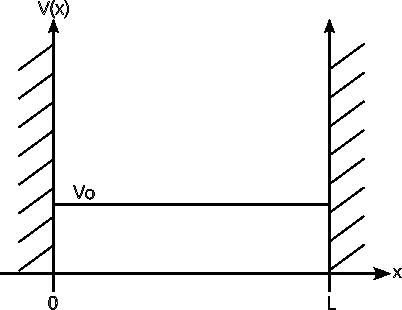
\includegraphics[width=0.5\textwidth]{path469.pdf}
\end{figure}
\begin{align*}
	\tilde{H} & = \hat{H}_o + \lambda \hat{V}\\
	& = \frac{-\hbar^2}{2m}\frac{d^2}{dx^2} + V_o,\,\,\,x \in\,\text[0,L]
\end{align*}
\textbf{Schrodinger Equation}
\begin{equation*}
	\frac{-\hbar^2}{2m}\frac{d^2 \tilde{\psi}_n(x)}{dx^2} + \lambda \tilde{V}_o \tilde{\psi}_n(x) 
	= \tilde{E}_n \tilde{\psi}_n(x)
\end{equation*}
for the perturbated system.\\
\\
For the unperturbated system:
\begin{equation*}
	\hat{H}_o \psi_n = E_n \psi_n
\end{equation*}
(ODE):
\begin{equation*}
	\psi^{"}_n(x) = \frac{-2mE_n \psi_n(x)}{\hbar^2} \longrightarrow \psi_n (x) = A \cos\left( 
	\sqrt{\frac{2m E_n}{\hbar^2}}x\right) + B \sin\left( 
	\sqrt{\frac{2m E_n}{\hbar^2}}x\right) 
\end{equation*}
(B.C):
\begin{align*}
	\psi (0) & = \psi (L) = 0\\
	\psi(0) & = A \cancelto{1}{\cos(0)} + B \cancelto{0}{\sin(0)} + \Longrightarrow A = 0\\
	\psi(L) & = B \sin\left(\sqrt{\frac{2mE_n}{\hbar^2}L}\right) = 0 \Longrightarrow 
	\sqrt{\frac{2mE_n}{\hbar^2}L} = n\pi,\,\,\, n \in \mathbb{N}\,\,wlog
\end{align*}
\begin{equation*}
	\Longrightarrow E_n = \frac{n^2 \pi^2 \hbar^2}{2mL^2} \longleftarrow \text{Eigenenergies
		of the unperturbed infinite square well.}
\end{equation*}
\begin{equation*}
	\psi(x) = B \sin \left(\frac{\sqrt{2m}}{\hbar}\left(\frac{n^2 \pi^2 \hbar^2}{2mL^2} \right)^{1/2}
	x\right) = B \sin \left(\frac{n\pi x}{L} \right)
\end{equation*}
\subsection{Normalisation}
\begin{align*}
	\big<\psi_n\big|\psi_n \big> & = 1\\
	& = B^2 \int_{0}^{L}\sin^2 \left(\frac{n\pi x}{L}\right)dx\\
	& = B^2 \frac{L}{2} = 1\\
	\Longrightarrow B & = \sqrt{\frac{2}{L}}
\end{align*}
\begin{align*}
	\psi_n (x) & = \sqrt{\frac{2}{L}} \sin \left(\frac{n\pi x}{L} \right),\,\,\,E_n = \frac{n^2 \pi^2
	\hbar^2}{2mL^2}\\
		\hat{E}_n & = E_n + \big<\psi_n\big|\hat{V}\big|\psi_n\big> + \sum_{n'\neq n} 
		\frac{\big|\big<\psi_{n'}\big|\hat{V}\big|\psi_n\big>\big|^2}{E_n - E_{n'}}
\end{align*}
\begin{equation*}
	\tilde{E}_n = \frac{n^2 \pi^2 \hbar^2}{2mL^2} +\int_{0}^{L} \frac{2}{L} \cancelto{1}{\sin^2 
		\left(\frac{n \pi x}{L} \right)}.V_o dx + \sum_{n\neq n'} \frac{\bigg|\cancelto{0}{\int_{0}^{L} \sin 
	\left(\frac{n\pi x}{L}\right)} \sin \left(\frac{n, \pi x}{L}\right)dx \bigg|^2}{n^2 - n'^2} V^2_o 
	\frac{2m L^2}{\pi^2 \hbar^2}
\end{equation*}
\begin{equation*}
	\boxed{\tilde{E}_n  = \frac{n^2 \pi^2 \hbar^2}{2mL} + V_o }
\end{equation*}
Basically, if we add a constant potential $V_o$ everywhere, this just shifts the eigenenergies 
by $V_o$. \\
\\
The $2^{nd}$ order term is zero because $V_o$ does not alter the wavefunction $\psi_n$ and 
$\big<\psi_{n'}\big|\psi_n \big > = \delta_{n'n}$.\\
\\
If we half the potential, the eigenenergies will be shifted by $V_o/2$.
\begin{multline*}
	E_n = \frac{n^2 \pi^2 \hbar^2}{2mL} + \int_{0}^{\frac{L}{2}} V_o \sin^2 \left(\frac{n\pi x}
	{L}\right)\frac{2}{L} dx\\
	+ \sum_{n\neq n'} \frac{V^2_o}{n^2 - n'^2} \frac{2mL^2}{\pi^2 \hbar^2}\bigg|\int_{0}^{\frac{L}{2}}
	\sin\left(\frac{n\pi x}{L}\right)\sin\left(\frac{n'\pi x}{L}\right)dx \bigg|^2
	\left(\frac{2}{L}\right)^2
\end{multline*}
\begin{multline*}
	E_n = \frac{n^2 \pi^2 \hbar^2}{2mL} +V_o \frac{2}{L} \left(\frac{L}{2\cdot 2}\right) + \frac{2mL^2}
	{\pi^2 \hbar^2}V_o^2 \sum_{n'\neq n} \frac{1}{n^2 - n'^2}\cdot \bigg| \frac{1}{2}\int_{0}^
	{\frac{L}{2}} \cos \left(\frac{(n-n')\pi x}{L}\right)\\
	+ \cos \left(\frac{(n+n')\pi x}{L}\right)dx \bigg|^2\cdot \left(\frac{2}{L}\right)^2
\end{multline*}
\begin{multline*}
	E_n = \frac{n^2 \pi^2 \hbar^2}{2mL} + \frac{V_o}{2} + \frac{2mL^2 V^2_o}{\pi^2 \hbar^2}\sum_{n'\neq n}
	\frac{1}{n^2 - n'^2}\frac{1}{4}\cdot \Bigg|\frac{L}{\pi}\left(\frac{\sin\left(\frac{(n-n')x\pi}{L}\right)}
	{n-n'}\right)\\
	-\left(\frac{\sin\left(\frac{(n+n')x\pi}{L}\right)}{n+n'}\right)\Bigg|_{0}^{\frac{L}{2}}\Bigg|^2
\left(\frac{2}{L}\right)^2
\end{multline*}
\begin{equation*}
 E_n = \frac{n^2 \pi^2 \hbar^2}{2mL} + \frac{V_o}{2} + \frac{2mL^2 V^2_o}{\pi^2 \hbar^2}\sum_{n'\neq n}
 \frac{1}{n^2-n'^2}\Bigg|\frac{\sin((n-n')\pi/2)}{n-n'} +\frac{\sin((n+n')\pi/2)}{n+n'}\Bigg|^2
\end{equation*}
\begin{multline*}
 E_n = \frac{n^2 \pi^2 \hbar^2}{2mL} +\frac{V_o}{2} + \frac{2mL^2 V^2_o}{\pi^2 \hbar^2}\sum_{n'\neq n}
 \frac{1}{(n-n')(n+n')}\Bigg|\frac{(1-(-1)^{n-n'})}{2}\frac{(-1)^{\frac{n-n'-1}{2}}}{n-n'}\\
 + \frac{(1-(-1))^{n+n'}(-1)^{\frac{n+n'}{2}}}{n+n'} \Bigg|^2
\end{multline*}
\textbf{If $n+n,$ is even, then $n-n,$ is even.}\\
Proof:
\begin{align*}
	n+n' & = 2k\\
	n-n' & = n+n' -2n'=2k -2n'\,\,\Longrightarrow\text{Which is even.}
\end{align*}
\textbf{If $n+n,$ is odd, then $n-n,$ is odd.}\\
Proof:
\begin{align*}
	n+n' & = 2k + 1\\
	n-n' & = n+n'-2n' = 2k+1-2n'\\
	& = 2(k - n') + 1\,\,\Longrightarrow \text{is odd.}
\end{align*}
Then:
\begin{equation*}
	\frac{1-(-1)^{n-n'}}{2} = \frac{1-(-1)^{n+n'}}{2}
\end{equation*}
\begin{align*}
	\tilde{E}^{(2)}_n & = \frac{2mL^2V_o^2}{\pi^4 \hbar^2}\sum_{n'\neq n}\frac{1}{(n-n')(n+n')}\bigg|
	\frac{1-(-1)^{n+n'}}{2} \bigg|\bigg|\frac{(-1)^{\frac{n-n'-1}{2}}}{n-n'} + \frac{(-1)^{\frac{n+n'}
{2}}}{n+n'} \bigg|^2
\end{align*}
Only when $n+n'$ is odd we have a correction.
\begin{align*}
	\tilde{E}^{(2)}_n & = \frac{2mL^2V_o^2}{\pi^4 \hbar^2}\sum_{n'\neq n}\frac{1}{(n-n')(n+n')}\bigg|
	\frac{1-(-1)^{n+n'}}{2} \bigg|\bigg|(-1)^{\frac{n+n'}{2}}\bigg|^2\bigg|\frac{1}{n+n'} - 
	\frac{1}{n-n'}\bigg|^2\\
	& =\frac{2mL^2V_o^2}{\pi^4 \hbar^2}\sum_{n'\neq n}\frac{1}{(n-n')(n+n')}\left(
	\frac{1-(-1)^{n+n'}}{2}\right) \Bigg|\frac{n-n'-(n+n')}{(n+n')(n-n')}\Bigg|^2\\
	& = \frac{8mL^2V_o^2}{\pi^4 \hbar^2}\sum_{n'\neq n} \frac{n'^2}{(n^2 - n'^2)^3}\frac{1-(-1)^{n+n'}
	}{2}
\end{align*}
We only have a 2nd order correction when we go odd $\rightarrow$ even or even $\rightarrow$ odd.\\
\\
\textbf{Suppose n is even:}\\
\begin{align*}
	n = 2k \Longrightarrow \Psi_{2k}\left(\frac{L}{2}\right) & = 0\\
	\Psi_{2k + 1} \left(\frac{L}{2}\right) & = \pm \sqrt{\frac{2}{L}}
\end{align*}
%%%%%%%%%%%%%%%%%%%%%%%%%%%%%%%%%%%%%%%%%%%%%%%%%%%%%%%%%%%%%%%%%%%%%%%%%%%%%%%%%%%%%%%%%%%%%%%%%%
%%%%%%%%%%%%%%%%%%%%%%%%%%%%%%%%%%%%%%%%%%%%%%%%%%%%%%%%%%%%%%%%%%%%%%%%%%%%%%%%%%%%%%%%%%%%%%%%%%
%%%%%%%%%%%%%%%%%%%%%%%%%%%%%%%%%%%%%%%%%%%%%%%%%%%%%%%%%%%%%%%%%%%%%%%%%%%%%%%%%%%%%%%%%%%%%%%%%%
\subsection{Example: 1D Infinite Square Well Potential + Perturbative Potential $V(x) = \alpha 
\delta(x-\frac{L}{2})$.}
\begin{figure}[h]
  \centering
	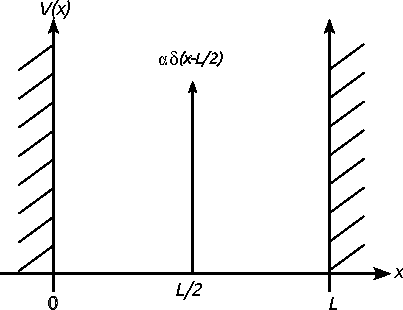
\includegraphics[width=0.5\textwidth]{delta.pdf}
\end{figure}
Criteria for using the perturbation theory:
\begin{equation*}
	\big|\big<\psi_{n'}\big|\hat{V}\big|\psi_n\big>\big|^2 \ll (E_n - E_{n'})^2
\end{equation*}
\begin{equation*}
	\psi_n = \sqrt{\frac{2}{L}} \sin \left(\frac{n\pi x}{L}\right),\,\,\,\,\,\,\,\,\,\,\,\,\,\,\,\,\,
	E_n = \frac{n^2 \pi^2 \hbar^2}{2mL^2}
\end{equation*}
\begin{align*}
	\big|\big<\psi_{n'}\big|\hat{V}\big|\psi_n\big>\big|^2 & = \Bigg |\alpha\int_{0}^{L}\frac{2}{L}
	\sin\left(\frac{n'\pi x}{L}\right) 	\sin\left(\frac{n\pi x}{L}\right) \delta \left(x - 
	\frac{L}{2}\right)dx\Bigg|^2\\
	& = \frac{4}{L^2}\alpha^2 	\sin^2\left(\frac{n'\pi}{L}\right)\sin^2\left(\frac{n\pi}{L}\right)\\
	& = \left(\frac{2\alpha}{L}\right)^2 \underbrace{\left(\frac{1-(-1)^{n'}}{2}\right)}_\text{n' is
	odd}\underbrace{\left(\frac{1-(-1)^{n}}{2}\right)}_\text{n is odd}
\end{align*}
\begin{equation*}
	(E_n-E_{n'})^2 = \left(\frac{\pi^2 \hbar^2}{2mL^2}\right)(n^2 - n'^2)^2
\end{equation*}
\begin{equation*}
	\frac{4\alpha^2}{L^2} \ll \frac{\pi^4 \hbar^4}{4m^2L^4}(n-n')^2(n+n')^2
\end{equation*}
\begin{equation*}
	\alpha \ll \frac{\pi^2 \hbar^2}{2mL}\big|n^2 - n'^2\big| = \frac{\pi^2 - n'^2}{2mL}
	\underbrace{(n-n')}_{\geq 2}\underbrace{(n+n')}_{\geq 4}
\end{equation*}
\begin{equation*}
	\alpha << \frac{4 \pi^2 \hbar^2}{mL}
\end{equation*}
\begin{align*}
	\tilde{E}^{(1)}_n & = \big<\psi_n \big| \hat{V}\big|\psi_{n}\big>\\
	& = \int_{2}^{L} \frac{2}{L} \sin^2 \left(\frac{n\pi x}{L}\right)\alpha\delta\left(x - \frac{L}{2}
	\right)dx\\
	& = \frac{2}{L}\sin^2 \left(\frac{n\pi L}{2L}\right)\cdot \alpha \cancelto{0}{\int_{0}^{L}
	\delta\left(x - \frac{L}{2}\right)}\\
	& = \frac{2}{L}\left(\frac{1-(-1)^n}{2}\right)
\end{align*}
\begin{equation*}
	\tilde{E}_{2k} = \frac{\pi^2 \hbar^2 (2k)^2}{2mL^2} + 0
\end{equation*}
when $\psi_{2k}$ has no $1^{st}$ order correction to their eigenenergies.
\begin{equation*}
	\tilde{E}_{2k-1} = \frac{\pi^2 \hbar^2 (2k-1)^2}{2mL^2} + \frac{2\alpha}{L}
\end{equation*}
odd $\psi_{2k-1}$ have a constant shift by $\frac{2}{L}\alpha$.
\begin{equation*}
	\psi_{2k}\left(\frac{L}{2}\right) = \sqrt{\frac{2}{L}} \sin\left(\frac{2k\pi L}{2L}\right) = 
	\sqrt{\frac{2}{L}}\sin(\pi k)= 0
\end{equation*}
even $n$ index wavefunctions all have a node @ $\frac{L}{2}\rightarrow \left(
\psi_{2k}\left(\frac{L}{2}\right)=0\right)$.\\
\\
Since $V(x) = \alpha \delta\left(x - \frac{2}{L}\right)$ is non-zero only @ $\frac{L}{2}$ it does nothing to the even
n wavefunctions.\\
\\
$\because$ a particle in the $2k-1$, odd n, state $\psi_{2k-1}$ has a probability $\Big|\psi_{2k-1}
\left(\frac{L}{2}\right)\Big|^2 = \frac{2}{L}$ of being @ $\frac{L}{2}$.
\newpage
%%%%%%%%%%%%%%%%%%%%%%%%%%%%%%%%%%%%%%%%%%%%%%%%%%%%%%%%%%%%%%%%%%%%%%%%%%%%%%%%%%%%%%%%%%%%%%%%%%%
%%%%%%%%%%%%%%%%%%%%%%%%%%%%%%%%%%%%%%%%%%%%%%%%%%%%%%%%%%%%%%%%%%%%%%%%%%%%%%%%%%%%%%%%%%%%%%%%%%%
%%%%%%%%%%%%%%%%%%%%%%%%%%%%%%%%%%%%%%%%%%%%%%%%%%%%%%%%%%%%%%%%%%%%%%%%%%%%%%%%%%%%%%%%%%%%%%%%%%%
%%%%%%%%%%%%%%%%%%%%%%%%%%%%%%%%%%%%%%%%%%%%%%%%%%%%%%%%%%%%%%%%%%%%%%%%%%%%%%%%%%%%%%%%%%%%%%%%%%%
\section{Lecture 4}
May 02, 2023
\subsection{Example: Harmonic Oscillator}
\begin{figure}[h]
  \centering
	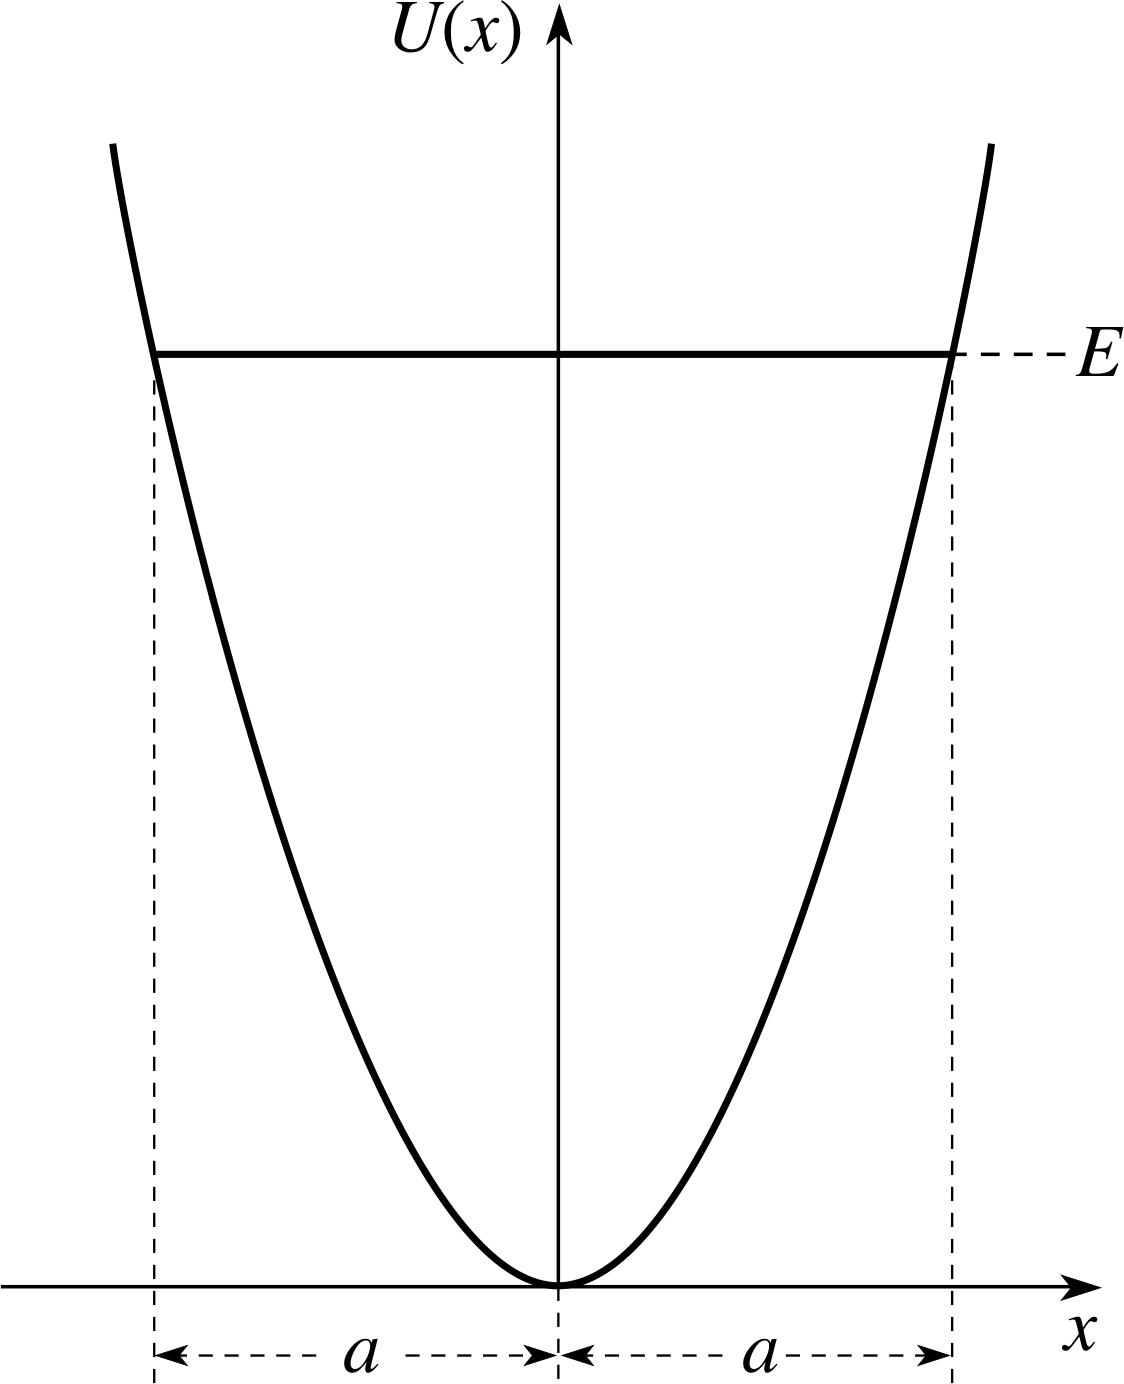
\includegraphics[width=0.4\textwidth]{HO.png}
\end{figure}
\begin{equation*}
	V(x) = kx^2 = \omega^2 m x^2,\,\,\,\,\,\,\omega = \sqrt{\frac{k}{m}}:\,\text{The frequency of
	oscillation}
\end{equation*}
\textbf{Hamiltonian for the Harmonic Oscillator:}
\begin{equation*}
	\hat{H}_o =\underbrace{\frac{-\hbar^2}{2m}\frac{d^2}{dx^2}}_{K.E} + \underbrace{\omega^2 m x^2}_
	{P.E = \hat{V}}
\end{equation*}
\textbf{Eigenenergies}
\begin{equation*}
	E_n = \hbar\omega\left(n + \frac{1}{2}\right)
\end{equation*}
$x^2$ can be written in terms of rising and lowering operators $\hat{a}_+ + \hat{a}_-$, respectively
as:
\begin{equation*}
	\hat{x} =	C \left(\hat{a}_+ + \hat{a}_-\right)
\end{equation*}
where if $\big|n\big>$ are the eigenstates of the SHO:\\
\\
\textbf{Rising operator}
\begin{equation*}
	\hat{a}_+ \big|n\big> = \sqrt{n +1}\big|n+1\big>
\end{equation*}
\textbf{Lowering operator}
\begin{equation*}
	\hat{a}_- \big|n\big> = \sqrt{n}\big|n-1\big>
\end{equation*}

\begin{equation*}
	\big<n\big|\hat{H}_o\big|n\big> = \big<n\big|\hat{T}\big|n\big> + 
  \underbrace{\big<n\big|\hat{V}\big|n\big>}_{\mathclap{\text{the eigenenergy }E_n}}
\end{equation*}
The particle has zero average K.E, 1/2 time to the left, and 1/2 time to the right.\\
\\
Then,
\begin{equation*}
	\big<n\big|\omega^2 m x^2\big|n\big> = \hbar \omega\left(n + \frac{1}{2}\right) = E_n
\end{equation*}
\textbf{but what is C?}
\begin{align*}
	\hbar \omega\left(n + \frac{1}{2}\right) & = \omega^2 m\big<n\big|C^2 \left(\hat{a}_+ + \hat{a}_-\right)
	\left(\hat{a}_+ + \hat{a}_-\right)\big|n\big>\\
	& = C^2 \omega^2 m\cdot\big<n\big|\hat{a}_+ \hat{a}_+ + \hat{a}_+ \hat{a}_- +  \hat{a}_- \hat{a}_+ +
	\hat{a}_-\hat{a}_-\big|n\big>\\
	& = C^2 \omega^2 m\left(\big<n\big|\sqrt{n+2}\sqrt{n+1}\big|n+2\big> + \big<n\big|n\big>n
	+ (n+1)\big<n\big|n\big>+ \big<n\big|n-2\big>\sqrt{n-1}\sqrt{n}\right)\\
	& = C^2 \omega^2 m\left(\sqrt{n+2}\sqrt{n+1}\cdot\cancelto{0}{\delta_{n,n+2}}
	+ (2n+1)\cdot\cancelto{1}{\delta_{n,n}}+\sqrt{n-1}\sqrt{n}\cdot\cancelto{0}{\delta_{n,n-2}}\right)\\
	& =  C^2 \omega^2 m\cdot (2n+1)
\end{align*}
\begin{equation*}
	C^2 = \frac{\hbar \omega\left(n+\frac{1}{2}\right)}{\omega^2 m (2n+1)} \Rightarrow C =
	\sqrt{\frac{\hbar}{2\omega m}}
\end{equation*}
Thus, 
\begin{equation*}
	\hat{x} = \sqrt{\frac{\hbar}{2\omega m}}\left(\hat{a}_+ \hat{a}_-\right)
\end{equation*}
\begin{equation*}
	\big<n\big| \hat{a}_- \hat{a}_+\big|n\big> = n+1\,\,\,\,\text{and}\,\,\,\,
	\big<n\big| \hat{a}_+ \hat{a}_-\big|n\big> = n
\end{equation*}
\begin{equation*}
	\hat{a}_+\big|n\big> = \sqrt{n+1}\big|n+1\big>\,\,\,\,\text{and}\,\,\,\,\hat{a}_- \big|n\big> = 
	\sqrt{n}\big|n-1\big>
\end{equation*}
\\
Let $\big|n\big>$ be the $n^{th}$ eigenstate of the SHO with eigenenergy $E_n = 
\hbar\omega\left(n + \frac{1}{2}\right) $.\\
\\
\textbf{Perturbation}\\
\\
Suppose we increase the spring constant $k$ to $k + \epsilon$ where $\epsilon << 1$, e.g. reduce 
the temperature.\\
\\
\textbf{What are the "new" perturbed eigenenergies?}
\begin{align*}
	E_n & = \hbar\sqrt{\frac{k}{m}}\left(n+\frac{1}{2}\right)\\
	\tilde{E}_n	& =\hbar\sqrt{\frac{k}{m}}\left(n+\frac{1}{2}\right)\cdot\sqrt{1+\epsilon}\\
							& = E_n\cdot \sqrt{1+\epsilon} \approx E_n\cdot\left(1+\frac{\epsilon}{2}
							-\frac{\epsilon^2}{8}+\frac{\epsilon^3}{16}\right)
\end{align*}
expanding using the Tylor series. \\
\\
\textbf{Applying T.I.N.D.P.T}\\
\\
The perturbed hamiltonian is:
\begin{equation*}
	\tilde{H} = \frac{-\hbar}{2m}\frac{d^2}{dx^2}+k\hat{x}^2+k\epsilon\hat{x}^2
\end{equation*}
, so, our perturbation is $\hat{V} = k\epsilon\hat{x}^2$.
\begin{equation*}
	\tilde{E}_n = E_n+\big<n\big|\hat{V'}\big|n\big>+\sum_{n'\neq n}\frac{\big|\big<
	n'\big|\hat{V}'\big|n\big>\big|^2}{E_n - E_{n'}}
\end{equation*}
where:\\
\\
$E_n$: Unperturbed eigenenergy.\\
\\
$E_n - E_{n'} $: Energy difference between $\big|n\big>$ and $\big|n'\big>$.\\
\\
$ \big|\big<n'\big|\hat{V}'\big|n\big>\big|^2$: Probability of $\big|n\big>\rightarrow\big|n'\big>
\rightarrow\big|n\big>$ under the action of $\hat{V}$. Note that $\{\big|n\big>\}$ are not usually 
eigenstates of $\hat{V}'$.\\
\\
\textbf{Note:}
\begin{equation*}
	\big|\big<n'\big|\hat{V}'\big|n\big>\big|^2	\lll \big|E_n - E_{n'}\big|^2,\,\forall n'\neq n
\end{equation*}
for TINDPT to apply to $\tilde{E}_n$.\\
\\
\textbf{Remember:} If we need to go to $3^{RD}$ order, TINDPT does not apply unless both $1^{ST}$
and $2^{ND}$ order terms are zero, in which case the $3^{RD}$ order term probably is zero as well.\\
\\
If $E_{n'}>E_n \Longrightarrow E_n - E_{n'}<0$\\
\\
If $E_{n'}<E_n \Longrightarrow E_n - E_{n'}>0$\\
\\
The second order correction to the energy,
\begin{equation*}
	\sum_{n'\neq n}\frac{\big|\big<
	n'\big|\hat{V}'\big|n\big>\big|^2}{E_n - E_{n'}}
\end{equation*}
has positive terms for states below $E_n$, and negative terms for states above $E_n$. This is known
as \textbf{level repulsion.}
\begin{figure}[H]
  \centering
	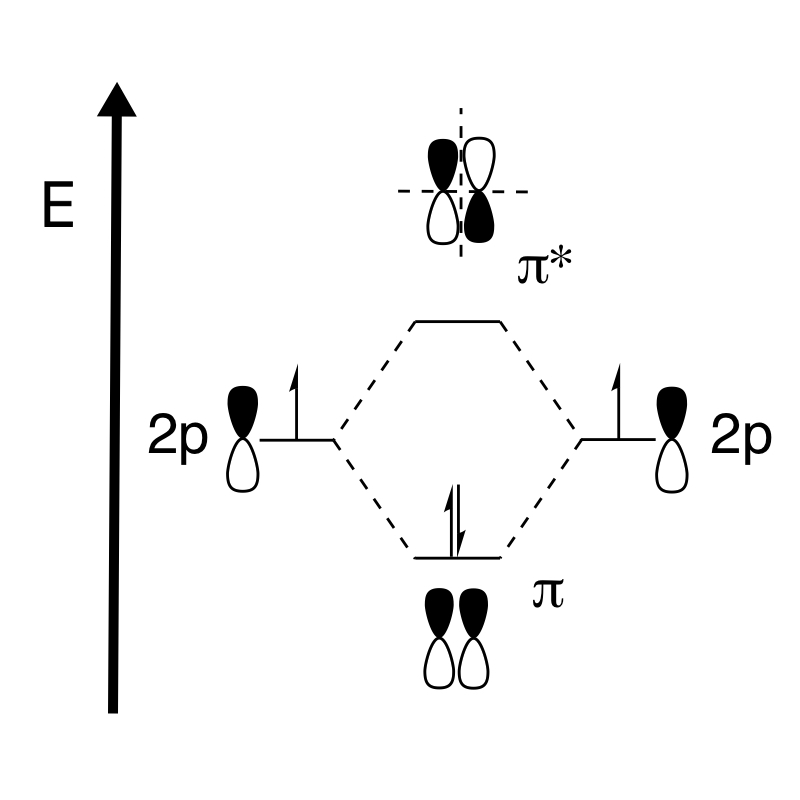
\includegraphics[width=0.35\textwidth]{repulsion.jpg}
\end{figure}
\begin{itemize}
	\item Same phase: bonding orbital.
	\item Opposite phase: antibonding orbital.
	\end{itemize}
Hint: Levels repell each other.
\begin{equation*}
	\tilde{E}_n = \hbar\omega\left(n+\frac{1}{2}\right)+\frac{\epsilon}{2}E_n
\end{equation*}
\begin{align*}
	\big<n\big|\hat{V}'\big|n\big> = \Bigg<n\Bigg|\frac{k\epsilon}{2}\hat{x}^2\Bigg|n\Bigg>
	& = \frac{m\omega^2}{2}\frac{\epsilon \hbar}{2m}\big<n\big|(\hat{a}_+\hat{a}_-)^2\big|n\big>\\
	& = \frac{\epsilon\hbar\omega}{2}\frac{(2n+1)}{2} = \frac{\epsilon}{2}\hbar\omega\left(n+\frac{1}{2}\right)\\
	& = \frac{\epsilon}{2}E_n
\end{align*}
\textbf{Virial Theorem}
\begin{equation*}
	\big<\hat{T}\big> = \big<\hat{V}\big>
\end{equation*}
\textbf{Schrodinger Equation:}
\begin{equation*}
	\big<\hat{T}\big>+\big<\hat{V}\big> = E_n \Longrightarrow \big<\hat{V}\big> = \frac{1}{2}E_n
\end{equation*}
\begin{equation*}
	\hat{V} = \frac{1}{2}kx^2 = \frac{1}{2}m\omega^2x^2
\end{equation*}
\subsection{$2^{nd}$ Order Correction}
\begin{align*}
	\tilde{E}^{2}_n & = \sum_{n'\neq n}\frac{\big|\big<n'\big|\hat{V}'\big|n\big>\big|^2}
	{E_n - E_{n'}}= \sum_{n'\neq n}\frac{\big|\big<n'\big|\frac{\epsilon}{2}kx^2\big|n\big>\big|^2}
	{\hbar\omega\left(n+\frac{1}{2}\right) - \hbar\omega\left(n'+\frac{1}{2}\right)}\\
	& = \frac{\epsilon^2}{4}\frac{m^2\omega^4}{\hbar\omega}\left(\frac{\hbar}{2m\omega}\right)^2
	\sum_{n'\neq n}\frac{1}{n-n'}\Big| \big<n\big|\hat{a}_+ \hat{a}_+ + \hat{a}_+ \hat{a}_- + 
	\hat{a}_- \hat{a}_+ +\hat{a}_-\hat{a}_-\big|n\big>\Big|^2\\
	& = \frac{\epsilon^2}{4}\hbar\omega \sum_{n'\neq n}\frac{1}{n-n'}\Big|
		\sqrt{n+2}\sqrt{n+1}\big<n'\big|n+2\big> + \big<n'\big|n\big>n
	+ (n+1)\big<n\big|n'\big>\\
  & + \big<n'\big|n-2\big>\sqrt{n-1}\sqrt{n}\Big|^2\\
	& = \frac{\epsilon^2}{16}\hbar\omega\sum_{n'\neq n}\frac{1}{n-n'}\Big|\sqrt{n+1}\sqrt{n+2}
	\cdot\delta_{n',n+2}+ (2n+1)\cdot\cancelto{0}{\delta_{n'n}}+ \sqrt{n}\sqrt{n-1}\cdot
	\delta_{n',n-2}\Big|^2\\
	& = \frac{\epsilon^2}{16}\hbar\omega\sum_{n'\neq n}\frac{1}{n-n'}\Big|(n+1)(n+2)\cdot\delta^2
	_{n', n+2} + 2\sqrt{n}\sqrt{n+2}\sqrt{n+1}\sqrt{n-1}\cdot\cancelto{0}{\delta_{n',n+2}
	\delta_{n',n-2}}\\
  & +n(n+2)\delta^2_{n',n-2}\Big|^2
\end{align*}
Note that $n'$ can't equal $n+2$ and $n-2$ at the same time, that is why the delta functions 
cancel.
\newpage
%%%%%%%%%%%%%%%%%%%%%%%%%%%%%%%%%%%%%%%%%%%%%%%%%%%%%%%%%%%%%%%%%%%%%%%%%%%%%%%%%%%%%%%%%%%%%%%%%%
%%%%%%%%%%%%%%%%%%%%%%%%%%%%%%%%%%%%%%%%%%%%%%%%%%%%%%%%%%%%%%%%%%%%%%%%%%%%%%%%%%%%%%%%%%%%%%%%%%
%%%%%%%%%%%%%%%%%%%%%%%%%%%%%%%%%%%%%%%%%%%%%%%%%%%%%%%%%%%%%%%%%%%%%%%%%%%%%%%%%%%%%%%%%%%%%%%%%%
\section{Lecture 5}
May 03, 2023
\subsection{Example: SHO}
$k \longrightarrow (1+\epsilon)k$
\begin{equation*}
	E_n = \hbar\omega \left(n+\frac{1}{2}\right)
\end{equation*}
$$\omega = \sqrt{\frac{k}{m}},\,\,\,\,\hat{V}= \frac{1}{2}kx^2$$
\textbf{Exact Solution}
\begin{align*}
	\tilde{E}_n &= \hbar\sqrt{\frac{k(1+\epsilon)}{m}}\left(n+\frac{1}{2}\right)\\
	&= \hbar\omega\left(n+\frac{1}{2}\right)\sqrt{1+\epsilon}\\
	&= E_n\sqrt{1+\epsilon}
\end{align*}
\begin{equation*}
	\boxed{\tilde{E_n} \approx E_n\left(1+\frac{\epsilon}{2}- \frac{\epsilon^2}{8}
	+\mathcal{O}(\epsilon^3)\right)}
\end{equation*}
\textbf{Perturbation Theory}
\begin{equation*}
	\tilde{E}_n = E_n+\big<n\big|\hat{V}\big|n\big>+\sum_{n'\neq n}\frac{\big|\big<n'\big|\hat{V}
	\big|n\big>\big|^2}{E_n-E_{n'}}
\end{equation*}
Level repulsion scales the energy.
\begin{equation*}
	\big|\tilde{n}\big> = \big|n\big> \sum_{n'\neq n}\frac{\big<n'\big|\hat{V}\big|n\big>}{E_n-E_{n'}}
	\big|n'\big>
\end{equation*}
In general, the appropiate wavefunctions from TINDPT are not very accurate.
\begin{equation*}
	\tilde{E}_n = \hbar\omega\left(n+\frac{1}{2}\right)+\big<n\big|\frac{\epsilon}{2}kx^2\big|n\big>
	+ \sum_{n'\neq n} \frac{\big|\big<n'\big|\frac{\epsilon}{2}kx^2\big|n\big>\big|^2}{E_n-E_{n'}}
\end{equation*}
\begin{equation*}
	\big<n\big|\frac{\epsilon}{2}kx^2\big|n\big> = \frac{m\omega^2}{2}\frac{\hbar\epsilon}{2m\omega}
	\big| \big<n\big|\hat{a}_+ \hat{a}_+ + \hat{a}_+ \hat{a}_- + 
	\hat{a}_- \hat{a}_+ +\hat{a}_-\hat{a}_-\big|n\big>\big|^2
\end{equation*}
But,
\begin{equation*}
	\hat{x}\equiv \sqrt{\frac{\hbar}{2m\omega}}\left(\hat{a}_+ + \hat{a}_-\right),\,\,\,\,\,\,
	\hat{a}_+\big|n\big> = \sqrt{n+1}\big|n+1\big>,\,\,\,\,\,\,\hat{a}_-\big|n\big>=\sqrt{n}\big|n-1\big>
\end{equation*}
Then
\begin{equation*}
	\big<n\big|\hat{V}\big|n\big> = \frac{\epsilon}{4}\hbar\omega\left(n+n+1\right) = \frac{\epsilon}
{2}\hbar\omega\left(n+\frac{1}{2}\right) = \boxed{\frac{\epsilon}{2}E_n}
\end{equation*}
Now, let's compute the second order correction:
\begin{align*}
	\tilde{E}_n^{(2)} &= \left(\frac{\epsilon}{2}m\omega^2\right)^2 \left(\frac{\hbar}{2m\omega}\right)^2
	\frac{1}{\hbar\omega}\sum_{n'\neq n}\frac{\big|\big<n'\big|\hat{a}_+ \hat{a}_+ + \hat{a}_+
	\hat{a}_- + \hat{a}_- \hat{a}_+ +\hat{a}_-\hat{a}_-\big|n\big>\big|^2}{n+\frac{1}{2} - 
	\left(n+\frac{1}{2}\right)}\\
	&= \frac{\epsilon^2}{16}\hbar\omega\sum_{n'\neq n}\big|\sqrt{n+2}\sqrt{n+1}\underbrace{\big<n'
	\big|n+2\big>}_{\delta_{n',n+2}} + \sqrt{n-1}\sqrt{n}\underbrace{\big<n'\big|n-2\big>}
	_{\delta_{n',n-2}}\big|^2\\
	&= \frac{\epsilon^2}{16}\hbar\omega\left(\sum_{n'\neq n} \frac{(n+2)(n+1)
	\delta_{n',n+2}}{n-(n-2)}+\frac{(n-1)n\cdot\delta_{n',n-2}}{n-(n-2)}\right)\\
	&= \frac{\epsilon^2}{16}\hbar\omega\left(\frac{n^2-n-n^2-2n-n-2}{|2|}\right)\\
	&= \frac{\epsilon^2 \hbar\omega}{16}\left(\frac{-4n-2}{2}\right)^{1/2}
\end{align*}
\begin{equation*}
	\boxed{\tilde{E}_n^{(2)} = \frac{-\epsilon^2\hbar\omega}{8}\left(n+\frac{1}{2}\right)}
\end{equation*}
Then,
\begin{equation*}
	\tilde{E} = E_n\left(1+\frac{\epsilon}{2}-\frac{\epsilon^2}{8}\right)
	= E_n\sqrt{1+\epsilon}\,\,\,\,\text{to}\,\,\,\,\mathcal{O}(\epsilon^3)
\end{equation*}
%%%%%%%%%%%%%%%%%%%%%%%%%%%%%%%%%%%%%%%%%%%%%%%%%%%%%%%%%%%%%%%%%%%%%%%%%%%%%%%%%%%%%%%%%%%%%%%%%%%
%%%%%%%%%%%%%%%%%%%%%%%%%%%%%%%%%%%%%%%%%%%%%%%%%%%%%%%%%%%%%%%%%%%%%%%%%%%%%%%%%%%%%%%%%%%%%%%%%%%
\subsection{Example: Interacting Bosons}
Consider two bosons which interact weakly in an infinite square well potential of width $L$ which 
weakly interact via $V(x_1,x_2)=-LV_o\delta(x_1 - x_2)$ where $V_o$ is a constant with dimensions 
of energy, $\delta$ is the Dirac delta function and $x_1$ and $x_2$ are the positions of the 
$1^{st}$ and $2^{nd}$ boson.\\
\textbf{Recall:} the dimension of the Dirac $\delta$-function is the inverse of its arguments so that:
\begin{equation*}
	\int_{-\infty}^{\infty} \delta(x)dx=1\,\,\,\,\,\text{(dimensionless)}
\end{equation*}
So, $\delta(x_1-x_2)$ has units of 1/Lenght, this is why we have a factor of $L$ in the def'n of 
$V(x_1, x_2)$.\\
\\
\textbf{Note:} $V(x_1,x_2)\longrightarrow \infty$ as $x_1 \longrightarrow x_2$, but so does the 
Coulomb interaction. Moreover, it is the expectation of the potential which is important and this 
will go as $V_o$, i.e. $\big<n\big|V\big|n\big>\sim V_o$ , when $x_1\neq x_2$, $V(x_1,x_2)=0$, so 
the two particles only interact when they reach or occupy the same point in space.
\begin{itemize}
	\item Bosons: many bosons can occupy the same state (spin 0).
	\item Fermions: Only one fermion can occupy the same state (spin $\frac{1}{2}$)
\end{itemize}
\textbf{Bosons:}
\begin{equation*}
	\Psi(x_1, x_2) = \Psi_a(x_1)\Psi_b(x_2) + \Psi_a(x_2)\Psi_b(x_1)
\end{equation*}
\begin{equation*}
	\Psi(x_1,x_2) = \Psi(x_1)\Psi(x_2)\,\,\,\,\text{Bosons are symmetric under exchange.}
\end{equation*}
\textbf{Fermions:}
\begin{equation*}
	\Psi(x_1, x_2) = \Psi_a(x_1)\Psi_b(x_2) + \Psi_a(x_2)\Psi_b(x_1)
\end{equation*}
\begin{equation*}
	\Psi(x_1, x_2) = -\Psi(x_2,x_1)\,\,\,\,\text{Fermions are antisymmetric under exchange.}
\end{equation*}
The n-particle wavefunction in terms of single particle wavefunctions can be written as a \textbf{
Slater Determinant}, i.e. the determinant of an $n\times n$ matrix of single particle wavefunctions
at positions $\chi$ to $\chi_n$.
\begin{figure}[H]
  \centering
	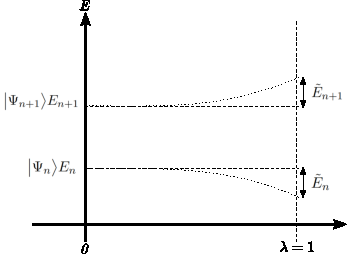
\includegraphics[width=0.6\textwidth]{shift.pdf}
\end{figure}
\begin{equation*}
	\tilde{H} = \underbrace{\hat{H}_o}_{E_n\big|\psi_n\big>} + \lambda\hat{V}
\end{equation*}
\begin{equation*}
	\tilde{\mathcal{E}}_n \approx \mathcal{E}_n+\big<n\big|\hat{V}\big|n\big> + 
	\sum_{n'\neq n} \frac{\big|\big<n'\big|\hat{V}\big|n\big>\big|^2}{\mathcal{E}_n-\mathcal{E}_{n'}}
\end{equation*}
\newpage
%%%%%%%%%%%%%%%%%%%%%%%%%%%%%%%%%%%%%%%%%%%%%%%%%%%%%%%%%%%%%%%%%%%%%%%%%%%%%%%%%%%%%%%%%%%%%%%%%
%%%%%%%%%%%%%%%%%%%%%%%%%%%%%%%%%%%%%%%%%%%%%%%%%%%%%%%%%%%%%%%%%%%%%%%%%%%%%%%%%%%%%%%%%%%%%%%%%
%%%%%%%%%%%%%%%%%%%%%%%%%%%%%%%%%%%%%%%%%%%%%%%%%%%%%%%%%%%%%%%%%%%%%%%%%%%%%%%%%%%%%%%%%%%%%%%%%
\section{Lecture 6}
May 08, 2023

\subsection{Example: two bosons in an infinite square well}
\begin{equation*}
	-LV_o\delta(x_1, x_2)
\end{equation*}
where, 
\begin{equation*}
V_o(x_1, x_2)=\begin{cases}
          0 \quad & 0 \leq x_1,\,\,x_2 \leq 1 \\
					\infty \quad & \text{Otherwise} \\
     \end{cases}
\end{equation*}
\textbf{For non-interacting bosons}\\
\\
Let $\Psi_{n_1, n_2}(x_1, x_2)$ be the two body wavefunction for the two bosons.\\
\\
\textbf{Schrodinger Equation:}
\begin{equation*}
	\hat{H}_o(x_1, x_2)\Psi(x_1, x_2) = E\Psi(x_1, x_2)
\end{equation*}
\begin{align*}
	\hat{H}_o(x_1, x_2) &= \hat{T}(x_1,x_2) + \hat{V}(x_1,x_2)\\
	&= \frac{-\hbar}{2m}\left(\frac{\partial^2}{\partial x_1^2}+\frac{\partial^2}{\partial x_2^2}\right)
	\Psi(x_1,x_2) = E\Psi(x_1,x_2)
\end{align*}
\begin{equation*}
	\boxed{\frac{\partial^2\Psi}{\partial x_1^2}+\frac{\partial^2\Psi}{\partial x_2^2} = 
\frac{-2mE}{\hbar^2}\Psi}
\end{equation*}
\\
Since the two particles are bosons, then the wavefunction is symmetric, i.e., 
\[\Psi(x_1,x_2) = \Psi(x_2,x_1)\]
\[\Psi_{n_1,n_2}(x_1,x_2)=\underbrace{\Psi_{n_1}(x_1)\Psi_{n_2}(x_2)}_\text{separable}+
\underbrace{\Psi_{n_1}(x_2)\Psi_{n_2}(x_1)}_\text{ensures symmetry}\]
\begin{multline*}
\Psi''_{n_1}(x_1)\Psi''_{n_2}(x_2) + \Psi_{n_1}(x_2)\Psi''_{n_2}(x_1) + 
\Psi_{n_1}(x_1)\Psi''_{n_2}(x_2)+ \Psi''+\Psi''_{n_1}(x_2)\Psi_{n_1}(x_1)\\
= \frac{-2mE}{\hbar^2}\left[\Psi_{n_1}(x_1)\Psi_{n_2}(x_2)+\Psi_{n_1}(x_2)\Psi_{n_2}(x_1)\right]
\end{multline*}
\\
\textbf{Separation of variables}

\begin{equation*}
	\Psi''_{n_1}(x_1)\Psi_{n_2}(x_2)+\Psi_{n_1}(x_1)\Psi''_{n_2}(x_2) 
	= \frac{-2mE}{\hbar^2}\Psi_{n_1}(x_1)\Psi_{n_2}(x_2)
\end{equation*}
\begin{equation*}
		\Psi_{n_1}(x_2)\Psi''_{n_2}(x_1)+\Psi''_{n_1}(x_2)\Psi_{n_1}(x_2) 
	= \frac{-2mE}{\hbar^2}\Psi_{n_1}(x_2)\Psi_{n_2}(x_1)
\end{equation*}
Divide (7.4) by $\Psi_{n_1}(x_1)\Psi_{n_2}(x_2)$ on both sides:
\begin{equation*}
	\frac{\Psi''_{n_1}(x_1)}{\Psi_{n_1}(x_1)}+\frac{\Psi''_{n_2}(x_2)}{\Psi_{n_2}(x_2)} 
	= \frac{-2mE}{\hbar^2}\longleftarrow\text{Eigenvalue}
\end{equation*}
\begin{equation*}
	\frac{\Psi''_{n_1}(x_1)}{\Psi_{n_1}(x_1)}= 
	\frac{-2mE}{\hbar^2}	-\frac{\Psi''_{n_2}(x_2)}{\Psi_{n_2}(x_2)} =
	-\lambda_{n_1}\longleftarrow\text{Eigenvalue}
\end{equation*}
then, 
\begin{equation*}
	\Psi''_{n_1}(x_1) = -\Psi_{n_1}(x_1)\lambda_{n_1}
\end{equation*}
\begin{equation*}
	\Longrightarrow \boxed{\mathlarger{\Psi}_{n_1}(x_1) = A \cos\left(\sqrt{\lambda_{n_1}} x_1\right)
	+ B \sin\left(\sqrt{\lambda_{n_1}} x_1\right)}
\end{equation*}
\begin{equation*}
	\mathlarger{\Psi}_{n_1}(0)=0 =A \quad \Psi_{n_1}(L) = 0 =B_1 \sin\left(\sqrt{\lambda_{n_1}}L\right)
\end{equation*}

\begin{equation*}
		\Longrightarrow \sqrt{\lambda_{n_1}}L = n_1 \pi
\Rightarrow\begin{cases}
	n_1 =0, \quad \text{no particle} \\
	\mathlarger{\Psi}_{n_1}(x_1)=-\mathlarger{\Psi}_{n_1}(x_1)\longrightarrow n_1 \in \mathbb{R}\\
     \end{cases}
\end{equation*}
Then, 
\begin{equation*}
	\mathlarger{\Psi}_{n_1}(x_1) = B_1 \sin{\left(\frac{n_1 \pi x}{L}\right)} \Longrightarrow \lambda_1 
	=\frac{n_1^2 \pi^2}{L^2}
\end{equation*}
\begin{equation*}
	\because \mathlarger{\Psi}_{n_2}(x_2) = B_2 \sin{\left(\frac{n_2 \pi x}{L}\right)} \Longrightarrow \lambda_2 
	=\frac{n_2^2 \pi^2}{L^2}
\end{equation*}
\begin{equation*}
	\Longrightarrow \frac{-2mE}{\hbar^2} = -\lambda_1 - \lambda_2 = \frac{-\pi^2}{L^2}
	\big(n_1^2-n_2^2\big)
\end{equation*}
\begin{equation*}
	\boxed{E_{n_1 n_2}= \frac{\pi^2 \hbar^2}{2mL^2}\left(n_1^2 + n_2^2\right)}
\end{equation*}
\\
\begin{equation*}
	\mathlarger{\Psi}_{n_1 n_2}(x_1,x_2) = \underbrace{B_1 B_2}_{A}\left(\sin{\left(\frac{n_1\pi x_1}{L}\right)}
	\sin{\left(\frac{n_2\pi x_2}{L}\right)}+\sin{\left(\frac{n_1\pi x_2}{L}\right)}
	\sin{\left(\frac{n_2\pi x_1}{L}\right)}\right)
\end{equation*}
We need to normalise the wave function, i.e. find $A$,
\begin{equation*}
	\big<\mathlarger{\Psi}_{n_1 n_2}(x_1, x_2)\big| \mathlarger{\Psi}_{n_1 n_2}(x_1, x_2)\big>=1
\end{equation*}
\begin{multline*}
	\Longrightarrow A^2 \int_{0}^{L}\int_{0}^{L}dx_1 dx_2\Bigg(\sin^2{\left(\frac{n_1\pi x_1}{L}\right)}
	\sin^2{\left(\frac{n_2\pi x_2}{L}\right)}+2\sin{\left(\frac{n_1\pi x_1}{L}\right)}
	\sin{\left(\frac{n_2\pi x_1}{L}\right)}\\
	\cdot\sin{\left(\frac{n_2\pi x_2}{L}\right)}\sin{\left(\frac{n_1\pi x_2}{L}\right)}+
	\sin^2{\left(\frac{n_1\pi x_2}{L}\right)}\sin^2{\left(\frac{n_2\pi x_1}{L}\right)}\Bigg)
\end{multline*}
\begin{equation*}
	=A^2\left(\frac{L}{2}\times\frac{L}{2}+2\frac{L}{2}\mathlarger{\delta}_{n_1 n_2}\times
	\mathlarger{\delta}_{n_1 n_2}+ \frac{L}{2}\times\frac{L}{2}\right) = A^2\frac{L^2}{4}
	2\left(1+\mathlarger{\delta}_{n_1 n_2}\right)
\end{equation*}
\[=A^2 \frac{L^2}{2}\left(1+\mathlarger{\delta}_{n_1 n_2}\right) \Longrightarrow 
\boxed{A = \frac{\sqrt{2}}{L}\frac{1}{\sqrt{1+\mathlarger{\delta{n_1 n_2}}}}}\]
Then, our normalised wavefunction is
\begin{equation*}
	\mathlarger{\Psi}_{n_1 n_2}(x_1, x_2) = \frac{\sqrt{2}}{L}\frac{1}{\sqrt{1+\mathlarger{\delta
	}_{n_1 n_2}}}\bigg(\sin{\left(\frac{n_1\pi x_1}{L}\right)}
	\sin{\left(\frac{n_2\pi x_2}{L}\right)}+\sin{\left(\frac{n_1\pi x_2}{L}\right)}
	\sin{\left(\frac{n_2\pi x_1}{L}\right)}\bigg)
\end{equation*}
and the eigenenergy
\begin{equation*}
	E_{n_1 n_2} = \frac{\pi^2 \hbar^2}{2mL^2}\left(n_1^2+n_2^2\right) = E_{n_1} + E_{n_2}
\end{equation*}
\subsubsection{Ground State}
\begin{equation*}
	E_{gs} = E_{11}=\frac{\pi^2 \hbar^2}{mL^2}
\end{equation*}
\begin{equation*}
	\mathlarger{\Psi}_{gs} = \frac{2}{L}\sin{\left(\frac{\pi x_1}{L}\sin{\left(\frac{\pi x_2}{L}
	\right)}\right)}
\end{equation*}

\subsubsection{1st Excited State}

\begin{equation*}
	E_{ex} = E_{12}=E_{21} = \frac{5 \pi^2 \hbar^2}{2mL^2} = 5E_1 = E_1+E_2
\end{equation*}
\begin{equation*}
	\mathlarger{\Psi}_{ex}=\frac{2}{L}\frac{\sin{\left(\frac{2\pi x_1}{L}\right)}
	\sin{\left(\frac{\pi x_2}{L}\right)}+\sin{\left(\frac{2\pi x_2}{L}\right)}
	\sin{\left(\frac{\pi x_1}{L}\right)}}{\sqrt{2}}
\end{equation*}

\subsubsection{Perturbed Hamiltonian}

\begin{equation*}
	\hat{H} = \hat{H}_o - LV_o\mathlarger{\delta}(x_1-x_2)
\end{equation*}

\begin{equation*}
	\tilde{E}_n = E_{gs} + \big<\Psi_{gs}\big|-LV_o\mathlarger{\delta}(x_1-x_2)\big|\mathlarger{\Psi
	}_{gs}\big>
\end{equation*}
\begin{align*}
	\tilde{E}_{gs}^{(1)} &= \int_{0}^{L}\int_{0}^{L} \left(\frac{2}{L}\right)^2\sin^2{\left(\frac{\pi
	x_1}{L}\right)}\sin^2{\left(\frac{\pi x_2}{L}\right)}\mathlarger{\delta}(x_1-x_2)dx_1 dx_2 (-LV_o)\\
	&= \frac{4}{L^2}\left(-LV_o\right)\int_{0}^{L} \sin^4{\left(\frac{\pi x_1}{L}\right)}dx_1\\
	&= \frac{-4V_o}{L}\left(\frac{3L}{8}\right)
\end{align*}
\begin{equation*}
	\boxed{\tilde{E}_{gs}^{(1)} = -\frac{3}{2}V_o}
\end{equation*}
$$
	\text{Trig. Identity}\quad \int \sin^4(\alpha x)dx= \frac{3x}{8}-\frac{\sin{(2\alpha x)}}{4\alpha}
	+ \frac{\sin{(4\pi x)}}{32\alpha}
$$
\begin{figure}[H]
  \centering
	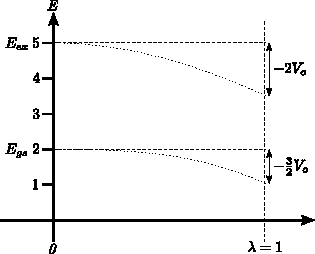
\includegraphics[width=0.6\textwidth]{Egs.pdf}
\end{figure}
\begin{align*}
	\tilde{E}^{(1)}_{ex}&= \int_{0}^{L}\int_{0}^{L}\frac{2}{L^2}\Bigg(\sin{\left(\frac{2\pi x_1}{L}\right)}
	\sin{\left(\frac{\pi x_2}{L}\right)}+\sin{\left(\frac{2\pi x_2}{L}\right)}\sin{\left(
	\frac{\pi x_1}{L}\right)}\Bigg)^2 \Bigg(-LV_o\mathlarger{\delta}(x_1,x_2)\Bigg)dx_1 dx_2\\
	&= \frac{L}{L^{2}}V_o 2\int_{0}^{L}\Bigg(2\sin{\left(\frac{2\pi x_1}{L}\right)}\sin{\left(
	\frac{\pi x_1}{L}\right)}\Bigg)^2 dx_1\\
	&= \frac{-8V_o}{L}\int_{0}^{L}\sin^2{\left(\frac{2\pi x_1}{L}\right)}\sin^2{\bigg(
	\frac{\pi x_1}{L}\bigg)}dx_1
\end{align*}
We solved this integral using a trigonometrical identity:
\begin{align*}
	Sin^2{(A)}Sin^2{(B)} &= Sin^2{(A)}-Sin^2{(A)}Cos^2{(B)}\\
	&=Sin^2(A)-\Bigg(\frac{Sin(A+B)-Sin(A-B)}{2}\Bigg)^2\\
	&= Sin^2 (A) - \frac{1}{4}\Bigg(Sin^2(A+B)-2Sin(A+B)Sin(A-B)+Sin^2(A-B)\Bigg)
\end{align*}
then, 
\begin{align*}
	& = \frac{-8V_o}{L}\int_{0}^{L}\cancelto{\frac{L}{2}}{Sin^2\left(\frac{2\pi x_1}{L}\right)}-
	\frac{1}{4}\Bigg(\cancelto{\frac{L}{2}}{Sin^2\left(\frac{3\pi x_1}{L}\right)}
	+\cancelto{\frac{L}{2}}{Sin^2\bigg(\frac{\pi x_1}{L}\bigg)}
	-\cancelto{\mathlarger{\delta_{mn}=0}}{2 Sin^2\left(\frac{3\pi x_1}{L}\right)
Sin\bigg(\frac{\pi x_1}{L}\bigg)}\Bigg)dx_1\\
	&= \frac{-8V_o}{L}\left(\frac{L}{2}-\frac{L}{4}\right)
\end{align*}
\begin{equation*}
	\boxed{\tilde{E}^{(1)}_{ex}= -2V_o}
\end{equation*}
\newpage
%%%%%%%%%%%%%%%%%%%%%%%%%%%%%%%%%%%%%%%%%%%%%%%%%%%%%%%%%%%%%%%%%%%%%%%%%%%%%%%%%%%%%%%%%%%%%%%%%%
%%%%%%%%%%%%%%%%%%%%%%%%%%%%%%%%%%%%%%%%%%%%%%%%%%%%%%%%%%%%%%%%%%%%%%%%%%%%%%%%%%%%%%%%%%%%%%%%%%
%%%%%%%%%%%%%%%%%%%%%%%%%%%%%%%%%%%%%%%%%%%%%%%%%%%%%%%%%%%%%%%%%%%%%%%%%%%%%%%%%%%%%%%%%%%%%%%%%
\chapter{Time Independent Degenerate Perturbation Theory}

\section{Lecture 7}
May 09, 2023\\
\\
1D infinite square well with two bosons
\begin{equation*}
	\mathlarger{\Psi}_{n_1 n_2}(x_1, x_2) = \frac{2}{L}\frac{1}{\sqrt{2}
		\sqrt{1+\mathlarger{\delta
	}_{n_1 n_2}}}\bigg(\sin{\left(\frac{n_1\pi x_1}{L}\right)}
	\sin{\left(\frac{n_2\pi x_2}{L}\right)}+\sin{\left(\frac{n_1\pi x_2}{L}\right)}
	\sin{\left(\frac{n_2\pi x_1}{L}\right)}\bigg)
\end{equation*}
Now, let's compute $\tilde{E}_{11}^{(2)}$
\begin{align*}
	\tilde{E}_{11}^{(2)} &= \left(1 - \mathlarger{\delta}_{n_1 n_2}\mathlarger{\delta}
		_{n_1 1}\right) \sum_{n_1,n_2=1}^{\infty}\frac{\big|\big<\mathlarger{\Psi}_{n_1 n_2}\big|-LV_o
	\mathlarger{\delta}(x_1-x_2)\big|\mathlarger{\Psi}_{11}\big>\big|^2}{E_{11}-E_{n_1 n_2}}\\
	&= \frac{2mL^2}{\pi^2 \hbar} \sum_{n_1,n_2}\frac{L^2V_o^2\left(1-\mathlarger{\delta}_{n_1 n_2}
	\mathlarger{\delta}_{n_1 1}\right)}{2-n_1^2 -n_2^2}\left(\frac{4}{L^2}\right)\frac{1}{2\left(
	1 +\mathlarger{\delta}_{n_1 n_2}\right)}\\
	&\cdot \bigg|\int_{0}^{L}\int_{0}^{L}\bigg[Sin\left(\frac{n_1 \pi x_1}{L}\right)Sin\left(\frac{n_2
	\pi x_2}{L}\right)+Sin\left(\frac{n_1 \pi x_2}{L}\right)\\
	& \cdot Sin\left(\frac{n_2 \pi x_1}{L}\right)\bigg]\mathlarger{\delta}(x_1-x_2)\bigg|^2
	\underbrace{\frac{2}{L}Sin\left(\frac{\pi x_1}{L}\right)Sin\left(\frac{\pi x_2}{L}
	\right)}_{\mathlarger{\Psi}_{11}(x_1, x_2)}dx_1 dx_2\\
	&= \frac{16mV_o^2}{\pi^2 \hbar^2}\sum_{n_1,n_2=1}^{\infty}\frac{1-\mathlarger{\delta}_{n_1n_2}
	\mathlarger{\delta}_{n_1 1}}{2-n_1^2-n_2^2}\frac{1}{1+\mathlarger{\delta}_{n_1 n_2}}
	\bigg|\int_{0}^{L}2 Sin\left(\frac{n_1 \pi x}{L}\right)
	Sin\left(\frac{n_2 \pi x}{L}\right)\underbrace{Sin^2\left(\frac{\pi x}{L}\right)}
	_{1-Cos^2\left(\frac{\pi x}{L}\right)}dx\bigg|^2\\
	&= \frac{2^6 m V_o^2}{\pi^2 \hbar^2} \sum_{n_1,n_2 =1}\frac{1-\mathlarger{\delta}_{n_1 n_2}
	\mathlarger{\delta}_{n_1 1}}{1+\mathlarger{\delta}_{n_1 n_2}}\frac{1}{2-n_1^2-n_2^2}
	\bigg|\underbrace{\int_{0}^{L} Sin\left(\frac{n_1 \pi x}{L}\right) Sin\left(\frac{n_2 \pi x}{L}\right)
	Sin^2\left(\frac{\pi x}{L}\right)dx}_{(*)}\bigg|^2
\end{align*}
Let's solve the integral $(*)$:
\begin{align*}
\int_{0}^{L} Sin\left(\frac{n_1 \pi x}{L}\right)
	Sin\left(\frac{n_2 \pi x}{L}\right)\underbrace{Sin^2\left(\frac{\pi x}{L}\right)}
	_{1-Cos^2\left(\frac{\pi x}{L}\right)}dx &= \cancelto{\frac{L}{2}\delta_{n_1n_2}}{\int_{0}^{L}
	Sin\left(\frac{n_1 \pi x}{L}\right)Sin\left(\frac{n_2 \pi x}{L}\right)dx}\\
	& -\int_{0}^{L}Sin\left(\frac{n_1 \pi x}{L}\right) Cos\left(\frac{\pi x}{L}\right)
	Sin\left(\frac{n_2 \pi x}{L}\right) Cos\left(\frac{\pi x}{L}\right)dx\\
	&= \frac{L}{2}\mathlarger{\delta}_{n_1n_2} -\frac{1}{4}\int_{0}^{L}Sin\left(\frac{(n_1+1)\pi x}
	{L}\right)Sin\left(\frac{(n_2+1)\pi x}{L}\right)\\
	& +Sin\left(\frac{(n_1+1)\pi x}{L}\right)Sin\left(\frac{(n_2-1)\pi x}{L}\right)\\
	&+ Sin\left(\frac{(n_1 -1)\pi x}{L}\right)Sin\left(\frac{(n_2+1)\pi x}{L}\right)\\
	&+ Sin\left(\frac{(n_1-1)\pi x}{L}\right)Sin\left(\frac{(n_2-1)\pi x}{L}\right)dx\\
	&= \frac{L}{2}\mathlarger{\delta}_{n_1n_2}-\frac{1}{4}\frac{L}{2}\left(\underbrace{\mathlarger
	{\delta}_{n_1+1,n_2+1}}_{\delta_{n_1n_2}} + \mathlarger{\delta}_{n_1+1,n_2-1}\right.\\
  & \left.+\mathlarger{\delta}
_{n_1-1,n_2+1}+\underbrace{\mathlarger{\delta}_{n_1-1,n_2-1}}_{\delta_{n_1n_2}}\right)\\
\end{align*}
Finally,
\begin{equation*}
	\tilde{E}_{11}^{(2)}=\frac{2^4 mL^2 V_o^2}{\pi^2 \hbar^2} \sum_{n_1,n_2 =1}\frac{1-\mathlarger{\delta}_{n_1 n_2}
	\mathlarger{\delta}_{n_1 1}}{1+\mathlarger{\delta}_{n_1 n_2}}\frac{1}{2-n_1^2-n_2^2}\bigg|
	\frac{\mathlarger{\delta}_{n_1n_2}}{2}-\frac{\mathlarger{\delta}_{n_1+1,n_2-1}+\mathlarger{\delta}
	_{n_1-1,n_2+1}}{4}\bigg|^2
\end{equation*}
we can notice that $n_1-n_2 = \pm 2\Rightarrow \Delta n = \pm 2$

\subsection*{Selection Rule}
$\Delta n = \mathcal{O}n \pm 2$
\begin{equation*}
		\tilde{E}_{11}^{(2)}=\frac{2V_o^2}{E_1} \sum_{n_1,n_2 =1}\frac{1-\mathlarger{\delta}_{n_1 n_2}
	\mathlarger{\delta}_{n_1 1}}{1+\mathlarger{\delta}_{n_1 n_2}}\frac{1}{2-n_1^2-n_2^2}\bigg|
	\underbrace{\mathlarger{\delta}_{n_1n_2}}_{\Delta n = 0}-
	\underbrace{\frac{\mathlarger{\delta}_{n_1+1,n_2-1}}{4}}_{\Delta n = -2}+
	\underbrace{\frac{\mathlarger{\delta}_{n_1-1,n_2+1}}{4}}_{\Delta n = +2}\bigg|^2
\end{equation*}
So, the ground state of two bosons only couples two exited states with the same or a difference
0f $\pm 2$ between the n's.
\subsection*{Time-Ind. Degenerate Perturbation Theory}
Suppose states $\mathbf{n, n+1, \cdots, n+k-1}$ are $k$-fold degenerate i.e. $\mathbf{
\mathcal{E}_n= \mathcal{E}_{n+1} = \cdots = \mathcal{E}_{n+k-1}}$, where $\mathbf{k}$ 
is the number of states with the same eigenenergy as $\mathbf{\mathcal{E}_n}$ for the 
unperturbed hamiltonian $\mathbf{\hat{H}_o}$.
\begin{align*}
	\hat{H}_o \big|\mathlarger{\psi}_n\big> &= \mathcal{E}_n\big|\mathlarger{\psi}_n \big>\\
	\big<\mathlarger{\psi}_n'\big|\mathlarger{\psi}_n\big> &= \mathlarger{\delta}_{n'n}\quad 
	\text{(Orthonormality)}
\end{align*}
Apply the perturbation $\hat{V}'$.\\
\\
The perturbed hamiltonian is $\tilde{H}=\hat{H}_o + \lambda V$, where $\lambda \in [0,1]$ is a 
bookkeeping parameter, and we expand the eigenenergies and eigenfunctions of the perturbed hamiltonian
in powers of $\lambda$.
\begin{equation*}
	\tilde{\mathcal{E}}_n = \tilde{\mathcal{E}}_n^{(0)}+\lambda \tilde{\mathcal{E}}_n^{(1)}
	+ \lambda^2 \tilde{\mathcal{E}}_n^{(2)} + \cdots = \sum_{k=0}\lambda^k 
	\tilde{\mathcal{E}}_n^{(k)}
\end{equation*}
so, $\lambda$ keeps track of the dependence on the perturbation $\hat{V}'$.
\begin{equation*}
	\therefore \tilde{\psi}_n = \tilde{\psi}_n^{(0)}+\lambda\tilde{\psi}_n^{(1)}+\lambda^2 
	+\lambda^2\tilde{\psi}_n^{(2)}+\cdots = \sum_{k=0}^{\infty}\lambda^k \tilde{\psi}_n^{(k)}
\end{equation*}
\subsection*{TISE}
\begin{equation*}
	\tilde{H}\big|\tilde{\psi}_n\big> = \tilde{\mathcal{E}}\big|\hat{\psi}_n\big>
\end{equation*}
Substituting for $\hat{H}, \big|\hat{\psi}_n\big>$ and $\tilde{\mathcal{E}}_n$:
\begin{equation*}
\left(\hat{H}_o + \lambda\hat{V}'\right) \sum_{k=0}^{\infty}\lambda^k \big|
\tilde{\psi}_n^{(k)}\big> = \sum_{k=0}^{\infty}\lambda^{k'}\tilde{\mathcal{E}}_n^{(k')}
\sum_{k=0}^{\infty}\lambda^{k}\big|\tilde{\psi}_n^{(k)}\big>
\end{equation*}
\[
\sum_{k=0}^{\infty}\left[\lambda^{k'}\hat{H}_o \big|\tilde{\psi}_n^{(k)}\big>
+ \lambda^{k+1}\hat{V}'\big|\tilde{\psi}_n^{(k)}\big> - \sum_{k'=0}^{k}\lambda^{k+k'}
\tilde{\mathcal{E}}_n^{(k')} \big|\tilde{\psi}_n^{(k)}\big>\right]=0\]
Gather together like powers of $\lambda$;
\[
	\sum_{k=0}^{\infty}\lambda^k\left[\hat{H}_o\big|\tilde{\psi}_n^{(k)}\big>+\hat{V}_o (
	1-\mathlarger{\delta}_{k0})\big|\tilde{\psi}_n^{(k-1)}\big>-\sum_{k'=0}^{k}
\tilde{\mathcal{E}}_n^{(k')}\big|\tilde{\psi}_n^{(k-k')}\big>\right] =0
\]
for this sum to be zero $\forall$ values of $\lambda$ we need the term in $[\cdots]$  to be zero
$\forall$ values of $k$ $\forall$ powers of $\lambda$.\\
\\
$\mathcal{O}(\lambda^0)=\mathcal{O}(1)=k=0$:
\[\hat{H}_o\big|\tilde{\psi}_n^{(0)} \big> = \tilde{\mathcal{E}}_n^{(0)}\big|\tilde{\psi}_n^{(0)}
\big>\quad {(\text{alternatively set }\lambda=0}\,\text{in TISE} )\]
multiply by $\big<\psi_{n'}\big|$: 
\[\big<\psi_{n'}\big|\hat{H}_o\big|\psi_{n}^{(0)}\big> = \tilde{\mathcal{E}}_n^{(0)} \big<\psi_{n'}
\big|\tilde{\psi}_n^{(0)}\big>\]
\begin{align*}
\big<\psi_{n'}\big|\hat{H}^\dagger_o\big|\psi_{n}^{(0)}\big>	-
\tilde{\mathcal{E}}_n^{(0)} \big<\psi_{n'}\big|\tilde{\psi}_n^{(0)}\big> &= 0\\
\mathcal{E}_{n'}\big<\psi_{n'}\big|\tilde{\psi}_n^{(0)}\big> -  
\tilde{\mathcal{E}}_n^{(0)} \big<\psi_{n'}\big|\tilde{\psi}_n^{(0)}\big> & = 0 \\
\left(\mathcal{E}_{n'}- \tilde{\mathcal{E}}_n^{(0)}\right)\tilde{\mathcal{E}}_n^{(0)} 
\big<\psi_{n'}\big|\tilde{\psi}_n^{(0)}\big> &= 0
\end{align*}
then, 
\[\Rightarrow \mathcal{E}_{n'} = \tilde{\mathcal{E}}_n^{(0)}\quad \text{or}\quad 
\big<\psi_{n'}\big|\tilde{\psi}_n^{(0)}\big> = 0\]
if $n' \in \{n, \cdots , n+k-1\}$, then $\mathcal{E}_{n'} = \mathcal{E}_n = \tilde{\mathcal{E}
}_n^{(0)}$
\begin{equation*}
	\Rightarrow \boxed{\big|\tilde{\psi}_n^{(0)}\big> = \sum_{n'=n}^{n+k-1}\big<\psi_{n'}\big|\tilde{
	\psi}_n^{(0)}\big>\big|\psi_{n'}\big>} 
\end{equation*}
So, the Zeroth order wave function for the $n^{th}$ perturbed eigenstate isn't just $\big|\psi_
{n'}\big>$, but a linear combination of all the \textbf{degenerate} unperturbed eigenfunctions 
with the same eigenvalue $\mathcal{E}_n$, i.e. 
\begin{align*}
	\big|\tilde{\psi}_n^{(0)}\big> &= \sum_{n'=n}^{n+k-1}
	\big<\psi_{n'}\big|\tilde{\psi}_n^{(0)}\big>\big|\psi_{n'}\big>\\
	&= \sum_{n'=n}^{n+k-1} C_{nn'}\big|\psi_{n'}\big> 
\end{align*}	
\begin{itemize}
	\item Sum over all degenerate unperturbed eigenstates. 
	\end{itemize}
and, 
\[\sum_{n'=n}^{n+k-1}\big|C_{n'n}\big|^2 = 1\]
\textbf{Idea:} the perturbation $\hat{V}'$ "lifts" the degeneracy between the k-fold degenerate
eigenstates of the unperturbed hamiltonian.\\
\\
The zeroth order eigenstate for the perturbed hamiltonian need to be eigenstates of the
perturbation. If the eigenstates of the unperturbed hamiltonian are also eigenstates of the 
perturbation, then we can just directly apply non-degenerate perturbation theory. 
\[\text{Recall:}\quad \tilde{\mathcal{E}}_n^{(1)} = \big<\psi_n \big|\hat{V}\big|\tilde{\psi}
_n^{(0)}\big>\]
So, we need to find $\big|\tilde{\psi}_n^{(0)}\big>$.
\newpage

%%%%%%%%%%%%%%%%%%%%%%%%%%%%%%%%%%%%%%%%%%%%%%%%%%%%%%%%%%%%%%%%%%%%%%%%%%%%%%%%%%%%%%%%%%%%%%%%%
%%%%%%%%%%%%%%%%%%%%%%%%%%%%%%%%%%%%%%%%%%%%%%%%%%%%%%%%%%%%%%%%%%%%%%%%%%%%%%%%%%%%%%%%%%%%%%%%%
%%%%%%%%%%%%%%%%%%%%%%%%%%%%%%%%%%%%%%%%%%%%%%%%%%%%%%%%%%%%%%%%%%%%%%%%%%%%%%%%%%%%%%%%%%%%%%%%%
\section{Lecture 8}
May 10, 2023\\
\\
Zeroth order term in the perturbed $n^{th}$ wavefunction, 
$$
\tilde{\psi}_n^{(0)}=\sum_{n'=n}^{n+k-1}\big<\psi_{n^{\prime}} 
\big| \tilde{\psi}_n^{(0)}\big>\big|\psi_{n^{\prime}}\big>
$$
where $\hat{H}_0\big|\psi_{n^{\prime}}\big>=
\mathcal{E}_n\big|\psi_{n'}\big>$ $\forall n^{\prime} \in\left\{n_1 \ldots,
n+k,-1\right\}$
(k-fold degenerate)
\[\sum_{n'=n}^{n+k-1}\big|\big<\psi_{n'} \big| \tilde
{\psi}_n^{(0)}\big>\big|^2=1\]
\begin{equation}
	\mathcal{O}(\lambda): \hat{H}_o \big|\tilde{\psi}_n^{(1)}\big> + \hat{V}'\big|\tilde{
	\psi}_n^{(0)}\big> = \tilde{\mathcal{E}}_n^{(o)}\big|\tilde{\psi}_n^{(1)}\big>+
	\tilde{\mathcal{E}}_n^{(1)}\big|\tilde{\psi}_n^{(0)}\big>
\end{equation}
We need to find $ \big|\tilde{\psi}_n^{(1)}\big>$ and $\tilde{\mathcal{E}}_n^{(1)}$,\\
\\
Multiply (3.2.1) by $\big<\psi_{n'}\big|$:
\[
	\big<\psi_{n'}\big|\hat{H}_o \big|\tilde{\psi}_n^{(1)}\big> + \big<\psi_{n'}\big|\hat{V}'
	\big|\tilde{\psi}_n^{(0)}\big> = \tilde{\mathcal{E}}_n^{(o)}\big<\psi_{n'}\big|\tilde{\psi}
	_n^{(1)}\big>+\tilde{\mathcal{E}}_n^{(1)}\big<\psi_{n'}\big|\tilde{\psi}_n^{(0)}\big>
\]
\[
	\left(\mathcal{E}_{n'}- \mathcal{E}_n\right)\big<\psi_{n'}\big|\tilde{\psi}_n^{(1)}\big> + \big<\psi_{n'}\big|\hat{V}'
	\big|\tilde{\psi}_n^{(0)}\big> =\tilde{\mathcal{E}}_n^{(1)}\big<\psi_{n'}\big|\tilde{\psi}_n^{(0)}\big>
\]\\
if $n' \in \{n, \cdots, n+k-1 \quad \text{and}\quad \mathcal{E}_{n'}=\mathcal{E}_n\}$, then:
\begin{align*}
  \tilde{\mathcal{E}_n^{(1)}} &= \frac{\big<\psi_{n'}\big|\hat{V}'\big|\psi_n^{(0)}\big>}
  {\big<\psi_{n'}\big|\tilde{\psi}_n^{(0)}\big>} = \frac{\big<\psi_{n'}\big|\hat{V}'\sum_{n''=n}
  ^{n+k-1} \big<\psi_{n''}\big|\tilde{\psi}_n^{(0)}\big>\big|\psi_{n''}   \big>}
  {\big<\psi_{n'}\big|\sum_{n''=n}^{n+k-1}\big<\psi_{n''}\big|\tilde{\psi}_n^{(0)}\big>\big| 
  \psi_{n''} \big>}\\
  &= \frac{\sum_{n''=n}^{n+k-1} C_{n'' n}\big<\psi_{n'}\big|\hat{V}\big|\psi_{n''}\big>}
  {\sum_{n''=n}^{n+k-1} C_{n''n}\big<\psi_{n'}\big|\psi_{n''}\big>}\\
  &= \frac{\sum_{n''=n}^{n+k-1} C_{n''n}\big<\psi_{n'}\big|\hat{V}\big| \psi_{n''} \big>}
  {C_{n'n}}
\end{align*}
\[
  \boxed{\tilde{\mathcal{E}}_n^{(1)} = \sum_{n''=n}^{n+k-1} \frac{C_{n''n}}{C_{n'n}} 
  \big<\psi_{n'}\big|\hat{V}\big|\psi_{n''} \big>}, \quad n' \in \{n, \cdots, n+k-1\}
\]\\
\\
This is a set of \emph{k} independet equations for $\tilde{\mathcal{E}}_n^{(1)}$, with 
different $C_{n'n}$:
\begin{itemize}
  \item $1+k$ equations
  \item $1 +k$ unknowns 
\end{itemize}
$\Rightarrow$ Closed system
\\
\\
\textbf{Matrix elements:} $W_{n'n''} = \big<\psi_{n'}\big|\hat{V}'\big|\psi_{n''} \big>$
\\
Expectation value of the perturbation $\big|\psi_{n''}\big>\longrightarrow \big<\psi_{n'}\big|$
\[
  \tilde{\mathcal{E}}_n^{(1)} = \sum_{n''=n}^{n+k-1} \frac{C_{n''n}}{C_{n'n}}W_{n'n''}
\]\\
\\
Consider \emph{k=2}, doubly degenerate system, 
$$\{n, n+1\} \equiv \{\alpha, \beta\}$$
\begin{equation*}
  \tilde{\mathcal{E}_n^{(1)}} = \frac{C_{\alpha \alpha}}{C_{\alpha \alpha}} W_{\alpha \alpha} +
  \frac{C_{\beta \alpha}W_{\alpha \beta}}{C_{\alpha \alpha}}, \quad n' = \alpha
\end{equation*}
\begin{equation*}
  \tilde{\mathcal{E}}_n^{(1)} = \frac{C_{\alpha \alpha}}{C_{\beta \alpha}} W_{\beta \alpha} + 
  \frac{C_{\beta \alpha} W_{\beta \beta}}{C_{\beta \alpha}},\quad  n' = \beta
\end{equation*}
Suppose $W_{\alpha\alpha} = W_{\beta\beta} = 0 \Rightarrow$ Perturbation between swaps eigenstates
of $\hat{H}_o$
\begin{equation*}
  \Rightarrow \tilde{\mathcal{E}}_{\alpha}^{(1)} = \frac{C_{\beta\alpha}}{C_{\alpha\alpha}}
  W_{\alpha\beta} = \frac{C_{\alpha\alpha}}{C_{\beta\alpha}}W_{\beta\alpha}
\end{equation*}
\[
  \big|C_{\alpha\alpha}\big|^2+ \big|C_{\beta\alpha}\big|^2 = 1
\]
\begin{equation*}
  \tilde{\mathcal{E}}_\alpha^{(1)} = \frac{\big|C_{\beta\alpha}\big|^2}{C_{\alpha\alpha}C_
  {\beta\alpha}} W_{\alpha\beta} = \frac{\big|C_{\alpha\alpha}\big|^2}{C_{\alpha\alpha}
C_{\beta\alpha}}W_{\beta\alpha}
\end{equation*}
\[
  C_{\alpha\alpha} = \frac{C_{\beta\alpha}W_{\alpha\beta}}{\tilde{\mathcal{E}}_\alpha^{(1)}}
\]
\[
  \tilde{\mathcal{E}}_\alpha^{(1)} = \cancelto{1}{\frac{C_{\beta\alpha}}{C_{\beta\alpha}}} 
  \frac{W_{\beta\alpha}W_{\alpha\beta}}{\tilde{\mathcal{E}_\alpha^{(1)}}}
\]
\[
  \big|\tilde{\mathcal{E}}_\alpha^{(1)}\big|^2 = \big|W_{\alpha\beta}\big|^2
\]
\begin{equation*}
  \boxed{\tilde{\mathcal{E}}_\alpha^{(1)} = \pm \big|\big<\psi_\alpha\big|\hat{V}\big|\psi_\beta
  \big>\big|}
\end{equation*}
\begin{enumerate}
  \item $C_{\alpha\alpha}\tilde{\mathcal{E}}_\alpha^{(1)} = C_{\alpha\alpha}W_{\alpha\alpha}+
    C_{\beta\alpha}W_{\alpha\beta}$\\
    \\
    Solve for $C_{\beta\alpha}:$
    \[
      C_{\beta\alpha} = C_{\alpha\alpha}\frac{\big(\tilde{\mathcal{E}_\alpha^{(1)}}-
      W_{\alpha\alpha}\big)}{W_{\alpha\beta}}
    \]
  \item $C_{\beta\alpha}\tilde{\mathcal{E}_\alpha^{(1)}} =C_{\alpha\alpha}W_{\beta\alpha}+ 
    C_{\beta\alpha}W_{\beta\beta}$\\
    \\
    Substituting in for $C_{\beta\alpha}:$
    \[
      C_{\alpha\alpha} \frac{\big(\tilde{\mathcal{E}_\alpha^{(1)}}- W_{\alpha\alpha}\big)}
      {W_{\alpha\beta}}\tilde{\mathcal{E}_\alpha^{(1)}} = C_{\alpha\alpha}W_{\beta\alpha}
      + C_{\alpha\alpha}\frac{\big(\tilde{\mathcal{E}_\alpha^{(1)}}- W_{\alpha\alpha}\big)}
      {W_{\alpha\beta}}W_{\beta\beta}
    \]
\end{enumerate}
Factor out $C_{\alpha\alpha}$ and multiply by $W_{\alpha\beta}$, and rearrange in powers of 
$\tilde{\mathcal{E}}_\alpha^{(1)}$:
\[
  C_{\alpha\alpha}\left[\left(\tilde{\mathcal{E}}_\alpha^{(1)}\right)^2-\left( 
  W_{\alpha\alpha}+W_{\beta\beta}\right)\tilde{\mathcal{E}}_\alpha^{(1)}  - \big|W_{\alpha
\beta}\big|^2+W_{\alpha\alpha}W_{\beta\beta}\right] = 0
\]
\[
  \therefore C_{\beta\alpha}\left[\left(\tilde{\mathcal{E}}_\alpha^{(1)}\right)^2 - 
  \left(W_{\alpha\alpha}+W_{\beta\beta}\right)\tilde{\mathcal{E}}_\alpha^{(1)} - 
\big|W_{\alpha\beta}\big|^2 + W_{\alpha\alpha}W_{\beta\beta}\right]=0
\]\\
So, either $C_{\alpha\alpha} = 0, C_{\beta\alpha} = 0,$ or $\left(\tilde{\mathcal{E}}_\alpha^{(1)}
\right) - \left(W_{\alpha\alpha}+W_{\beta\beta}\right)\tilde{\mathcal{E}}_\alpha^{(1)}
- \big|W_{\alpha\beta}\big|^2 + W_{\alpha\alpha}W_{\beta\beta} = 0$\\
\\
If $C_{\alpha\alpha} = 0 \Rightarrow \big|\tilde{\psi}_\alpha^{(0)}\big> = \big|\psi_\beta\big>$, 
if $C_{\beta\alpha} = 0 \Rightarrow \big|\tilde{\psi}_\alpha^{(0)}\big> = \big|\tilde{\psi}_
\alpha\big>$\\
\\
Since $\big|C_{\alpha\alpha}\big|^2 + \big|C_{\beta\alpha}\big|^2 = 1$, and we can just use 
T.I.N.D.P.T\\
\\
Otherwise
\[ 
  \tilde{\mathcal{E}}_\alpha^{(1)} = \frac{W_{\alpha\alpha}+W_{\beta\beta}}{2} \pm 
  \sqrt{\frac{\left(W_{\alpha\alpha}+W_{\beta\beta}\right)^2}{4}+ \big|W_{\alpha\beta}\big|^2 
  - W_{\alpha\alpha}W_{\beta\beta}}
\]
Then we've got two solutions $\pm W$\\
\\
Figure\\
\\
\[
  \tilde{\mathcal{E}}_\alpha^{(1)} = \underbrace{{\frac{W_{\alpha\alpha}+W_{\beta\beta}}{2}}
  }_{\text{$(*)$}} \pm \sqrt{\frac{W_{\alpha\alpha}^2 + 2W_{\alpha\alpha}W_{\beta\beta}+W_{\beta
  \beta}^2}{4} - W_{\alpha\alpha}W_{\beta\beta}+\big|W_{\alpha\beta}\big|^2}
\]
here $(*)$ is the average of \emph{T.I.N.D.P.T} results for $\tilde{\mathcal{E}}_\alpha$ and 
$\tilde{\mathcal{E}}_\beta$.
\[
  =\frac{W_{\alpha\alpha}W_{\beta\beta}}{2} \pm \sqrt{\left(\frac{W_{\alpha\alpha}
  - W_{\beta\beta}}{2}\right)^2 + \big|W_{\alpha\beta}\big|^2}
\]
\begin{itemize}
  \item $\frac{W_{\alpha\alpha}
  - W_{\beta\beta}}{2} $ is half the absolute difference between $W_{\alpha\alpha}$ and 
    $W_{\beta\beta}$
\end{itemize}
two eigenvalues of the matrix:\\ 
\[
\det\begin{vmatrix}
  \lambda-W_{\alpha\alpha} & W_{\alpha\beta} \\
  W_{\beta\alpha} & \lambda-W_{\beta\beta}
\end{vmatrix} = 0
\]
\\
If $W_{\alpha\beta}=0$ (i.e. $\big|\psi_\alpha\big>$ and $\big|\psi_\beta\big>$ are eigenstates of the 
perturbation $\hat{V}'$) then: 
\begin{align*}
  \tilde{\mathcal{E}}_\alpha^{(1)} &= \frac{W_{\alpha\alpha}+W_{\beta\beta}}{2} \pm
  \frac{\big|W_{\alpha\alpha}-W_{\beta\beta}\big|}{2}= \text{max/min}\left(W_{\alpha\alpha},W
  _{\beta\beta}\right)\\
  \tilde{\mathcal{E}}_\alpha^{(1)}&= \text{min}\left(W_{\alpha\alpha},W_{\beta\beta}\right)\\
\tilde{\mathcal{E}}_\beta^{(1)}&= \text{max}\left(W_{\alpha\alpha},W_{\beta\beta}\right)
\end{align*}
\[
  \mathcal{W}_{n'n}= \big<\psi_n\big|\hat{V}\big|\psi_{n'}\big>\Rightarrow \mathcal{W} = 
  \begin{pmatrix} 
    \big<\psi_n\big|\hat{V}\big|\psi_n\big> & \dots  &  \big<\psi_n\big|\hat{V}\big|\psi_
    {n+k-1}\big>\\
    \vdots & \ddots & \vdots\\
    \big<\psi_{n+k-1}\big|\hat{V}\big|\psi_n\big> & \dots  &  
    \big<\psi_{n+k-1}\big|\hat{V}\big|\psi_{n+k-1}\big> 
    \end{pmatrix}
\]
Solve the eigen problem:\\
\[
  \det[\lambda I - \mathcal{W}] = 0
\]\\
What are $\big|\tilde{\psi}_\alpha^{(0)}\big>$ and $\big|\tilde{\psi}_\beta^{(0)}\big>$? i.e. 
$\big|\psi_\pm\big> = C_{\alpha\pm}\big|\psi_\alpha\big> + C_{\beta\pm}\big|\psi_\beta\big>$
\[
  C_{\alpha\pm}W_{\alpha\alpha} + C_{\beta\pm}W_{\alpha\beta} = \tilde{\mathcal{E}}_\pm^{(1)}
  C_{\alpha\pm}
\]
\[
  C_{\alpha\pm}W_{\beta\alpha}+C_{\beta\pm}W_{\beta\beta} = \tilde{\mathcal{E}}_\pm^{(1)} 
  C_{\beta\pm}
\]
\[\big|C_{\alpha\pm}\big|^2 + \big|C_{\beta\pm}\big|^2 = 1\]\\
\begin{empheq}[box=\fbox]{align*}
  C_{\alpha\pm} &= \frac{C_{\beta\pm}W_{\alpha\beta}}{\tilde{\mathcal{E}}_\pm^{(1)}-W_{\alpha\alpha}} \\
  C_{\beta\pm}&= C_{\alpha\pm}\frac{\left(\tilde{\mathcal{E}}_\pm^{(1)}-W_{\alpha\alpha}\right)}
  {W_{\alpha\beta}}
\end{empheq}
\\
\begin{align*}
  \big<\psi_\mp\big|\psi_\pm \big> &= \left(C_{\alpha\mp} \big<\psi_\alpha\big| + C_{\beta\mp}
  \big<\psi_\beta\big| \right)\left(C_{\alpha\pm}\big|\psi_{\alpha}\big> + C_{\beta\pm} 
  \big|\psi_\beta\big>\right)\\
  &= C_{\alpha\mp}C_{\alpha\pm}\big<\psi_\alpha\big|\psi_\alpha\big> + C_{\alpha\mp}C_{\beta\pm}
  \big<\psi_\alpha\big|\psi_\beta\big>+C_{\beta\mp}C_{\alpha\pm}\big<\psi_\beta\big|
  \psi_\alpha\big>+C_{\beta\mp}C_{\beta\pm}\big<\psi_\beta\big|\psi_\beta\big>\\
  &=C_{\alpha\mp}C_{\alpha\pm}\cancelto{1}{\mathlarger{\delta}_{\alpha\alpha}}  +  
  C_{\alpha\mp}C_{\beta\pm}\cancelto{0}{\mathlarger{\delta}_{\alpha\beta}} +
  C_{\beta\mp}C_{\alpha\pm}\cancelto{0}{\mathlarger{\delta}_{\beta\alpha}} +
  C_{\beta\mp}C_{\beta\pm}\cancelto{1}{\mathlarger{\delta}_{\beta\beta}}\\
  &=C_{\alpha\mp}C_{\alpha\pm}+C_{\beta\mp}C_{\beta\pm} 
\end{align*}
\[
  \boxed{\tilde{\mathcal{E}}_\pm^{(1)}=\frac{W_{\alpha\alpha} +W_{\beta\beta}}{2} \pm 
  \sqrt{\left(\frac{W_{\alpha\alpha}
  - W_{\beta\beta}}{2}\right)^2 + \big|W_{\alpha\beta}\big|^2}}
\]
%%%%%%%%%%%%%%%%%%%%%%%%%%%%%%%%%%%%%%%%%%%%%%%%%%%%%%%%%%%%%%%%%%%%%%%%%%%%%%%%%%%%%%%%%%%%%%%%%
%%%%%%%%%%%%%%%%%%%%%%%%%%%%%%%%%%%%%%%%%%%%%%%%%%%%%%%%%%%%%%%%%%%%%%%%%%%%%%%%%%%%%%%%%%%%%%%%%
%%%%%%%%%%%%%%%%%%%%%%%%%%%%%%%%%%%%%%%%%%%%%%%%%%%%%%%%%%%%%%%%%%%%%%%%%%%%%%%%%%%%%%%%%%%%%%%%%
%%%%%%%%%%%%%%%%%%%%%%%%%%%%%%%%%%%%%%%%%%%%%%%%%%%%%%%%%%%%%%%%%%%%%%%%%%%%%%%%%%%%%%%%%%%%%%%%%
\newpage
\section{Lecture 9}
May 15, 2023\\
\\
Suppose we have two degenerate wavefunctions with energy $\mathcal{E}$ for the unperturbed 
hamiltonian, $\alpha, \beta$
\[
  \hat{H}_o\big|\psi_\alpha\big> = \mathcal{E}\big|\psi_\alpha\big>
\]
\[
  \hat{H}_o\big|\psi_\beta\big> = \mathcal{E}\big|\psi_\beta\big>
\]
We know that:
\begin{align*}
  &\big<\psi_i\big|\psi_j\big>= \mathlarger{\delta}_{ij}\\ 
  &\hat{H} = \hat{H_o} + \lambda \hat{V}'\\
  &\big|\tilde{\psi}_\pm\big>= C_{\alpha\pm}\big|\psi_\alpha\big> + C_{\beta\pm}\big|
  \psi_\beta\big>\\
  &\big|C_{\alpha\pm}\big|^2 + \big|C_{\beta\pm}\big|^2 = 1
\end{align*}
\begin{equation*}
  \tilde{\mathcal{E}}_\pm^{(1)} =\frac{ \big<\psi_\alpha\big|\hat{V}'\big|\psi_\alpha\big>+
  \big<\psi_\beta\big|\hat{V}'\big|\psi_\beta\big>}{2}+ 
  \sqrt{\left(\frac{\big<\psi_\alpha\big|\hat{V}'\big|\psi_\alpha\big>- 
  \big<\psi_\beta\big|\hat{V}'\big|\psi_\beta\big>}{2}\right)^2+
\big|\big<\psi_\alpha\big|\hat{V}'\big|\psi_\beta\big>\big|^2}
\end{equation*}
\begin{itemize}
  \item The first term is the average of \emph{T.I.N.D.P.T} $\mathcal{O}(\lambda)$ correction for 
$\tilde{\mathcal{E}}_\alpha^{(1)} $ and $ \tilde{\mathcal{E}}_\beta^{(1)} $.
\item The first term in the root is the difference between $\tilde{\mathcal{E}}_\alpha^{(1)}
  $ and $ \tilde{\mathcal{E}}_\beta^{(1)} $  and their average.
\item The last term in the root is the cross term non-zero when $\big|\psi_\alpha\big>$ and 
  $\big|\psi_\beta\big>$ are not eigenstates of $\hat{V}'$.
\end{itemize}
Let $\omega_\pm = \tilde{\mathcal{E}}_\pm^{(1)}$:
\begin{equation}
  \omega_\pm =\frac{W_{\alpha\alpha} +W_{\beta\beta}}{2} \pm 
  \sqrt{\left(\frac{W_{\alpha\alpha}
  - W_{\beta\beta}}{2}\right)^2 + \big|W_{\alpha\beta}\big|^2} 
\end{equation}
(\emph{TISE}) to $\mathcal{O}(\lambda)$ and multiply by $\big<\psi_\alpha\big|$:
\[
  \big<\psi_\alpha\big|\hat{V}'\left(C_{\alpha\pm}\big|\psi_{\alpha}\big> + C_{\beta\pm} 
  \big|\psi_\beta\big>\right) = \mathcal{E}_\pm C_{\alpha\pm}
\]
\begin{equation}
  C_{\alpha\pm} \left(\mathcal{E}_\pm - W_{\alpha\alpha}\right) = C_{\beta\pm}W_{\alpha\beta}
  \Rightarrow C_{\beta\pm}=C_{\alpha\pm}\frac{\left(\tilde{\mathcal{E}}_\pm - W_{\alpha\alpha}
  \right)}{W_{\alpha\beta}}
\end{equation}
$\therefore$ multiply by $\big<\psi_\beta\big|$:
\[
   \big<\psi_\beta\big|\hat{V}'\left(C_{\alpha\pm}\big|\psi_{\alpha}\big> + C_{\beta\pm} 
  \big|\psi_\beta\big>\right) = \mathcal{E}_\pm C_{\beta\pm}
\]
\[
  C_{\beta\pm} \left(\mathcal{E}_\pm - W_{\beta\beta}\right) = C_{\alpha\pm}W_{\beta\alpha}
\]
\[
  C_{\alpha\pm} \left[\left( \mathcal{E}_\pm - W_{\alpha\alpha}\right) 
  \left(\mathcal{E}_\pm - W_{\beta\beta}\right) - W_{\alpha\beta}W_{\beta\alpha}\right] = 0
\]
Are the eigenstates we got orthogonal?
\[
  \big<\psi_+\big|\psi_-\big> = \left(C_{\alpha +}^*\big<\psi_\alpha\big| + C_{\beta +}^* 
  \big<\psi_\beta\big|\right)\left(C_{\alpha_\mp}\big|\psi_\alpha \big> + C_{\beta -}
  \big|\psi_\beta\big>\right)
\]
\begin{align*}
  \big<\psi_i\big|\psi_j\big> &= \mathlarger{\delta}_{ij},\quad \text{Using orthonormality of the eigenstates}\\
&= C_{\alpha +}C_{\alpha -}+ C_{\beta +}C_{\beta -}, \quad \text{Substitute in (3.3.2) for}
\,C_{\beta\pm}\\
&= C^*_+ C_- \left[1 + \frac{\left(\mathcal{E}_+ - W_{\alpha\alpha}\right)}{W_{\alpha\beta}}
\frac{\left(\mathcal{E}_- - W_{\alpha\alpha}\right)}{W_{\alpha\beta}}\right]
\end{align*}
Substitute in (3.3.1) for $\mathcal{E}_\pm$:
\begin{align*}
  &=C^*_{\alpha +}C_{\alpha -} \Biggl[1+\frac{\left(\frac{W_{\alpha\alpha}+W_{\beta\beta}}{2} +
  \sqrt{\left(\frac{W_{\alpha\alpha}+W_{\beta\beta}}{2}\right)^2 + \big|W_{\alpha\beta}
\big|^2 }-W_{\alpha\alpha}\right)  }{\left(W_{\alpha\beta}\right)^2}\\
  &\cdot\left(\frac{W_{\alpha\alpha}+W_{\beta\beta}}{2} - W_{\alpha\alpha} - \sqrt{
\left(\frac{W_{\alpha\alpha}-W_{\beta\beta}}{2}\right)^2+\big|W_{\alpha\beta}\big|^2}\right)\Biggr]\\
&=C^*_{\alpha +}C_{\beta -}\Bigg[1+\frac{1}{\big|W_{\alpha\beta}\big|^2} 
\left(\frac{W_{\beta\beta}-W_{\alpha\alpha}}{2} +
\sqrt{\left(\frac{W_{\alpha\alpha}-W_{\beta\beta}}{2}\right)^2 + \big|W_{\alpha\beta}
\big|^2 }\right)\\
&\cdot\left(\frac{W_{\beta\beta}-W_{\alpha\alpha}}{2}-
\sqrt{\left(\frac{W_{\alpha\alpha}-W_{\beta\beta}}{2}\right)^2 + \big|W_{\alpha\beta}
\big|^2 }\right)\Bigg] 
\end{align*}
Since $(x+y)(x-y) = x^2-y^2$, cross terms cancel:
\begin{align*}
  &= C_{\alpha +}C_{\beta -} \left[ 1+\frac{1}{\big|W_{\alpha\beta}\big|^2}\left[
      \Bigg|\frac{W_{\beta\beta}-W_{\alpha\alpha}}{2}\Bigg|^2- \Bigg|\frac{
  W_{\alpha\alpha}-W_{\beta\beta}}{2}\Bigg|^2 + \big|W_{\alpha\beta}\big|^2\right]\right]\\
  &\boxed{= C_{\alpha +}C_{\alpha -}[1-1] = 0}
\end{align*}
\[
  \boxed{\big<\psi_\pm\big|\psi_\mp\big> = 0 }
\]
\begin{align*}
  &\big<\psi_\pm\big|\psi_\mp\big> = \left(C_{\alpha \pm}^*\big<\psi_\alpha\big| + C_{\beta \pm}^* 
  \big<\psi_\beta\big|\right)\left(C_{\alpha_\mp}\big|\psi_\alpha \big> + C_{\beta\mp}
  \big|\psi_\beta\big>\right)\\
  &\big<\psi_\pm\big|\psi_\mp\big> = C_{\alpha \pm}^* C_{\alpha\mp}\big<\psi_\alpha\big|\psi_
  \alpha\big>+C_{\alpha\pm}^*C_{\beta\mp}\big<\psi_\alpha\big|\psi_ \beta\big> + C_{\beta\pm}^*
  C_{\alpha\mp}\big<\psi_\beta\big|\psi_ \alpha\big>+C_{\beta\pm}^*C_{\beta\mp} 
  \big<\psi_\beta\big|\psi_ \beta\big>\\
  & \big<\psi_\pm\big|\psi_\mp\big>=  C_{\alpha \pm}^* C_{\alpha\mp} + C_{\beta\pm}^*C_{\beta\mp}=
   C_{\alpha \pm}^* C_{\alpha\mp} + C_{\alpha\pm}^*\left(\frac{\mathcal{E}_\pm - W_{\alpha\alpha}
   }{W_{\alpha\beta}}\right)^* C_{\alpha\mp}\left(\frac{\mathcal{E}_\mp - W_{\alpha\alpha}}
 {W_{\alpha\beta}}\right)\\
 &\big<\psi_\pm\big|\psi_\mp\big> = C_{\alpha \pm}^* C_{\alpha \mp}\Bigg[1+ \frac{1}{\big|W_{
     \alpha\beta}\big|^2}\left(\frac{W_{\beta\beta}-W_{\alpha\alpha}}{2}\pm 
     \sqrt{\left(\frac{W_{\alpha\alpha}-W_{\beta\beta}}{2}\right)^2+\big|W_{\alpha\beta}\big|}
   \right)^*\\
 &\cdot \left(\frac{W_{\beta\beta}-W_{\alpha\alpha}}{2} \mp \sqrt{\left(\frac{W_{\alpha\alpha}-
W_{\beta\beta}}{2}\right)^2 + \big|W_{\alpha\beta}\big|^2}\right)\Bigg]\\
  &\big<\psi_\pm\big|\psi_\mp\big> = C_{\alpha \pm}^* C_{\alpha \mp}\Bigg[1+ \frac{1}{\big|W_{
    \alpha\beta}\big|^2}\left( \Bigg|\frac{W_{\beta\beta}-W_{\alpha\alpha}}{2}\Bigg|^2- \Bigg|\frac{
  W_{\alpha\alpha}-W_{\beta\beta}}{2}\Bigg|^2 + \big|W_{\alpha\beta}\big|^2\right)\\
  &=C_{\alpha \pm}^* C_{\alpha \mp}(1-1) = 0
\end{align*}
\begin{align*}
  \big<\psi_\pm\big|\psi_\pm\big>& = \left(C_{\alpha \pm}^*\big<\psi_\alpha\big| + C_{\beta \pm}^* 
  \big<\psi_\beta\big|\right)\left(C_{\alpha_\pm}\big|\psi_\alpha \big> + C_{\beta\pm}
  \big|\psi_\beta\big>\right)\\
  &=C_{\alpha \pm}^* C_{\alpha\pm}\big<\psi_\alpha\big|\psi_
  \alpha\big>+C_{\alpha\pm}^*C_{\beta\pm}\big<\psi_\alpha\big|\psi_ \beta\big> + C_{\beta\pm}^*
  C_{\alpha\pm}\big<\psi_\beta\big|\psi_ \alpha\big>+C_{\beta\pm}^*C_{\beta\pm} 
  \big<\psi_\beta\big|\psi_ \beta\big>\\
  &= \big|C_{\alpha \pm}\big|^2 + \big|C_{\beta \pm} \big|^2 = 1\quad \text{by construction!}
\end{align*}
\begin{equation*}
  C_{\beta\pm}= C_{\alpha\pm}\frac{\left(\mathcal{E}_{\pm} - W_{\alpha\alpha}\right)}{W_{\alpha\beta}}
  =\frac{C_{\alpha\pm}}{W_{\alpha\beta}}\left(\frac{W_{\beta\beta}-W_{\alpha\alpha}}{2}\pm
  \sqrt{\left(\frac{W_{\alpha\alpha}-W_{\beta\beta}}{2}\right)^2 + \big|W_{\alpha\beta}\big|^2}\right)
\end{equation*}
\begin{align*}
  \big<\psi_\pm\big|\hat{V}\big|\psi_\mp\big>&= \left(C_{\alpha\pm}^*\big<\psi_\alpha\big|
  C_{\beta\pm}^*\big<\psi_\beta\big|\right)\hat{V}'\left(C_{\alpha\mp}\big|\psi_\alpha\big>
  + C_{\beta\mp}\big|\psi_{\beta\mp}\big>\right)\\
  &= C_{\alpha\pm}^*C_{\alpha\mp}\big<\psi_\alpha\big|\hat{V}'\big|\psi_{\alpha}\big> + 
  C_{\alpha\pm}^*C_{\beta\mp}\big<\psi_\alpha\big|\hat{V}'\big|\psi_{\beta}\big>+C_{\beta\pm}^*
  C_{\alpha\mp}\big<\psi_\beta\big|\hat{V}'\big|\psi_{\alpha}\big>+C_{\beta\pm}^*C_{\beta\mp}
  \big<\psi_\beta\big|\hat{V}'\big|\psi_{\beta}\big>\\
  &= C_{\alpha\pm}^*C_{\alpha\mp}W_{\alpha\alpha}+\frac{C_{\alpha\pm}^*C_{\alpha\mp}}
  {\cancel{W_{\alpha\beta}}}\left(\mathcal{E}_- - W_{\alpha\alpha}\right)\cancel{W_{\alpha\beta}}
  + C_{\alpha\pm}^*C_{\alpha\mp}\left(\frac{\mathcal{E}_+ - W_{\alpha\alpha}}{\cancel{
  W_{\alpha\beta}}}\right)^*\cancel{W_{\beta\alpha}} \\
  & + C_{\alpha\pm}^* C_{\alpha\mp}\left(\frac{\mathcal{E}_+ - W_{\alpha\alpha}}{W_{\alpha\beta}
  } \right)^*\left(\frac{\mathcal{E}_- - W_{\alpha\alpha}}{W_{\alpha\beta}}\right)W_{\beta\beta}\\
  &= C_{\alpha\pm}^*C_{\alpha\mp}\left[W_{\alpha\alpha}+\mathcal{E}_- -W_{\alpha\alpha} +
  \mathcal{E}_+ - W_{\alpha\alpha}+\frac{W_{\beta\beta}}{\big|W_{\alpha\beta}\big|^2} 
\left(\frac{W_{\beta\beta}- W_{\alpha\alpha}}{2}\right. \right.\\
  &\left.\left. +\sqrt{\left(\frac{W_{\alpha\alpha}-W_
{\beta\beta}}{2}\right)^2+\big|W_{\alpha\beta}\big|^2}\right)^*
\cdot\left(\frac{W_{\beta\beta}-W_{\alpha\alpha}}{2} - \sqrt{\left(\frac{W_{\alpha\alpha}-
W_{\beta\beta}}{2}\right)^2+\big|W_{\alpha\beta}\big|^2}\right)\right]
\end{align*}

\begin{align*}
  &= C_{\alpha\pm}^*C_{\alpha\mp}\left[W_{\alpha\alpha}+W_{\beta\beta}-W_{\alpha\alpha} + 
    \frac{W_{\beta\beta}}{\big|\cancel{W_{\alpha\beta\big|^2}}}\left(\cancel{\Bigg|\frac{W_{\beta\beta}-
  W_{\alpha\alpha}}{2}\Bigg|^2}\right. \right.\\
  &\left. \left. -\cancel{\Bigg|\frac{W_{\alpha\alpha}-
W_{\beta\beta}}{2}\Bigg|^2}-\cancel{\big|W_{\alpha\beta}\big|^2} \right)\right]\\
  &= \boxed{C_{\alpha\pm}^* C_{\alpha\mp}\left(W_{\alpha\alpha}+W_{\beta\beta}-W_{\alpha\alpha}-
  W_{\beta\beta}\right) = 0}
 \end{align*}
 $\Rightarrow$ $\big|\psi_\pm\big>$ are eigenstates of $\hat{V}'$\\
 \\
 \textbf{What are their eigenvalues?} i.e $\hat{V}'\big|\psi_\pm\big> = \mathcal{E}_\pm \big|
 \psi_\pm\big>$
 \begin{align*}
 \big<\psi_\pm\big|\hat{V}\big|\psi_\pm\big>&= \left(C_{\alpha\pm}^*\big<\psi_\alpha\big|
  C_{\beta\pm}^*\big<\psi_\beta\big|\right)\hat{V}'\left(C_{\alpha\pm}\big|\psi_\alpha\big>
  + C_{\beta\pm}\big|\psi_{\beta\mp}\big>\right)\\
    &= C_{\alpha\pm}^*C_{\alpha\pm}\big<\psi_\alpha\big|\hat{V}'\big|\psi_{\alpha}\big> + 
  C_{\alpha\pm}^*C_{\beta\pm}\big<\psi_\alpha\big|\hat{V}'\big|\psi_{\beta}\big>+C_{\beta\pm}^*
  C_{\alpha\pm}\big<\psi_\beta\big|\hat{V}'\big|\psi_{\alpha}\big>\\
    &+C_{\beta\pm}^*C_{\beta\pm}\big<\psi_\beta\big|\hat{V}'\big|\psi_{\beta}\big>\\
    &= \big|C_{\alpha\pm}\big|^2W_{\alpha\alpha}+C_{\alpha\pm}^*C_{\beta\pm}W_{\alpha\beta}+
    C_{\beta\pm}^*C_{\alpha\pm}W_{\beta\alpha}+\big|C_{\beta}\big|^2W_{\beta\beta}
\end{align*}
whe know that:
\[
  C_{\alpha\pm} = C_{\beta\pm}\left(\frac{\mathcal{E}_\pm - W_{\beta\beta}}{W_{\beta\alpha}}
    \right), \quad C_{\beta\pm} = C_{\alpha\pm}\left(\frac{\mathcal{E}_\pm - W_{\alpha\alpha}}{
        W_{\alpha\beta}
    }\right)
\]
then, 
\begin{align*}
  \big<\psi_\pm\big|\hat{V}\big|\psi_\pm\big>&=
  \big|C_{\alpha_\pm}\big|^2\left(\cancel{W_{\alpha\alpha}}+\frac{\mathcal{E}_\pm -
  \cancel{W_{\alpha\alpha}}}{\cancel{W_{\alpha\beta}}}\cdot \cancel{W_{\alpha\beta}}\right)
  +\big|C_{\beta_\pm}\big|^2\left(\cancel{W_{\beta\beta}}+\frac{\mathcal{E}_\pm -
  \cancel{W_{\beta\beta}}}{\cancel{W_{\beta\alpha}}}\cdot \cancel{W_{\beta\alpha}}\right)\\
  &\boxed{= \mathcal{E}_\pm \left(\big|C_{\alpha\pm}\big|^2+\big|C_{\beta\pm} \big|^2\right)
  = \mathcal{E}_\pm}
\end{align*}
So, $\big|\psi_\pm\big>$ are eigenstates of the perturbation $\hat{V}'$ and their eigenvalues
are $\mathcal{E}_\pm$, i.e, the first order correction in $\hat{V}'$ to the eigenenergies 
of the perturbed hamiltonian $\hat{H} = \hat{H}_o + \hat{V}'$.\\
\\
If $W_{\alpha\beta}=0=\big<\psi_\alpha\big|\hat{V}'\big|\psi_\beta\big>$, then $\big|\psi_\alpha
\big>$ and $\big|\psi_\beta\big>$ are eigenstates of $\hat{V}'$ and we can use non-degenerate
perturbation theory. 
\newpage
\subsection{Example: A 1D periodic space of length $L$, i.e, a Ring.}
\begin{wrapfigure}{l}{6cm}
  \begin{center}
    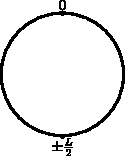
\includegraphics[width=0.2\textwidth]{1D_L.pdf}
  \end{center}
\end{wrapfigure}
\
\
Find the eigenstates of a particle to a 1D ring. 
\[\text{\emph{TISE}:}\quad \frac{-\hbar^2}{2m}\frac{d^2}{dx^2}\Psi(x) = \mathcal{E}\Psi(x)\]
(B.C): 
\begin{align*}
&\Psi(\pm L) = 0\\
&\Psi''(x)= \frac{-2m}{\hbar^2}\mathcal{E}\Psi(x)
\end{align*}
\[
  \Rightarrow \Psi \left(\frac{L}{2}\right) = Ae^{\left(i\sqrt{\frac{2m\mathcal{E}}{\hbar^2}}
    \frac{L}{2}\right)}+
  Be^{\left(-i\sqrt{\frac{2m\mathcal{E}}{\hbar^2}}\frac{L}{2}\right)}= \Psi\left(\frac{-L}{2}\right)
\]
\[= Ae^{\left(-i\sqrt{\frac{2m\mathcal{E}}{\hbar^2}}\frac{L}{2}\right)} + 
Be^{\left(i\sqrt{\frac{2m\mathcal{E}}{\hbar^2}}\frac{L}{2}\right)}\]\\
\[\left(A-B\right)e^{\left(i\sqrt{\frac{2m\mathcal{E}}{\hbar^2}}\frac{L}{2}\right)}=
\left(A-B\right)e^{\left(-i\sqrt{\frac{2m\mathcal{E}}{\hbar^2}}\frac{L}{2}\right)}\]
\begin{align*}
  \left(A-B\right)\left(e^{\left(i\sqrt{\frac{2m\mathcal{E}}{\hbar^2}}\frac{L}{2}\right)
  }-1\right) = 0
\end{align*}
\[
  \Rightarrow e^{\left(i\sqrt{\frac{2m\mathcal{E}}{\hbar^2}}\frac{L}{2}\right)} = 1 
  \longrightarrow e^{i2\pi n} = 0, \quad\forall n \in \mathbb{Z} 
\]
\[
  \Rightarrow \sqrt{\frac{2m\mathcal{E}}{\hbar^2}}L = 2\pi n,\quad n \in \mathbb{Z}
\]
Then, the eigenenergies are given by:
\[
  \mathcal{E}_n = \frac{4\hbar^2 \pi^2 n^2 }{2mL^2} = \frac{2\hbar^2 \pi^2 n^2}{mL^2}
\]
\begin{empheq}[box=\fbox]{align*}
  &\text{Eigenstates:} \quad e^{i2\pi n \frac{x}{L}}, \quad n \in \mathbb{Z}\\
  \\
  &\text{Eigenvalues: } \quad \mathcal{E}_n = \frac{2\hbar^2 \pi^2 n^2 }{mL^2}
\end{empheq}
$\mathcal{E}_{n\pm}= \mathcal{E}_n$, for $n\neq 0$ doubly degenerate.  
\newpage
%%%%%%%%%%%%%%%%%%%%%%%%%%%%%%%%%%%%%%%%%%%%%%%%%%%%%%%%%%%%%%%%%%%%%%%%%%%%%%%%%%%%%%%%%%%%%%%%%
%%%%%%%%%%%%%%%%%%%%%%%%%%%%%%%%%%%%%%%%%%%%%%%%%%%%%%%%%%%%%%%%%%%%%%%%%%%%%%%%%%%%%%%%%%%%%%%%%
%%%%%%%%%%%%%%%%%%%%%%%%%%%%%%%%%%%%%%%%%%%%%%%%%%%%%%%%%%%%%%%%%%%%%%%%%%%%%%%%%%%%%%%%%%%%%%%%%
\section{Lecture 10}
May 16, 2023\\
\begin{wrapfigure}{l}{6cm}
  \begin{center}
    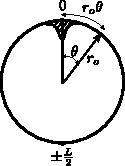
\includegraphics[width=0.2\textwidth]{1D_LP.pdf}
  \end{center}
\end{wrapfigure}
\
\
Let's continue with the example from the last class: 
\[r_o \theta = x, \quad x \in \left[\frac{-L}{2}, \frac{L}{2} \right]\]
\[\hat{H}_o = -\frac{\hbar^2}{2m}\frac{d^2}{dx^2}\]
\[\left(\text{B.C}\right):\quad \Psi_n\left(\frac{-L}{2}\right) =
  \Psi\left(\frac{L}{2}\right)
\]
Unperturbed eigenenergies and wavefunctions:
\[
  \mathcal{E}_n = \frac{2\hbar^2 \pi^2 n^2}{mL^2},\quad \Psi_n = e^{i 2\pi n \frac{x}{L}},
  \quad n \in \mathbb{Z}
\]\\
n can be positive or negative, to describe clockwise/counterclockwise motion around the ring, but 
$\mathcal{E}_{-n} = \mathcal{E}$, $n \neq 0$, so $\Psi_n$ is doubly degenerate for 
$n\neq 0$ ($\mathcal{E}\sim n^2$)\\
\\
\textbf{Check:}
\begin{align*}
  \big<\Psi_n\big|\Psi_n\big> &= A^2 \int_{-\frac{L}{2}}^{\frac{L}{2}} e^{-i2\pi n \frac{x}{L}}
  e^{i2\pi n \frac{x}{L}}dx = A^2 L = 1\\
 &= A^2\int_{-\frac{L}{2}}^{\frac{L}{2}} dx \\
 &\Rightarrow \boxed{A = \frac{1}{\sqrt{L}}}
\end{align*}
\begin{align*}
  \big<\Psi_{n'}\big|\Psi_n\big> &= \frac{1}{L}
   \int_{-\frac{L}{2}}^{\frac{L}{2}} e^{i2\pi(n-n') \frac{x}{L}}dx\\
  &= \frac{1}{L}\frac{L}{2i\pi (n-n') }e^{i2\pi(n-n') \frac{x}{L}}\Big|_{-\frac{L}{2}}^{\frac{L}{2}}\\
  &=\frac{L}{2i\pi (n-n') } \left(e^{i\pi(n-n')} -e^{-i\pi(n-n')}  \right)=0\\
  &= \frac{(-1)^{n-n'} - (-1)^{n-n'}}{2\pi(n-n')} = \begin{cases} 0,\quad n\neq n'\\ 
    1, \quad n = n'\\
  \end{cases}\\
  \big<\Psi_n\big|\Psi_n\big> &= \mathlarger{\delta}_{n'n}
\end{align*}
\subsection*{Perturbation}
\[
  \hat{V}' = -V_o\,e^{x^2/\Delta^2}, \quad \Delta \ll L
\]
A gaussian well centered @ $x=0$ is a "trap" for the particle, e.g. bent the wire @ $x=0$ that
forms the ring. \\
\\
For $n= 0$,
\[
  \Psi_0(x) = \frac{1}{\sqrt{L}}, \quad \text{in non-degenerate}
\]
\[
  \hat{ \tilde{H}} = \frac{-\hbar^2}{2m}\frac{d^2}{dx^2} - V_0\,e^{-x^2/\Delta^2}, \quad \text{
    we can use \emph{TINDPT} for
  }\,n=0
\]
\begin{align*}
  \tilde{\mathcal{E}}_0^{(1)} &=\big<\Psi_0\big|\hat{V}'\big|\Psi_0 \big> = \int_{-\frac{L}{2}}^
  {\frac{L}{2}}\left(\frac{1}{\sqrt{L}}\right)^2 \left(-V_0 e^{-x^2/\Delta^2}\right)dx\\
&= \frac{-V_0}{L}\int_{-\frac{L}{2}}^{\frac{L}{2}}\underbrace{e^{-x^2/\Delta^2}}_\text{even in x}\\
&=\frac{-2V_0}{L}\int_{0}^{\frac{L}{2}}e^{-x^2/\Delta^2} 
\end{align*}
Since $\Delta \ll L$, we can approximate the integral by extending the boundary to $\frac{L}{2}
\longrightarrow \infty$.
\begin{wrapfigure}{r}{4cm}
  \begin{center}
    \includegraphics[width=0.17\textwidth]{15.57.pdf}
  \end{center}
\end{wrapfigure}
\\Then, 
\[\mathcal{E}^{(1)}_0 = -\frac{2V_0}{L}\Bigg[\int_{0}^{\infty} e^{-x^2/\Delta^2} dx
- \underbrace{\int_{\frac{L}{2}}^{\infty}e^{-x^2/\Delta^2}}_{\text{negligeble for L}\gg\Delta}
\Bigg]\]\\
\[
  \boxed{\mathcal{E}_0^{(1)} = -\frac{V_0}{L}\sqrt{\pi}\Delta}\quad
  \fbox{%
  \parbox{.4\textwidth}{%
  \textbf{Recall:} We're using a perturbation theory, so all results are 
  approximate in any case.
  }%
}
\]
For $n\neq 0$, $\Psi_{\pm n}(x)$ are degenerate! use \emph{TIDPT}
\begin{align*}
  \mathcal{E}_{\pm n} &=\frac{W_{n,n} +W_{-n,-n}}{2} \pm 
  \sqrt{\left(\frac{W_{n,n}
  - W_{-n,-n}}{2}\right)^2 + \big|W_{n, -n}\big|^2},\quad\text{where } W_{n'n} = 
  \big<\psi_{n'}\big|\hat{V}'\big|\psi_n\big>\\
  W_{n,n}&= \int_{-L/2}^{L/2}\big|\psi_n(x)\big|^2\, \hat{V}'(x)dx = -\frac{V_0}{L}\int_{-L/2}
  ^{L/2}e^{-x^2/\Delta^2}e^{i2\pi n x/L}e^{-i2\pi n x/L}dx\\
         &= -2\frac{V_0}{L}\int_{0}^{L/2} e^{-x^2/\Delta}dx\\
         &\cong -2\frac{V_0}{L}\left(\frac{1}{2}\sqrt{\pi}\Delta\right) = \frac{-V_0}{L}\sqrt
         {\pi}\Delta, \quad\text{i.e. the \emph{TIDPT} is the same }\forall n\\
         &\Rightarrow \boxed{W_{n,n}= W_{-n,-n} = \frac{-V_0}{L}\sqrt{\pi}\Delta}
\end{align*}
$\mathbf{(\Delta \ll L)}$\\
\\
Since $W_{n,n} - W_{n,-n} = 0$
\[\mathcal{E}_{\pm n} = \frac{-V_0}{L}\sqrt{\pi}\Delta \,\pm\, \big|W_{n,-n}\big|\]
\[W_{n,-n} = \frac{-V_0}{L}\int_{-L/2}^{L/2} e^{-x^2/\Delta^2} e^{i4\pi n x/L} dx\]
We will use:
\begin{equation}
\boxed{ \int_{-\infty}^{+\infty}e^{-(ax^2+bx+c)}dx = \sqrt{\frac{\pi}{a}}\,e^{\frac{b^2-4ac}{4a}} }
\end{equation}
\begin{align*}
  \mathcal{E}_{\pm n} &= \frac{V_0}{L}\sqrt{\pi}\Delta\,\,\pm\frac{-V_0}{L}\sqrt{\pi}\Delta\,
  e^{-(2\pi n \Delta/L)^2}\\
                      &= \boxed{\frac{-V_0}{L}\sqrt{\pi}\Delta\left(1 \pm e^{-\left(
                      \frac{2\pi n \Delta}{L}\right)^2}\right) }
\end{align*}
\textbf{Alternatively:} $V'(x) = -V_0 e^{-x^2/\Delta^2}$ is an even function of $x$, so, if
our wavefunction, i.e. linear combinations of $\Psi_n$ and $\Psi_{-n}$ were even/odd, they would 
be eigenfunction of the perturbation!\\
\\
Even part of $\Psi_n(x):$
\[
  \frac{\psi_n(x)+\psi_n(-x)}{2} = \frac{e^{i2\pi n x/L + e^{-i2\pi n x/L}}}{2\sqrt{L}}=
\frac{1}{\sqrt{L}}Cos\left(\frac{2\pi n x}{L}\right)
\]
Odd part of $\Psi_n(x):$
\[
   \frac{\psi_n(x)-\psi_n(-x)}{2} = \frac{e^{i2\pi n x/L - e^{-i2\pi n x/L}}}{2\sqrt{L}}=
   \frac{\psi_n(x)}{2}-\frac{\psi_{-n}(x)}{2}=
\frac{i}{\sqrt{L}}Sin\left(\frac{2\pi n x}{L}\right)
\]
\begin{align*}
  W_{\alpha\beta}&=\Bigg<\frac{i}{\sqrt{\pi}}Sin\left(\frac{2\pi n x}{L}\right)\Bigg| V_0 e^{
  -x^2/\Delta^2}\Bigg|\frac{1}{\sqrt{L}}Cos\left(\frac{2\pi n x}{L}\right)\Bigg>\\
                 &= \frac{-iV_0}{L}\int_{-L/2}^{L/2}\underbrace{\underbrace{Sin\left(\frac{2\pi n x}
                 {L}\right)}_\text{odd}
\underbrace{ Cos\left(\frac{2\pi n x}{L}\right)}_\text{even} \underbrace{e^{-x^2/\Delta^2
}}_\text{even}}_\text{odd} dx = 0
  \end{align*}
Sine and Cosine are eigenfunctions of the perturbation.
\begin{align*}
  W_{\alpha\alpha} &= \int_{-L/2}^{L/2}Cos^2\left(\frac{2\pi n x}{L}\right)\left(
  \frac{-V_0}{L}\right)e^{-x^2/\Delta^2} dx\\
  &= \frac{-2V_0}{L}\int_{0}^{L/2} Cos^2\left(\frac{2\pi n x}{L}\right) e^{-x^2/\Delta^2}dx
  \end{align*}
Professor made a bunch of mistakes here, so tried to correct them using other approach, but as 
you may have noticed, we corrected them, and it is not necessary to introduce Sines and Cosines.
Anyway, in the next lecture he sure will correct this problem and shows us a plot of the 
eigenenergies.
%%%%%%%%%%%%%%%%%%%%%%%%%%%%%%%%%%%%%%%%%%%%%%%%%%%%%%%%%%%%%%%%%%%%%%%%%%%%%%%%%%%%%%%%%%%%%%%%
%%%%%%%%%%%%%%%%%%%%%%%%%%%%%%%%%%%%%%%%%%%%%%%%%%%%%%%%%%%%%%%%%%%%%%%%%%%%%%%%%%%%%%%%%%%%%%%%
%%%%%%%%%%%%%%%%%%%%%%%%%%%%%%%%%%%%%%%%%%%%%%%%%%%%%%%%%%%%%%%%%%%%%%%%%%%%%%%%%%%%%%%%%%%%%%%%
%%%%%%%%%%%%%%%%%%%%%%%%%%%%%%%%%%%%%%%%%%%%%%%%%%%%%%%%%%%%%%%%%%%%%%%%%%%%%%%%%%%%%%%%%%%%%%%%
\newpage
\section{Lecture 11}
May 17, 2023
\begin{empheq}[box=\fbox]{align*}
  \psi_n(x) &= \frac{1}{\sqrt{L}}e^{2i\pi x/L}\\
  \mathcal{E}_n &= \frac{2\hbar^2 \pi^2 n^2}{mL^2}\\
  \hat{V}(x) &= -V_0 e^{-x^2/\Delta^2}
\end{empheq}
We will use:
\begin{equation}
\boxed{ \int_{-\infty}^{+\infty}e^{ax^2+bx+c}dx = \sqrt{\frac{\pi}{a}}\,e^{\frac{b^2-4ac}{4a}} }
\end{equation}
\begin{align*}
  W_{nn} &= \big<\psi_n\big|\hat{V}\big|\psi_n\big>\\
  &= \frac{-V_0}{L}\int_{-\frac{L}{2}}^{\frac{L}{2}}\cancelto{1}{\bigg|e^{2\pi i nx/L}\bigg|^2}
  e^{-x^2/\Delta^2}dx
\end{align*}
then, following (3.5.1):
\[a=\frac{1}{\Delta^2}, \quad b = 0, \quad c=0\]
\[\boxed{=\frac{-V_0}{L}\sqrt{\pi}\Delta = -\sqrt{\pi}V_0 \frac{\Delta}{L},\quad \Delta\ll L}\]
\\
\[
  W_{n,-n} = \frac{-V_0}{L}\int_{-\frac{L}{2}}^{\frac{L}{2}} e^{4\pi i n x/L}e^{-x^2/\Delta^2}dx
\]
\[
  a = \frac{1}{\Delta^2}, \quad b = 4\pi i n/L, \quad c=0,\quad \text{Let}\,L\longrightarrow 
  \infty
\]
Then, 
\[
  W_{n,-n} = \frac{-V_0}{L}e^{\frac{-16\pi^2 n^2 \Delta^2}{4L^2}} = \frac{-V_0}{L}\sqrt{\pi}\Delta
  e^{-\left(\frac{2\pi n \Delta}{L}\right)^2}
\]
\[\Rightarrow \boxed{\tilde{\mathcal{E}}_{\pm n}^{(1)}= \frac{-V_0\sqrt{\pi}\Delta}{L}\left(
1\,\pm\,  e^{-\left(\frac{2\pi n \Delta}{L}\right)^2}\right)}\]
\newpage 
\begin{wrapfigure}{l}{8cm}
  \begin{center}
    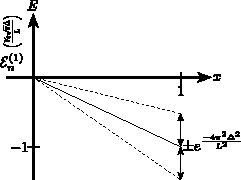
\includegraphics[width=0.4\textwidth, height=5cm]{F11.pdf}
  \end{center}
\end{wrapfigure}
\
\
\
\noindent
Splitting around $ \frac{-V_0\sqrt{\pi}\Delta}{L} $ of
$ e^{-\left(\frac{2\pi n \Delta}{L}\right)^2} $, so the strongest effect is for:
\begin{align*}
  n &= 1: \pm e^{\frac{-4\pi^2\Delta^2}{L^2}}\\
  n &= 2:\pm e^{\frac{-16\pi^2\Delta^2}{L^2}}\\
  n &= 3: \pm e^{\frac{-32\pi^2\Delta^2}{L^2}}\quad (\text{very small!})
\end{align*}
i.e. splitting is significant only for $n=1$ , (and 2), remember  $\Delta\ll L$, so 
$\Delta^2/L^2 \ll 1$, so $\frac{4\pi^2 n^2 \Delta^2}{L^2}\gg 1 \Leftrightarrow n\gg\frac{L}
{2\pi\Delta}$ for the splitting to be negligible.
\noindent
\textbf{Consider the k-fold degenerate state}
\\
\begin{equation} 
  \begin{pmatrix} 
    W_{n,n} & \dots  &  W_{n,n+k-1}\\
    \vdots & \ddots & \vdots\\
    W_{n+k-1} & \dots  &  
    W_{n+k-1,n+k-1} 
    \end{pmatrix}
    \begin{pmatrix}
      C_n\\
      \vdots\\
      C_{n+k-1}
    \end{pmatrix}
    = \mathcal{E}
    \begin{pmatrix}
  C_n\\
      \vdots\\
      C_{n+k-1}
    \end{pmatrix}
  \end{equation}
  \\
  where $C_{n'} = \big<\psi_{n'}\big|\tilde{\psi}^{(0)} \big>$ are the coefficients  of the Zeroth
  order eigenstate of the perturbation in the basis of the unperturbed hamiltonian's k-fold degenerate
  eigenstates, where $\hat{H}_0\big|\psi_{n'}\big> = \mathcal{E}\big|\psi_{n'}\big>\quad \forall 
  n' \in \{n, \cdots, n+k-1 \}$\\
  \\
  \textbf{Recall:} $W_{n'n} = \big<\tilde{\Psi}_{n'}\big|\hat{V}'\big|\tilde{\Psi}_n \big>$, are
  the matrix elements for the perturbation in this basis.
\subsection*{Idea}
\{$\Psi_n, \cdots, \Psi_{n+k-1} $\} forms an orthogonal basis which spans the space of the states 
with unperturbed eigenenergies $\mathcal{E}$.\\
You can express any eigenstate of the perturbation with unperturbed eigenenergy $\mathcal{E}$
as a linear combination of the k-fold degenerate eigenstates of the unperturbed hamiltonian 
$\hat{H}_0$. \\
\\
\textbf{Want:}
\[
  \big<\tilde{\Psi}^{(0)}\big|\hat{V}\big|\tilde{\Psi}^{(0)}\big> = \tilde{\mathcal{E}}^{(1)}
\]
So, $\hat{V}\big|\tilde{\Psi}^{(0)}\big> = \tilde{\mathcal{E}}^{(1)}\big|\tilde{\Psi}^{(0)}\big>$
, since it spans the the space:
\[
  \sum_{n'n''=n}^{n+k-1}\big|\psi_{n'}\big>\big<\psi_{n'}\big| =
  \sum_{n'=n}^{n+k-1}\big|\psi_{n'}\big>\big<\psi_{n'}\big| = \mathbb{1}
\]
\[
  \hat{V}\sum_{n'n''=n}^{n+k-1}\big|\psi_{n'}\big>\big<\psi_{n'}\big|\tilde{\psi}^{(0)}\big> =
  \tilde{\mathcal{E}}^{(1)} \sum_{n'=n}^{n+k-1}\big|\psi_{n'}\big>\underbrace{\big<\psi_{n'}
  \big|\tilde{\psi}^{(0)}\big>}_{C_{n'}} = 
  \mathbb{1} 
\]
Multiply by $\big<\psi_{n'}\big|$:
\[
  \sum_{n'=n}^{n+k-1} \big<\psi_{n''}\big|\hat{V}\big|\psi_{n'}\big>C_{n'} = 
  \tilde{\mathcal{E}}^{(1)}\sum_{n'}\mathlarger{\delta}_{n''n}C_{n'} = \tilde{\mathcal{E}}^{(1)}
  C_{n'}
\]
\\
\textbf{For k = 2:}
\\
\begin{equation}
  \begin{pmatrix}
  W_{nn} & W_{n,n+1}\\
  W_{n+1, n} & W_{n+1, n+1}
  \end{pmatrix}
  \begin{pmatrix}
  C_n\\
  C_{n+1}
\end{pmatrix}= \tilde{\mathcal{E}}^{(1)}
\begin{pmatrix}
  C_{n}\\
  C_{n+1}
\end{pmatrix}
\end{equation}
\\
\begin{equation}
  W_{n+1,n}C_{n}  + W_{n,n+1}C_{n+1} = \tilde{\mathcal{E}}^{(1)}C_{n} \Longrightarrow C_{n+1} =
  \left(\frac{\tilde{\mathcal{E}}^{(1)}-W_{nn}}{W_{n,n+1}}\right)C_n
\end{equation}
\[
  W_{n+1,n}C_n + W_{n+1,n+1}C_{n+1} = \tilde{\mathcal{E}}^{(1)}C_{n+1},\quad\text{substitute
  here (3.5.4)}
\]
\[
  C_n\left( W_{n+1,n} + W_{n+1, n+1}\left(\frac{\tilde{\mathcal{E}}^{(1)}-W_{n,n}}{W_{n,n+1}}
  \right)-\tilde{\mathcal{E}}^{(1)}\left(\frac{\tilde{\mathcal{E}}^{(1)}-W_{nn}}
{W_{n,n+1}}\right) \right) = 0
\]
if $C_n\neq 0$: multiply $W_{n,n+1}$ and get:
\[
  W_{n+1,n}W_{n,n+1}+\left(W_{n+1, n+1}+W_{nn} \right)\tilde{\mathcal{E}}^{(1)} - W_{n+1, n+1}
  W_{nn}-\tilde{\mathcal{E}}^{(1)2}=0
\]
\[
  \tilde{\mathcal{E}}^{(1)2} - \left(W_{nn}+W_{n+1,n+1} \right) \tilde{\mathcal{E}}^{(1)} + 
  W_{nn}W_{n+1,n+1} - \big|W_{n,n+1}\big|^2 = 0
\]
\begin{equation}
  \boxed{\tilde{\mathcal{E}}^{(1)} = \frac{W_{nn}+W_{n+1,n+1}}{2}\,\pm\, \sqrt{
      \left(\frac{W_{nn} - W_{n+1,n+1}}{2}\right)^2 + \big|W_{n,n+1}\big|^2
  }}
\end{equation}
\\
\begin{equation}
  det\left(W - \tilde{\mathcal{E}}^{(1)}\mathbb{1} \right)=0
\end{equation}
\begin{align*}
  \left(W_{nn}- \mathcal{E}\right)\left(W_{n+1,n+1} - \mathcal{E}\right) - W_{n,n+1}W_{n+1,n} &=0\\
  \mathcal{E}^2 - \left(W_{nn}+W_{n+1,n+1}\right)\mathcal{E}+W_{nn}W_{n+1,n+1}-\big|W_{n,n+1}
  \big|^2 &= 0
\end{align*}
\begin{equation}
  \boxed{\mathcal{E}_\pm = \frac{W_{nn}+W_{n+1,n+1}}{2}\,\pm\, \sqrt{
      \left(\frac{W_{nn} - W_{n+1,n+1}}{2}\right)^2 + \big|W_{n,n+1}\big|^2
  }}
\end{equation}
\subsection{Example}
\begin{wrapfigure}{l}{6cm}
  \begin{center}
    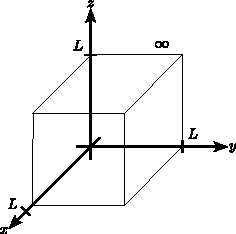
\includegraphics[width=0.35\textwidth]{3DSW.pdf}
  \end{center}
\end{wrapfigure}
Consider a 3D infinite cubic square well of dimension $L$
\begin{equation}
  V_\infty(x,y,z) = 
  \begin{cases}
    0,& \quad\text{for}\,\,\, 0\leq x,y,z \leq L\\
    \infty, &\quad \text{otherwise}
  \end{cases}
\end{equation}
\[
\hat{H}_0 = \frac{-\hbar^2}{2m}\nabla^2 \Rightarrow \]
\[
(TISE):\quad \frac{-\hbar^2}{2m}\nabla^2\Psi
  (x,y,z) = \mathcal{E}\Psi(x,y,z)
\]
\[
  \frac{\partial^2\Psi}{\partial x^2}+ \frac{\partial^2\Psi}{\partial y^2}+
  \frac{\partial^2\Psi}{\partial z^2} = \frac{-2m\mathcal{E}}{\hbar^2}
\]
Assume $\Psi(x,y,z) = X(x)Y(y)Z(z)$:
\[
  \frac{X''(x)}{X(x)}+ \frac{Y''(y)}{Y(y)}+ \frac{Z''(z)}{Z(z)} = \frac{-2m\mathcal{E}}{\hbar^2}
\]
\[
  \frac{X''(x)}{X(x)} = \frac{-2m\mathcal{E}}{\hbar^2}-\left(\frac{Y''(y)}{Y(y)}+
  \frac{Z''(z)}{Z(z)}\right) = -\lambda_x = \frac{-n^2_x \pi^2}{L^2}
\]
\[
  X''(x) = -\lambda_x X(x) \Rightarrow X(x) = A\,Cos\left(\sqrt{\lambda_x}x\right)+
  B\,Sin\left(\sqrt{\lambda_x}x\right)
\]
(B.C):
\[
  X(0) = X(L) = 0 \Rightarrow X(0) = \boxed{A = 0}, 
  \quad X(L) = B\,Sin\left(\sqrt{\lambda_x}x\right) = 0
\]
\[
  (B\neq 0) \Rightarrow \sqrt{\lambda_x}L = n_x \pi,\quad n_x \in \mathbb{N}\quad
    \fbox{%
  \parbox{.4\textwidth}{%
    $-n$ gives the same $X_{-n}(x) = -X(x)$ up to a factor of $-1$ so no linearly independent.
    $n_x=0\Rightarrow$ no particle, empty state.
  }%
}
\]
\[
  \Rightarrow \boxed{\lambda_x = \frac{n^2_x\pi^2}{L^2}}
\]
\begin{empheq}[box=\fbox]{align}
  X(x) &= B_x\,Sin\left(\frac{n_x\pi x}{L}\right)\\
   Y(y) &= B_y\,Sin\left(\frac{n_y\pi y}{L}\right)\\
  Z(z) &= B_z\,Sin\left(\frac{n_z\pi z}{L}\right)
\end{empheq}
\begin{equation}
  \frac{-2m\mathcal{E}}{\hbar^2} = \lambda_x - \lambda_y - \lambda_z = \frac{\pi^2}{L^2}
  \left(n_x^2 + n_y^2 + n_z^2 \right) \Rightarrow \boxed{\mathcal{E}_{n_x,n_y,n_z} = \frac{\pi^2 \hbar^2}
  {2mL^2}
\left(n_x^2 + n_y^2 + n_z^2\right)}
\end{equation}
\begin{equation}
  \boxed{\Psi_{n_x,n_y,n_z} = B_xB_yB_z\,Sin\left(\frac{n_x \pi x}{L}\right)
  Sin\left(\frac{n_y \pi y}{L}\right)Sin\left(\frac{n_z \pi z}{L}\right)}
\end{equation}
\\
Now, we need to find $B_xB_yB_z$:
\\
\begin{align*}
  \big<\Psi_{n'_x,n'_y,n'_z}\big|\Psi_{n_x,n_y,n_z} \big>& =B^2_xB^2_yB^2_z \int_{0}^{L}
  Sin\left(\frac{n'_x \pi x}{L}\right)Sin\left(\frac{n_x \pi x}{L}\right)dx\\
  & \cdot\int_{0}^{L}
  Sin\left(\frac{n'_y \pi y}{L}\right)Sin\left(\frac{n_y \pi y}{L}\right)dy\\
  & \cdot\int_{0}^{L}
  Sin\left(\frac{n'_z \pi z}{L}\right)Sin\left(\frac{n_z \pi z}{L}\right)dz\\
  &=B^2_xB^2_yB^2_z \left(\mathlarger{\delta}_{n'_x,n_x}\frac{L}{2}\right)
  \left(\mathlarger{\delta}_{n'_y,n_y}\frac{L}{2}\right)
  \left(\mathlarger{\delta}_{n'_z,n_z}\frac{L}{2}\right)
\end{align*}
\[
  \Rightarrow B_x = B_y = B_z = \sqrt{\frac{2}{L}}
\]
\begin{equation}
  \boxed{\Psi_{n_x,n_y,n_z} = \left(\frac{2}{L}\right)^{3/2}\,Sin\left(\frac{n_x \pi x}{L}\right)
  Sin\left(\frac{n_y \pi y}{L}\right)Sin\left(\frac{n_z \pi z}{L}\right) }
\end{equation}
\\
Then, \\
\[
  \Psi_{111}(x,y,z) =\left(\frac{2}{L}\right)^{3/2}\,Sin\left(\frac{\pi x}{L}\right)
  Sin\left(\frac{ \pi y}{L}\right)Sin\left(\frac{ \pi z}{L}\right) 
\]
\[
  \mathcal{E}_{111} = \frac{\pi^2 \hbar^2}{2mL^2}(1+1+1) =\frac{3\pi \hbar^2}{2mL^2}\quad
   \fbox{%
  \parbox{.2\textwidth}{%
    (ground state)\\
  non-degenerate}%
}
\]
\textbf{$1^{st}$ excited state:}
\[
  \mathcal{E}_{211} = \mathcal{E}_{121} = \mathcal{E}_{112} = \frac{\pi^2 \hbar^2}{2mL^2}(1+1+4)
  = \frac{3\pi^2 \hbar^2}{mL^2}\quad \fbox {%
    \parbox{.15\textwidth}{%
three-fold \\
degenerate}%
}
\]
Now, let's introduce a perturbation:\\
\newpage

\begin{wrapfigure}[15]{l}{7cm}
  \begin{center}
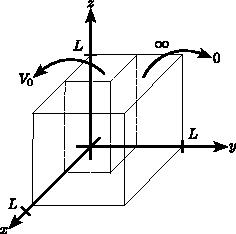
\includegraphics[width=0.35\textwidth]{3DPE.pdf}
  \end{center}
\end{wrapfigure}
\begin{align*}
  \hat{V}'(x,y)&=\begin{cases}
    V_0 &,\quad \text{for} 0\leq x,y \leq L/2\\
    0&, \quad \text{otherwise}
  \end{cases}\\
    V'(x,y) &= V_0\left(1-\Theta\left(x-\frac{L}{2}\right) \Theta\left(y-\frac{L}{2}\right)\right)\\
            &= V_0\left(\Theta\left(x-\frac{L}{2}\right) \Theta\left(y-\frac{L}{2}\right) \right)
\end{align*}
\qquad \qquad \qquad\qquad \qquad \qquad \qquad\qquad\qquad   where: 
\[
 \qquad\qquad\qquad\qquad \Theta(x) = 
  \begin{cases}
    1 &,\quad x\geq 0\\
    0 &,\quad x \leq 0
  \end{cases}
\]
\qquad \qquad \qquad\qquad \qquad \qquad \qquad\qquad\qquad is the Heaviside step function.\\
\textbf{Ground State:}
\begin{align*}
  \tilde{\mathcal{E}}_{111}^{(1)} &= \big<\Psi_{111}\big|\hat{V}'\big|\Psi_{111} \big>\quad
  \text{(\emph{TINDPT})}\\
&= \int_{0}^{L}\int_{0}^{L}\int_{0}^{L}\left(\frac{2}{L}\right)\,Sin^2\left(\frac{\pi x}{L}\right)
  Sin^2\left(\frac{ \pi y}{L}\right)Sin^2\left(\frac{ \pi z}{L}\right)
  V_0\Theta\left(x-\frac{L}{2}\right) \Theta\left(y-\frac{L}{2}\right)dxdydz\\
&= \frac{8V_0}{L^3}\int_{0}^{L/2}\,Sin^2\left(\frac{\pi x}{L}\right)dx
\int_{0}^{L/2}\,Sin^2\left(\frac{\pi y}{L}\right)dy
\int_{0}^{L}\,Sin^2\left(\frac{\pi z}{L}\right)dz\\
&= \frac{8V_0}{L^3}\left(\frac{L}{4}\right)\left(\frac{L}{4}\right)\left(\frac{L}{2}\right)
=\frac{V_0}{4}  \quad \fbox{%
  \parbox{.2\textwidth}{%
    $V_0$ acts on a quarter of the well.}%
  }
\end{align*}
\begin{align*}
  \Psi_{211}(x,y,z) &= \left(\frac{2}{L}\right)^{3/2}\,Sin\left(\frac{2\pi x}{L}\right)Sin\left(
  \frac{\pi y}{L}\right)Sin\left(\frac{\pi z}{L}\right)\\
\Psi_{121}(x,y,z) &= \left(\frac{2}{L}\right)^{3/2}\,Sin\left(\frac{\pi x}{L}\right)Sin\left(
  \frac{2\pi y}{L}\right)Sin\left(\frac{\pi z}{L}\right)\\
  \Psi_{112}(x,y,z) &= \left(\frac{2}{L}\right)^{3/2}\,Sin\left(\frac{\pi x}{L}\right)Sin\left(
  \frac{\pi y}{L}\right)Sin\left(\frac{2\pi z}{L}\right)
\end{align*}
\begin{align*}
  \big<\Psi_{211}\big|\hat{V}'\big|\Psi_{211}\big> &= \left(\frac{2}{L}\right)^{3}\,
  \int_{0}^{L/2} Sin^2\left(\frac{2\pi x}{L}\right)dx\int_{0}^{L/2}Sin^2\left(\frac{\pi y}{L}
  \right)dy\int_{0}^{L}Sin^2\left(\frac{\pi z}{L}\right)dz\\
  &= \frac{8V_0}{L}\left(\frac{L}{4}\right)\left(\frac{L}{4}\right)\left(\frac{L}{2}\right)
  = \frac{V_0}{4}= \big<\Psi_{121}\big|\hat{V}'\big|\Psi_{121}\big>
\end{align*}
\begin{align*}
\big<\Psi_{211}\big|\hat{V}'\big|\Psi_{121}\big> &=\left(\frac{2}{L}\right)^{3}
\int_{0}^{\frac{L}{2}} Sin\left(\frac{\pi x}{L}\right)Sin\left(\frac{2\pi x}{L}\right)dx
\int_{0}^{\frac{L}{2}}Sin\left(\frac{2\pi y}{L}\right)Sin\left(\frac{\pi x}{L}\right) dy
\int_{0}^{L}\cancelto{L/2}{Sin^2\left(\frac{\pi z}{L}\right)}dz
\end{align*}
Using
\[
  \boxed{Sin(A)Sin(B) = \frac{1}{2}\left(Cos(A-B)- Cos(A+B)\right)}
\]
\begin{align*}
 \big<\Psi_{211}\big|\hat{V}'\big|\Psi_{121}\big> 
 &= \big<\Psi_{121}\big|\hat{V}'\big|\Psi_{211}\big> = \frac{4V_0}{L^2}\left[\int_{0}^{\frac{L}{2}
 }\left(Cos\left(\frac{\pi x}{L}\right) \right)-Cos\left(\frac{3\pi x}{L} \right)dx \right]^2\\
 &= \frac{V_0}{L^2}\left[\left(\frac{L}{\pi}Sin\left(\frac{\pi x}{L}\right) - \frac{L}{3\pi}
 Sin\left(\frac{3\pi x}{L}\right)\right)\Bigg|_{0}^{L/2}\right]^2\\
 &= \frac{V_0}{L^2}\frac{L^2}{\pi^2}\left[1 - \frac{(-1)}{3}\right]^2\\
 &= \frac{16V_0}{9\pi^2} = \left(\frac{8}{3\pi}\right)^2 \frac{V_0}{4},\quad\text{let }\,\, k =
 \frac{8}{3\pi}
\end{align*}
Note:
\[
  \frac{2}{L}\int_{0}^{L}Sin\left(\frac{2\pi z}{L}\right)Sin\left(\frac{\pi z}{L}\right)dz =
  \mathlarger{\delta}_{21}=0
\]
Finally, we have that:
\begin{equation}
  \mathcal{W}=
  \begin{pmatrix}
    \frac{V_0}{4} & \frac{V_0}{4} k^2 & 0\\
    \frac{V_0}{4} k^2 & \frac{V_0}{4} & 0\\
    0 & 0 & \frac{V_0}{4}
  \end{pmatrix} =
  \frac{V_0}{4}
  \begin{pmatrix}
    1 & k^2 & 0\\
    k^2 & 1 & 0\\
    0 & 0 & 1
  \end{pmatrix}
\end{equation}
\begin{align*}
  &\left(1-\mathcal{E}\right)\left(\left(1-\mathcal{E}\right)^2 - k^2\right) =0 \\
  & \Rightarrow \mathcal{E} = 1\\
  & \Rightarrow \mathcal{E} = 1 \pm \sqrt{1 - 4(1-k)^2}
\end{align*}
\newpage
\clearpage
%%%%%%%%%%%%%%%%%%%%%%%%%%%%%%%%%%%%%%%%%%%%%%%%%%%%%%%%%%%%%%%%%%%%%%%%%%%%%%%%%%%%%%%%%%%%%%
%%%%%%%%%%%%%%%%%%%%%%%%%%%%%%%%%%%%%%%%%%%%%%%%%%%%%%%%%%%%%%%%%%%%%%%%%%%%%%%%%%%%%%%%%%%%%%
%%%%%%%%%%%%%%%%%%%%%%%%%%%%%%%%%%%%%%%%%%%%%%%%%%%%%%%%%%%%%%%%%%%%%%%%%%%%%%%%%%%%%%%%%%%%%%
%%%%%%%%%%%%%%%%%%%%%%%%%%%%%%%%%%%%%%%%%%%%%%%%%%%%%%%%%%%%%%%%%%%%%%%%%%%%%%%%%%%%%%%%%%%%%%
%%%%%%%%%%%%%%%%%%%%%%%%%%%%%%%%%%%%%%%%%%%%%%%%%%%%%%%%%%%%%%%%%%%%%%%%%%%%%%%%%%%%%%%%%%%%%%
\section{Lecture 12}
May 22, 2023
\subsection*{Example}
3D infinite square well
\begin{align*}
  E_{n_x,n_y,n_z} &= \frac{\pi^2 \hbar^2}{2mL^2}\left(n_x^2+n_y^2+n_z^2 \right)\\
  \Psi_{n_x,n_y,n_z} &= \left(\frac{2}{L}\right)^{3/2}\,Sin\left(\frac{n_x \pi x}{L}\right)
  Sin\left(\frac{n_y \pi y}{L}\right)Sin\left(\frac{n_z \pi z}{L}\right) \\
  \hat{V}'&= V_0\left(\Theta\left(x-\frac{L}{2}\right) \Theta\left(y-\frac{L}{2}\right) \right)
\end{align*}
\[
  \underbrace{W_{n_xn_yn_z,n'_xn'_yn'_z}}_{W-\text{matrix}} =\underbrace{\big< \Psi_{n_x,n_y,n_z}
  \big|\hat{V}'\big|
\Psi_{n'_x,n'_y,n'_z} \big>}_{\text{matrix elements}}
\]
\[
  W_{211,211} = W_{121,121} = W_{112,112} = \frac{V_0}{4} 
\]
\[
  W_{211,121} = W_{121,211}^* = \frac{V_0}{4}\left(\frac{8}{3\pi}\right)^2 = \frac{V_0}{4}k^2
\]
\[
  \frac{2}{L}\int_{0}^{L}Sin\left(\frac{2\pi z}{L}\right)Sin\left(\frac{\pi z}{L}\right)dz =
  \mathlarger{\delta}_{21}=0
\]
if $n'_z = 2, n_z = 1, W_{n_xn_y1,n'_xn'_y2} = 0, \quad \forall\, n_x,n_y,n'_x,n'_y \in \mathbb{N}$
\begin{equation}
  \mathcal{W}=
 \frac{V_0}{4}
  \begin{pmatrix}
    1 & k^2 & 0\\
    k^2 & 1 & 0\\
    0 & 0 & 1
  \end{pmatrix}
  \begin{pmatrix}
    \alpha\\
    \beta\\
    \gamma
  \end{pmatrix} = \tilde{\mathcal{E}}^{(1)}
  \begin{pmatrix}
    \alpha\\
    \beta\\
    \gamma\\
  \end{pmatrix}
\end{equation}
To solve for $\tilde{\mathcal{E}}^{(1)}$, the first order corrections to $E_{211} =E_{121}
=E_{112} = \frac{3\pi^2 \hbar^2}{mL^2}$ let $\tilde{\mathcal{E}}^{(1)} = \frac{V_0}{4}\omega$
\[
  \text{det}
  \begin{pmatrix}
  1-\omega & k^2 & 0\\
  k^2 & 1-\omega & 0\\
  0 & 0 & 1-\omega
  \end{pmatrix}
  = 0
\]
\[
  (1-\omega)\,\text{det}
  \begin{pmatrix}
    1-\omega & k^2\\
    k^2 & 1-\omega
  \end{pmatrix}
  = 0
\]
\[
  (1-\omega)\left((1-\omega)^2 - k^4\right) = 0
\]
\begin{wrapfigure}{l}{7cm}
  \begin{center}
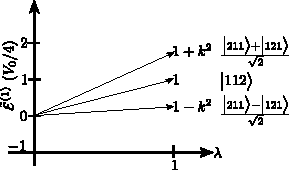
\includegraphics[width=0.4\textwidth]{EN3.pdf}
  \end{center}
\end{wrapfigure}
\
\
Solutions:
\begin{align*}
  \hat{\omega} &= 1\\
  \hat{\omega} & = 1 \pm k^2
\end{align*}
\begin{equation}
  \tilde{\mathcal{E}}^{(1)} = 
  \begin{cases}
  \frac{V_0}{4}\\
  \frac{V_0}{4}\left(1+\left(\frac{8}{3\pi}\right)^2\right)\\
\frac{V_0}{4}\left(1-\left(\frac{8}{3\pi}\right)^2\right)
\end{cases}
\end{equation}
\[
 = \frac{V_0}{4}
 \begin{cases}
  0.28\\
  1.00\\
  1.72
  \end{cases}
\]
Solve for the eigenstates of $\hat{V}'$ in {$ \big|211\big>, \big|121\big>, \big|112\big>$} basis:\\
\\
\textbf{Method:} Substitute the eigenenergies into (3.6.1)  and solve for the coefficients 
$\alpha, \beta, \gamma $
\begin{align*}
  \tilde{\mathcal{E}}^{(1)} = \frac{V_0}{4}:  \quad \alpha + k^2 \beta = \alpha &\Rightarrow \beta=0\\
  \quad k^2\alpha+\beta = \beta &\Rightarrow \alpha = 0\quad \Rightarrow \fbox{%
  \parbox{.2\textwidth}{%
  $\big|112\big>$ is the eigenstate with energy $V_0/4$}%
}\\
  \gamma = \gamma & \Rightarrow \big|\gamma\big|^2 = 1
\end{align*}
\begin{align*}
  \tilde{\mathcal{E}}^{(1)}= \frac{V_0}{4}\left(1+k^2\right): \quad 
  \alpha +k^2\beta &= \left(1+k^2\right)\alpha\\
  k^2\beta = k^2\alpha &\Rightarrow \alpha=\beta\\
  k^2\alpha+\beta =\left(1+k^2\right)\beta& \Rightarrow \alpha = \beta\\
  \gamma = k^2\gamma &\Rightarrow \gamma = 0
\end{align*}
Normalisation: $\big|\alpha\big|^2 + \big|\alpha\big|^2 = 1 \Rightarrow \alpha = \frac{1}{
\sqrt{2}} = \beta$
\[
  \Rightarrow \frac{\big|211\big>+\big|121\big>}{\sqrt{2}}\quad \fbox{%
  \parbox{.2\textwidth}{%
  is the eigenstate with energy $V_0/4 (1+k^2)$}%
} 
\]
\begin{align*}
  \tilde{\mathcal{E}}^{(1)} = \frac{V_0}{4}\left(1+k^2\right):\quad \alpha +\beta k^2 = 
  \left(1-k^2\right)\alpha &\Rightarrow \alpha = -\beta\\
  k^2\alpha +\beta  = \left(1-k^2\right)\beta &\Rightarrow \alpha = \beta\\
  \gamma = \left(1-k^2\right)\gamma &\Rightarrow \gamma = 0
\end{align*}
\newpage
\clearpage
Normalisation: $\big|\alpha\big|^2 + \big|\beta\big|^2+\big|\gamma\big|^2 = 2\big|\alpha\big|^2=
1 \Rightarrow \alpha = \frac{1}{\sqrt{2}}\quad \text{and}\quad \beta=\frac{-1}{\sqrt{2}}$.\\
\[
  \Rightarrow \frac{\big|211\big>-\big|121\big>}{\sqrt{2}}\quad \fbox{%
  \parbox{.2\textwidth}{%
  is the eigenstate with energy $V_0/4 (1-k^2)$}%
} 
\]
\subsection*{Example}
\begin{wrapfigure}[5]{l}{7cm}
  \begin{center}
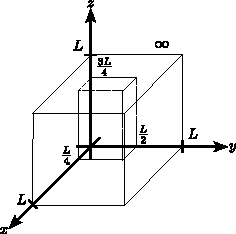
\includegraphics[width=0.35\textwidth]{BOX4.pdf}
  \end{center}
\end{wrapfigure}
\
\
Now: $\hat{V} = L^3V_0 \mathlarger{\delta}\left(x-\frac{L}{4}\right)
\mathlarger{\delta}\left(y-\frac{L}{2}\right)
\mathlarger{\delta}\left(z-\frac{3L}{4}\right)$\\
\\
$\mathlarger{\delta}$ "bump" @ $\left(\frac{L}{4}, \frac{L}{2}, \frac{3L}{4}\right)$
\begin{align*}
  \tilde{\mathcal{E}}_{111}^{(1)} &= \big<111\big|\hat{V}'\big|111 \big>, \quad \text{Since}\,
  \big|111\big>\, \text{is non-degenerate}\\
  &= \left(\frac{2}{L}\right)^3\int_{0}^{L}\int_{0}^{L}
  \int_{0}^{L}Sin^2\left(\frac{\pi x}{L}\right)Sin^2\left(\frac{\pi y}{L}\right)Sin^2
  \left(\frac{\pi z}{L}\right)\\
   &\mathlarger{\delta}\left(x-\frac{L}{4}\right)
\mathlarger{\delta}\left(y-\frac{L}{2}\right)
\mathlarger{\delta}\left(z-\frac{3L}{4}\right)dxdydz\\
&= V_0\,8\,Sin^2\left(\frac{\pi}{4}\right)Sin^2\left(\frac{\pi}{2}\right)
Sin^2\left(\frac{3\pi}{4}\right)\\
&= 8\,V_0\left(\frac{1}{\sqrt{2}}\right)^2 (1) \left(\frac{-1}{\sqrt{2}}\right)\\
&= \frac{8}{4}V_0 = \boxed{2\,V_0}
\end{align*}
Calculate the matrix elements for $\{\big|211\big>, \big|121\big>, \big|112\big> \}$
\begin{align*}
  W_{211,211} =\big<211\big|\hat{V}'\big|211 \big> &= \frac{8V_0L^3}{L^3}\int_{0}^{L}
  Sin^2\left(\frac{2\pi x}{L}\right)\mathlarger{\delta}\left(x-\frac{L}{4}\right)dx\\
  &\int_{0}^{L}
  Sin^2\left(\frac{\pi y}{L}\right)\mathlarger{\delta}\left(y-\frac{L}{2}\right)dy
  \int_{0}^{L}
  Sin^2\left(\frac{\pi z}{L}\right)\mathlarger{\delta}\left(z-\frac{3L}{4}\right)dz\\
  &= 8\,V_0\cancelto{1}{\left(Sin^2\left(\frac{2\pi}{4}\right)\right)}
  \cancelto{1}{\left(Sin^2\left(\frac{\pi}{2}\right)\right)}\,\,
  \cancelto{1/2}{\left(Sin^2\left(\frac{3\pi}{4}\right)\right)} = 4V_0
\end{align*}
\begin{align*}
  W_{121,121} =\big<121\big|\hat{V}'\big|121 \big> &=  \frac{8V_0L^3}{L^3}\int_{0}^{L}
  Sin^2\left(\frac{\pi x}{L}\right)\mathlarger{\delta}\left(x-\frac{L}{4}\right)dx\\
  &\int_{0}^{L}
  Sin^2\left(\frac{2\pi y}{L}\right)\mathlarger{\delta}\left(y-\frac{L}{2}\right)dy
  \int_{0}^{L}
  Sin^2\left(\frac{\pi z}{L}\right)\mathlarger{\delta}\left(z-\frac{3L}{4}\right)dz\\
  &= 8\,V_0\cancelto{1/2}{\left(Sin^2\left(\frac{\pi}{4}\right)\right)}
  \cancelto{0}{\left(Sin^2\left(\pi\right)\right)}\,\,
  \cancelto{1/2}{\left(Sin^2\left(\frac{3\pi}{4}\right)\right)} = 0
\end{align*}
\textbf{Note:} $\big|n_x,2kn_y\big>$ are even in y, node @ $y=L/2$, so particles have zero 
probability of being @ $y=L/2$, ergo they do not feel $\hat{V}'$.
\begin{align*}
  W_{112,112} &=\big<112\big|\hat{V}'\big|112 \big> \\
&= 8V_0 Sin^2\left(\frac{\pi}{4}\right)Sin^2\left(\frac{pi}{2}\right) 
Sin^2\left(\frac{3\pi}{4}\right) = 4V_0
\end{align*}
\begin{align*}
 W_{211,121} =\big<211\big|\hat{V}'\big|121 \big> &=   \frac{8V_0L^3}{L^3}\int_{0}^{L}
 Sin\left(\frac{2\pi x}{L}\right)Sin\left(\frac{\pi x}{L}\right)
 \mathlarger{\delta}\left(x-\frac{L}{4}\right)dx\\
  &\int_{0}^{L}
  Sin\left(\frac{\pi y}{L}\right)Sin\left(\frac{2\pi y}{L}\right)
  \mathlarger{\delta}\left(y-\frac{L}{2}\right)dy
  \int_{0}^{L}
  Sin^2\left(\frac{\pi z}{L}\right)\mathlarger{\delta}\left(z-\frac{3L}{4}\right)dz\\
  &= 0 = W_{112,121} = W^*_{211,121} = W_{112,121}
\end{align*}
\begin{align*}
  W_{211,112} =\big<211\big|\hat{V}'\big|112 \big> &=  \frac{8V_0L^3}{L^3}\int_{0}^{L}
  Sin\left(\frac{2\pi x}{L}\right)Sin\left(\frac{\pi x}{L}\right)
  \mathlarger{\delta}\left(x-\frac{L}{4}\right)dx\\
  &\int_{0}^{L}
  Sin^2\left(\frac{\pi y}{L}\right)\mathlarger{\delta}\left(y-\frac{L}{2}\right)dy
  \int_{0}^{L}
  Sin\left(\frac{\pi z}{L}\right)Sin\left(\frac{2\pi z}{L}\right)
  \mathlarger{\delta}\left(z-\frac{3L}{4}\right)dz\\
  &= 8\,V_0 \left(Sin\left(\frac{\pi}{2}\right)Sin\left(\frac{\pi}{4}\right)\right)
  \left(Sin^2\left(\frac{\pi}{2}\right)\right)
  \left(Sin\left(\frac{3\pi}{4}\right)Sin\left(\frac{3\pi}{2}\right)\right) = -4V_0
\end{align*}
Then, 
\begin{equation}
  \mathcal{W} = 4V_0 
  \begin{pmatrix}
  1 & 0 & -1\\
  0 & 0 & 0\\
  -1 & 0 & 1
  \end{pmatrix}
\end{equation}
Solve det$(\mathcal{W}-\tilde{\mathcal{E}}^{(1)} \mathbb{1}) = 0$, let $\tilde{\mathcal{E}}^{(1)}
 = 4V_0\omega$
 \[
  \det
  \begin{pmatrix}
  1-\omega & 0 & -1\\
  0 & 0 & 0\\
  -1 & 0 & 1-\omega
  \end{pmatrix}
  = 0 \Longleftrightarrow \omega = 0\,\,\text{for}\,\,\big|121\big> 
 \]
 \[
  \det 
  \begin{pmatrix}
  1-\omega & -1\\
  -1 & 1-\omega
\end{pmatrix}
= 0
 \]
\begin{align*}
  \left(1-\omega^2 \right) - 1 &= 0\\
  1 - \omega & = \pm 1\\
  \omega & = 1 \pm 1
\end{align*}
\[
\omega = 
\begin{cases}
    0,& \quad \big|121\big>\\
    0,& \quad \frac{\big|211\big> + \big|112\big>}{\sqrt{2}}\\
    2,& \quad \frac{\big|211\big> - \big|112\big>}{\sqrt{2}}
  \end{cases}
\]
\begin{align*}
  \omega = 0: \quad \alpha - \gamma &= 0\\
  -\alpha + \gamma & = 0
\end{align*}
\[
  \Rightarrow \alpha = \gamma \Rightarrow \alpha = \frac{1}{\sqrt{2}} = \gamma
\]
\begin{align*}
  \omega = 2: \quad \alpha- \gamma  &= 2 \alpha\\
  \gamma &= -\alpha\\
  \alpha &= -\gamma
\end{align*}
\[
  \Rightarrow \alpha = -\gamma = \frac{1}{\sqrt{2}}
\]
\begin{figure}[H]
  \centering
	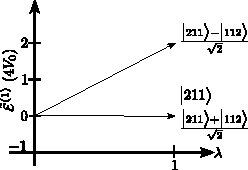
\includegraphics[width=0.4\textwidth]{EN02.pdf}
\end{figure}
\subsection*{Example}
\[
  \tilde{H} = 
  \begin{pmatrix}
  1-\epsilon & 0 & 0\\
  0 & 1 & \epsilon\\
  0 & \epsilon & 2
\end{pmatrix}\quad \text{Hamiltonian in matrix form}
\]
For $\epsilon \ll 1$:
\[
  \tilde{H} = 
  \underbrace{\begin{pmatrix}
  1 & 0 & 0\\
  0 & 1 & 0\\
  0 & 0 & 2
\end{pmatrix}}_{\hat{H}_0} + \epsilon 
  \underbrace{\begin{pmatrix}
  1 & 0 & 0\\
  0 & 0 & 1\\
  0 & 1 & 0
\end{pmatrix}}_{\mathcal{W}}
\]

\[
  \mathcal{E}_1 = \mathcal{E}_2 = 1, \quad \mathcal{E}_3 = 2
\]
\[
  \Rightarrow \big|\Psi_1\big> + \big|\Psi_2\big> \quad \text{are degenerate}
\]
But $ \big|\Psi_1\big> + \big|\Psi_2\big> $ are linearly independent in the perturbation.\\
We can use \emph{TINDPT} (non-degenerate for $\big|\Psi_1\big> \& \big|\Psi_2\big>$)
\begin{align*}
  \tilde{\mathcal{E}}_1 &= 1 + 
  \cancelto{\epsilon}{\big<\Psi_1\big|\hat{V}'\big|\Psi_1 \big>} + \sum_{n\neq 1}
  \frac{\big<\Psi_{n'}\big|\hat{V}'\big|\Psi_1 \big>}{\mathcal{E}_1 - 
  \mathcal{E}_{n'}} = 1-\epsilon\\
  \tilde{\mathcal{E}}_2 &= 1 + \cancelto{0}{\big<\Psi_2\big|\hat{V}'\big|\Psi_2 \big>} + \sum_{n\neq 2}
  \frac{\big<\Psi_{n'}\big|\hat{V}'\big|\Psi_2 \big>}{\mathcal{E}_2 - 
  \mathcal{E}_{n'}} = 1-\epsilon^2\\
  \tilde{\mathcal{E}}_3 &= 2 +\cancelto{0}{\big<\Psi_3\big|\hat{V}'\big|\Psi_3 \big>} +
  \frac{\epsilon^2}{2-1} = 2 + \epsilon^2
\end{align*}
\begin{figure}[H]
  \centering
	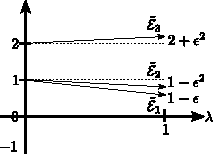
\includegraphics[width=0.4\textwidth]{EN4.pdf}
\end{figure}
\[
  \det 
  \begin{pmatrix}
  1-\omega & 0 & 0\\
  0 & 1-\omega & \epsilon\\
  0 & \epsilon & 2-\omega
\end{pmatrix}
 = 0 
\]
\begin{align*}
  \omega = 1 -\epsilon \quad (1 - \omega)(2-\omega) - \epsilon^2 &= 0\\
  \omega^2 - 3\omega + 2 - \epsilon^2 &= 0
\end{align*}
\[
  \boxed{\omega_\pm = \frac{3}{2} \pm \sqrt{\frac{9}{4}-2+\epsilon^2} = \frac{3}{2} \pm
  \sqrt{\frac{1}{4} + \epsilon^3}}
\]
\newpage
%%%%%%%%%%%%%%%%%%%%%%%%%%%%%%%%%%%%%%%%%%%%%%%%%%%%%%%%%%%%%%%%%%%%%%%%%%%%%%%%%%%%%%%%%%%%%%%%
%%%%%%%%%%%%%%%%%%%%%%%%%%%%%%%%%%%%%%%%%%%%%%%%%%%%%%%%%%%%%%%%%%%%%%%%%%%%%%%%%%%%%%%%%%%%%%%%
%%%%%%%%%%%%%%%%%%%%%%%%%%%%%%%%%%%%%%%%%%%%%%%%%%%%%%%%%%%%%%%%%%%%%%%%%%%%%%%%%%%%%%%%%%%%%%%%
\chapter{Fine Structure of the Hydrogen}
\section{Lecture 13}
May 23, 2023\\
\begin{wrapfigure}{l}{6cm}
  \begin{center}
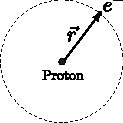
\includegraphics[width=0.2\textwidth]{FSTR.pdf}
\caption{Boohr model of the Hydrogen atom.}
  \end{center}
\end{wrapfigure}
\textbf{Hamiltonian}
\[
  \hat{H}_{0,\text{Bohr}} = \frac{-\hbar^2}{2m}\nabla^2_{\vec{r}}
  - \frac{e^2}{4\pi\epsilon_0}\frac{1}{r}=
  \boxed{\frac{\vec{\nabla}_{\vec{r}}}{2} - \frac{1}{r^2}}\quad
  \fbox{%
  \parbox{.15\textwidth}{%
  In atomic units}%
} 
\]
\textbf{Atomic units}
\[
  \hbar = m_e = e = 4\pi \epsilon_0 = 1 = a_0
\]
\textbf{but why?}
\subsection{Fine Structure Constant}
\[
  \alpha = \frac{e^2}{4\pi \epsilon_0 \hbar c} \cong \frac{1}{137,036}\quad
    \fbox{%
  \parbox{.2\textwidth}{%
  A universal dimensionless constant relating $4\pi\epsilon_0, e^2, \hbar\,\&\, c.$}%
}
\]
\[
  \Rightarrow c = \frac{1}{\alpha} \approx 137\quad \text{in atomic units.} 
\]
$\hat{H}_\text{Bohr}$ is the Bohr model for the hamiltonian of the hydrogen atom.\\
\\
\textbf{Idea:} Find corrections to the Bohr model hamiltonian $\hat{H}_\text{Bohr}$, and include
them via \emph{TIPT}.
\[
  \hat{H}_\text{Bohr} + \underbrace{\hat{H}'}_\text{corrections} \longrightarrow 
  \tilde{E}_n \approx E_n + \big<\varphi_n\big|\hat{H}'\big|\varphi_n\big>
\]
In fact, $\big<\varphi_n\big|\hat{H}'\big|\varphi_n\big>$ are of order $\alpha^4 m c^2$, whereas: 
\begin{align*}
  E_n &= \frac{E_1}{n^2} = \frac{-m_e e^4}{2(4\pi\epsilon_0)^2\hbar^2}\left(\frac{1}{n^2}\right)\\
      &= \frac{-m_e}{2}\underbrace{\left(\frac{e^2}{4\pi\epsilon_0 \hbar c}\right)^2}_\alpha
      \cdot c^2 \frac{1}{n^2}\\
      &= \frac{-m_e c^2}{2} \alpha^2 \frac{1}{n^2} = \mathcal{O}(mc^2\alpha^2)
\end{align*}
\[
  \hat{H}_\text{Bohr} (r) \longleftarrow \parbox{0.13\textwidth}{Angular symmetry}
  \Longrightarrow \varphi_{nlm}(r, \theta, \varphi)\zeta_n (r)Y_l^m (\theta,\varphi) 
\]
are $l$ and $m$ degenerate. So $\hat{H}'$ could split/ break this angular degeneracy.\\
\\
\textbf{Fine Structure $\mathcal{O}(\alpha^2 m_e c^2)$}
\begin{enumerate}
  \item Relativistic corrections to the Kinetic Energy.
  \item Spin-Orbit Coupling: this interaction between the electron's spin and its orbit around the 
    proton.\\
    $ \hat{H}_{SO} = -\vec{\mu}\cdot \vec{B}$
    \begin{itemize}
    \item $\vec{\mu}$ electron's spin dipole proton orbit induced.
    \item $\vec{B}$ magnetic field.
    \end{itemize}
\end{enumerate}
\[
  \hat{T}_\text{Bohr} = \frac{1}{2}(m\hat{p})^2, \quad \hat{p} = i \hbar \nabla_r
\]
\subsection{Relativistic corrections to the Kinetic Energy}
\textbf{Relativistic effects}
\[
  \text{Total Energy} = \text{Kinetic E} + \text{Rest E}
\]
\[E_0 = mc^2, \quad \gamma = \frac{1}{\sqrt{1 - v^2/c^2}}, \quad \hat{p} = \gamma mv\]
\[
  \parbox{0.08\textwidth}{Total Energy} = \gamma E_0 = \frac{mc^2}{\sqrt{1-v^2/c^2}}
\]
\[
  \parbox{0.08\textwidth}{Kinetic Energy} = \parbox{0.08\textwidth}{Total Energy} - 
  \parbox{0.08\textwidth}{Rest Energy} = \frac{mc^2}{\sqrt{1 -v^2/c^2}} - mc^2
\]
\begin{align*}
  \left(\parbox{0.08\textwidth}{Total Energy}\right)^2 &= \left(\frac{m^2c^4}{1-v^2/c^2}\right), 
  \quad p^2 = \frac{m^2v^2}{1-v^2/c^2}\\
  &= \left(\frac{m^2v^2c^2 + m^2 c^4 - m^2 v^4}{1-v^2/c^2}\right)\\
  &= p^2 c^2 + \frac{m^2 c^4 (1-v^2/c^2)}{1-v^2/c^2}\\
  &= p^2 c^2 + m^2 c^4
\end{align*}
\textbf{Steps}
\begin{enumerate}
  \item Square $E_\text{tot} = \gamma E_0$ so as to avoid the root.
  \item Separate out $p=\gamma m v$ by substracting $\gamma^2 m^2 v^2 c^2$.
  \item Express in terms of $p$ alone to avoid $v$ because it is not a good quantum operator.
\end{enumerate}
\[
 \left(\parbox{0.08\textwidth}{Total Energy}\right)^2 = \left(T + E_0 \right)^2 = 
 \left(T + mc^2\right)^2 = p^2 c^2 + m^2 c^4
\]
An expression relating $T$ to $p$ including relativistic effects but without $\gamma$ \& $v$.
\begin{align*}
  \Rightarrow \hat{T} &= \sqrt{p^2c^2 + m^2c^4} - mc^2, \quad \sqrt{1+x^2} \approx 
  1 + \frac{x^2}{2}-\frac{x^4}{8} + \mathcal{O}(x^6)\\
  &= mc^2 \left(\sqrt{1 +\frac{p^2}{mc^2}} - 1\right)\\
  &= mc^2 \left(1+\frac{p^2}{2m^2c^2} - \frac{p^4}{8m^4c^4} + \mathcal{O}\left(\frac{p^6}
  {m^6c^6}\right) - 1\right)\\
  &= \underbrace{\frac{p^2}{2m}}_\text{classic K.E} - 
  \underbrace{\frac{p^4}{8m(mc)^2}}_{\scriptsize \parbox{0.1\textwidth}{1st order relativistic correction}}
  + \mathcal{O}\left(\frac{p^6}{m^5c^4}\right)
\end{align*}
\begin{align*}
  \hat{H}_\text{rel} &= \frac{-p^4}{8m^3c^2} \quad\quad \parbox{0.5\textwidth}{The reletivistic 
  correction to the Bohr model hamiltonian. This hamiltonian is dependent only on $(p^2)^2$ 
and so has the same eigenvalues as the unperturbed Bohr hamiltonian.}\\
\\
    E^{(1)}_\text{rel} &= \bigg<\varphi_n \bigg|\frac{-p^4}{8m^3c^2}\bigg|\varphi_n\bigg>
\end{align*}
There is no angular dependence, so it does not lift the degeneracy between $\varphi_{nlm}$, and
we can use non-degenerate perturbation theory.
\[
  \Rightarrow \mathlarger{\varphi}_{nlm}\quad\text{are eigenstates of}\,\hat{H}_\text{rel}
\]
We can use non-degenerate perturbation theory.\\
\\
Treat $\hat{p}^2$ as an hermitian operator:
\[
  p^2 = \hbar^2 \nabla^2
\]
\[
  E_n^{(1)} = \frac{-1}{8m^3c^2} \big<\varphi_n\big|(\hat{p}^2)^\dagger(\hat{p}^2) \big|\varphi_n
  \big>
\]
From the Bohr Model
\[
  E_\text{tot} = T + V
\]
\[
  \Rightarrow p^2 = 2m(E_\text{tot} - \hat{V})
\]
this is a further approximation, but is justified as we are calculating $\big< 
\hat{H}_\text{rel}\big>$ perturbately.
\[
  E_n^{(1)} = \frac{-1}{8m^3c^2} \big<\varphi_n\big|2m(E_\text{tot} - \hat{V}^\dagger)2m
  (E_\text{tot} - \hat{V})\big|\varphi_n\big>
\]
But $E_\text{tot} = E_n$ when operating on $\varphi_n$
\begin{align*}
  &= \frac{-1}{2mc^2}\big<\varphi_n \big|(E_\text{tot} - \hat{V}^\dagger)
  (E_\text{tot} - \hat{V})\varphi_n\big>\\
  &= \frac{-1}{2mc^2}\left(E_n^2 - 2E_n\big<\varphi_n\big|\hat{V}\big|\varphi_n\big> + 
  \big|\big<\varphi_n\big|\hat{V}\big|\varphi_n \big>\big|^2\right)
\end{align*}
let $\big<\hat{V}\big> = \big<\varphi_n\big|\hat{V}\big|\varphi_n\big>$:
\[
 \frac{-1}{2mc^2}\left(E_n^2 - 2E_n\big<\hat{V}\big> + 
 \big|\big<\hat{V}\big>\big|^2\right) 
\]
$\hat{V} = \frac{-e^2}{4\pi\epsilon_0} \frac{1}{r}$:
\[
  \tilde{E}^{(1)}_{\text{rel},n} = \frac{-1}{2mc^2}\left(E_n^2 - 2E_n
      \left(\frac{-e^2}{4\pi\epsilon_0}\right)\bigg<\frac{1}{r}\bigg> + 
   \left(\frac{-e^2}{4\pi\epsilon_0}\right)^2\bigg<\frac{1}{r^2}\bigg>\right)
\]
\begin{align*}
  E_n &= \underbrace{\frac{-me^4}{2(4\pi\epsilon_0)^2}\frac{1}{\hbar^2}}_{E_1} \left(\frac{1}{n^2}
  \right) = \frac{-m}{2}\left(\frac{-e^2}{4\pi\epsilon_0}\right)^2\frac{1}{\hbar^2}\frac{1}{n^2}\\
    a_0 &= \frac{4\pi\epsilon_0\hbar^2}{me^2}, \quad E_1 = -\left(\frac{e^2}{4\pi\epsilon_0}\right)^2
    \frac{m}{2\hbar^2}\rightarrow \parbox{0.2\textwidth}{Negative, since the Bohr model hydrogen 
    atom is stable.}
\end{align*}
Then:
\begin{align*}
  \tilde{E}^{(1)}_{\text{rel},n} &= \frac{-1}{2mc^2} \left[\frac{E_1^2}{n^4} - 2\frac{E_1}{n^2}
      \left(\frac{-e^2}{4\pi\epsilon_0}\right)\bigg<\frac{a_0}{r}\bigg>\left(\frac{e^2m}
      {4\pi\epsilon_0\hbar^2}\right) + 
  \left(\frac{-e^2}{4\pi\epsilon_0}\right)^2\bigg<\frac{a_0^2}{r^2}\bigg>\left(\frac{e^2m}
{4\pi\epsilon_0\hbar^2}\right)^2 \right]\\
&=\boxed{ \frac{-E_1^2}{2mc^2}\left[\frac{1}{n^4}-\frac{4}{n^2}\bigg<\frac{a_0}{r}\bigg>+
4\bigg<\frac{a_0^2}{r^2}\bigg>\right]}
\end{align*}
We know that: (\emph{This results were taken from Griffits})
\begin{align*}
  \bigg<\varphi_n\bigg|\frac{1}{r}\bigg|\varphi_n\bigg> &= \frac{1}{n^2 a_0}\\
  \bigg<\varphi_n\bigg|\frac{1}{r^2}\bigg|\varphi_n\bigg> &= \frac{1}{(l+1/2)n^3 a_0^2}
\end{align*}
so,
\begin{align*}
  \tilde{E}^{(1)}_{\text{rel},n} &= \frac{-E_1^2}{2mc^2}\left[\frac{1}{n^4}
  -\frac{4}{n^4}+\frac{4}{(l+1/2) n^3}\right]\quad \parbox{0.15\textwidth}{factor out $\frac{1}
{n^4}$ to get $E_n^2$}\\
    &=\frac{-E_n^2}{2mc^2}\left[1-4+\frac{4n}
    {(l+1/2)}\right]\\
\Aboxed{\tilde{E}^{(1)}_{\text{rel},n} &=\frac{-E_n^2}{2mc^2}\left[\frac{4n}
    {(l+1/2)}-3\right]}
\end{align*}
%%%%%%%%%%%%%%%%%%%%%%%%%%%%%%%%%%%%%%%%%%%%%%%%%%%%%%%%%%%%%%%%%%%%%%%%%%%%%%%%%%%%%%%%%%%%%%
%%%%%%%%%%%%%%%%%%%%%%%%%%%%%%%%%%%%%%%%%%%%%%%%%%%%%%%%%%%%%%%%%%%%%%%%%%%%%%%%%%%%%%%%%%%%%%
%%%%%%%%%%%%%%%%%%%%%%%%%%%%%%%%%%%%%%%%%%%%%%%%%%%%%%%%%%%%%%%%%%%%%%%%%%%%%%%%%%%%%%%%%%%%%%
\newpage
\section{Lecture 14}
May 24, 2023
\begin{equation}
  \boxed{\tilde{E}^{(1)}_{\text{rel}} =\frac{-E_n^2}{2mc^2}\left[\frac{4n}
  {(l+1/2)}-3\right]}
  \end{equation}
So, $\big|\varphi_{nlm}\big>$ are eigenfunctions of $\hat{H}_\text{rel}$ and non-degenerate 
perturbation theory is valid.
\subsection{Spin-Orbit}
\[
  \hat{\tilde{H}}_{SO} = -\vec{\mu}\cdot \vec{B}_\text{ind}, \quad \text{where:}
\]
\begin{itemize}
  \item $\vec{\mu}$ is the electric spin dipole of the electron.
  \item $\vec{B}_\text{ind}$ is the magnetic field induced by the proton orbit.
\end{itemize}
\textbf{From the electron's perspective}

\begin{wrapfigure}[4]{l}{7cm}
  \begin{center}
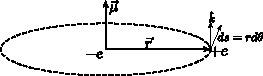
\includegraphics[width=0.4\textwidth]{SPO.pdf}
\caption{Hydrogen atom from the electron's perspective.}
  \end{center}
\end{wrapfigure}

\[
  \vec{B}_\text{ind} = \frac{\mu_0 I}{2r}, \quad \text{Biot-Savart law}
\]

\begin{align*}
  \vec{B}_\text{ind} &= \mu_0\int \frac{\vec{r}\times 
  d\vec{l}}{r^3}I, \quad d\vec{l}  = r\vec{e}_\theta d\theta\\
 &= \frac{\mu_0}{r^3}r^2\int_{0}^{2\pi} \frac{\hat{e}_r \times 
\hat{e}_\theta}{4\pi}d\theta I\\
 &= \frac{\mu_0 I}{2r}\hat{k}
\end{align*}
\textbf{Idea:} We'd prefer to have the hamiltonian in terms of "good" quantum operators of 
$\hat{H}_\text{Bohr}$, i.e. operators which have $\big|nlm\big>$ as eigenstates.\\
\\
\textbf{Why?} So we can use non-degenerate perturbation theory.\\
Can we express the current I in terms of a quantum operator with $\big|nlm\big>$ as 
eigenstates?\\
\\
Current is the speed of the proton as it orbits around the electron.\\
\\
Try to express I in terms of the electron-proton system's angular momentum L.
\[
  current = \frac{charge}{orobit\,\,period}\quad \text{assuming quasi-circular orbit}
\]
\[
  I = \frac{e}{T}
\]
\[
  \parbox{0.25\textwidth}{angular momentum of the electron around proton}  =
  r m_e v
\]
\[
  r m_e v = r m_e \frac{2\pi r}{T}
\]
\begin{align*}
  \vec{B}_\text{ind} &= \frac{\mu_0}{2r}\left(\frac{e}{T}\right)\cdot\hat{k}\\
&= \frac{\mu_0 e}{2r} \frac{1}{2\pi m_e r^2}\underbrace{\left(\frac{2\pi m_e r^2}{T}\right)}
_{L}\hat{k}
\end{align*}
\begin{align*}
  \vec{B}_\text{ind} &= \frac{\mu_0 e}{4\pi m_e r^3}\vec{L}, \quad c^2 = 
  \frac{1}{\mu_0 \epsilon_0}, \quad \mu_0 = \frac{1}{\epsilon_0 c^2}\\
                     &= \frac{e}{4\pi \epsilon_0 r^3}\frac{\vec{L}}{m_e c^2} 
\end{align*}
Can we express $\vec{\mu}$ in terms of a "good" quantum operator for $\hat{H}_\text{Bohr}$?\\
\\
The magnetic dipole momentum of the electron considers the electron to be a "ring" 
of charge of radius r with units of charge q distributed over the string.
\begin{figure}[H]
  \centering
	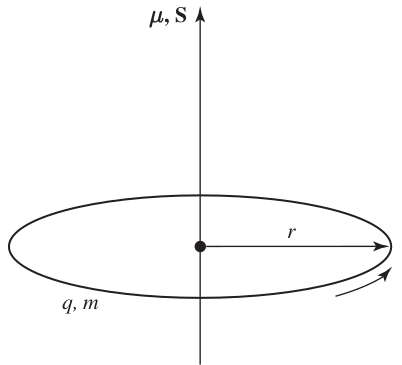
\includegraphics[width=0.4\textwidth]{RNG.png}
  \caption{A ring of charge, rotating aorund the axis.}
\end{figure}
$$
v = \frac{2\pi r}{T}
$$
\begin{align*}
  \big|\vec{\mu}\big| &= I\cdot A \longrightarrow \text{current}\times\text{area}\\
                      &= \frac{q}{T} \times \pi r^2
\end{align*}
Can we relate $\vec{\mu}$ to the electron spin operator $\vec{S}$.
\begin{align*}
  \parbox{0.2\textwidth}{angular momentum of a spinning ring} 
  \quad &= \quad \parbox{0.1\textwidth}{moment of inertia} \quad \times \quad
  \parbox{0.1\textwidth}{angular velocity}\\
        &= m\,r^2 \times \frac{2\pi}{T}
\end{align*}
\[
  S  = \frac{2\pi r^2m_e}{T}
\]
\[
  \vec{S} = \frac{2\pi r^2 m_e \vec{k}}{T}
\]
\[
  \vec{\mu} = \frac{q \pi r^2}{T}\vec{k} = \frac{q\vec{S}}{2m_e}
\]
\[
  \left.\begin{aligned}
        \vec{\mu}_e = \frac{-e\vec{S}}{2m_e}
       \end{aligned}
 \right\}
 \qquad \text{classical result}
\]
Using Dirac's relativistic quantum mechanics we obtain an extra factor of 2, so that:
\[
  \left.
  \vec{\mu}_e = \frac{e \vec{S}}{m_e}
\right\} \quad
\parbox{0.2\textwidth}{quantum mechanical result for an electron}
\qquad \left(\parbox{0.1\textwidth}{Dirac Eqn} \right)
\]
However, we treated the proton's motion around the electron as if the electron was in an inertial
frame of reference.
This in not the case as the electron has an acceleration.
\[
  \vec{B}_\text{ind} = \frac{e \vec{L}}{4\pi \epsilon_0 r^3 m_e c^2}
\]
To account for this, we need to include the Thomas Precession correction, a factor of $1/2$ in
$\vec{B}_\text{ind}$.
\[
  \left.
  \vec{B}_\text{ind} = \frac{e\vec{L}}{8\pi \epsilon_0 r^3 m_e c^2}
\right\}
\qquad \parbox{0.1\textwidth}{including relativistic effects}
\qquad \left(\parbox{0.1\textwidth}{Thomas Precession} \right)
\]
In any case: 
\[
  \hat{\tilde{H}}_{SO} = -\vec{\mu}\cdot \vec{B}_\text{ind}
\]
Negative ensures $\big<\hat{H}_{SO} \big>$ is positive when $\vec{\mu}$ and $\vec{B}$ are 
parallel.\\
\\
Substituting in: 
\begin{align*}
  \hat{\tilde{H}}_{SO} &= -\left(\frac{e\vec{S}}{m_e} \right)\left(\frac{e\vec{L}}
  {8\pi\epsilon_0 r^3 m_e c^2} \right)\\
                       &= \frac{e^2}{8\pi \epsilon_0 r^3}\frac{\vec{S}\vec{L}}{m_e m_p c^2}
\end{align*}
Since $\big|\varphi_{nlm} \big>$ have $S$ and $L$ as quantum numbers, $\vec{S}$ and $\vec{L}$
 have $\big|nlm \big>$ as eigenstates, and we can use non-degenerate perturbation theory.
 \begin{align*}
   \tilde{E}^{(1)}_{SO} &= \bigg<\varphi_{nlm}\bigg| \frac{e^2 \vec{S}\cdot\vec{L}}
   {8\pi \epsilon_0 m_e m_p c^2 r^3}\bigg|\varphi_{nlm}\bigg>\\
                        &= \frac{e^2}{8\pi\epsilon_0 m_e m_p c^2}
                        \bigg< \frac{\vec{S}\cdot\vec{L}}{r^3}\bigg>
 \end{align*}
 but $\vec{S}$ and $\vec{L}$ commute with $r$:
 \[
 \tilde{E}^{(1)}_{SO}=\frac{e^2}{8\pi\epsilon_0 m_e m_p c^2}
\bigg<\vec{S}\cdot\vec{L}\bigg>\bigg<\frac{1}{r^3}\bigg>
 \]
\begin{align*}
  \big<L^2\big>  &= \hbar^2\, l(l + 1)\\
  \big<S^2\big> &= \hbar^2\, s(s+1)\\
  \big< J^2\big> &= \hbar^2\,j(j+1)
\end{align*}
\[
  \vec{J} = \vec{S} + \vec{L}
\]
\[
  J^2 =\left(\vec{S} + \vec{L}\right)^2 = S^2 + 2\,\vec{S}\cdot \vec{L} + L^2 
\]
\[
  \Rightarrow \vec{S}\cdot\vec{L} = \frac{1}{2}\left(J^2 - S^2 - L^2\right)
\]
\begin{align*}
  \big<\vec{S}\cdot \vec{L} \big> &= \frac{\big<J^2\big> - \big<S^2\big> - \big<L^2\big>}
  {2}\\
  &= \frac{\hbar^2}{2}\left(j(j+1) - s(s+1)- l(l+1)\right)
\end{align*}
\[
  \bigg< \frac{a_0^3}{r^3}\bigg> = \frac{1}{l(l+1/2)(l+1)n^3}
\]
\[
  \tilde{E}^{(1)}_{SO} = \frac{e^2}{2(4\pi\epsilon_0)m_e m_p c^2 a_0^3}\frac{\hbar^2}{2}
  \frac{j(j+1) - s(s+1)- l(l+1)}{l(l+1/2)(l+1)n^3}
\]
\[
  E_n = \frac{-m_e e^4}{2(4\pi\epsilon_0)^2\hbar^2}\frac{1}{n^2}
\]
\[
  a_0 = \frac{4\pi \epsilon_0 \hbar^2}{m_e e^2}
\]
\begin{align*}
  \tilde{E}^{(1)}_{SO} &= \frac{e^2}{4(4\pi\epsilon_0)m_e m_p c^2}\left(\frac{m_e e^2}
  {4\pi\epsilon_0\hbar^2}\right)^3
 \hbar^2\frac{j(j+1) - s(s+1)- l(l+1)}{l(l+1/2)(l+1)n^3}\\
  &= \underbrace{\left(\frac{m_e e^4}{2(4\pi\epsilon_0)^2 \hbar^2}\right)^2 \frac{1}{n^4}}
  _{E_n^2}
  \frac{1}{mc^2}\frac{n[j(j+1) - s(s+1)- l(l+1) ]}{ l(l+1/2)(l+1) }
  \end{align*}
  \begin{equation}
    \boxed{
  \tilde{E}_{SO}^{(1)} = \frac{E_n^2}{mc^2} \frac{ n[j(j+1) - s(s+1)- l(l+1) ] }
  {l(l+1/2)(l+1)}
}
\end{equation}
The relativistic and spin-orbit corrections have the same "order":
\[
  \frac{E_n^2}{mc^2} = \frac{\alpha^4 mc^2}{n^4} = \frac{\alpha^2 E_n}{n^2}
\]
\textbf{Idea:} We must include both corrections or neither.
\newpage
\clearpage
\subsection{Fine Structure Correction}
\begin{align*}
  E_{fs} &= \tilde{E}^{(1)}_\text{rel} + \tilde{E}_{SO}^{(1)} = \frac{E_n^2}{mc^2}
  \left[\frac{-2n}{l+1/2} + \frac{3}{2} + \frac{ n[j(j+1) - s(s+1)- l(l+1) ] }
  {l(l+1/2)(l+1)} \right]\\
         &= \frac{E_n^2}{mc^2}\left[\frac{3}{2}+\frac{n}{l+1/2} \frac{ 
j(j+1) - s(s+1)- l(l+1) - 2l(l+1)
         }{l(l+1)} \right]\\
&= \frac{E_n^2}{mc^2}\left[ \frac{3}{2} + \frac{n}{l+1/2} 
\frac{ j(j+1) - s(s+1) - 3l(l+1)}{l(l+1)}\right]
\end{align*}
\textbf{Note:} $s =1/2$, $j = l \pm s = l \pm 1/2$, $\Rightarrow -s(s+1)=-1/2(3/2) = -3/4$ 
\[
  =\frac{E_n^2}{mc^2}\left[ \frac{3}{2} + \frac{n}{l+1/2} 
\frac{ j(j+1) - 3/4 - 3l(l+1)}{l(l+1)}\right] 
\]
if $j= l+s = l + 1/2$ (angular and spin angular momentum are parallel) $\Rightarrow 
l = j - 1/2, l+1= j+1/2, l+1/2= j$
\begin{align*}
  &=\frac{E_n^2}{mc^2}\left[ \frac{3}{2} + \frac{n}{j} 
\frac{ j(j+1) - 3/4 - 3(j-1/2)(l+1)}{(j-1/2)(l+1)}\right]  \\
  &=\frac{E_n^2}{mc^2}\left[ \frac{3}{2} + \frac{n}{j} 
\frac{ j^2+j - 3/4 - 3(j^2-1/4)}{j^2-1/4}\right]\\
  &= \frac{E_n^2}{mc^2}\left[\frac{3}{2}+ \frac{n[-2j+j]}{j(j^2-1/4)} \right]\\
  &= \frac{E_n^2}{mc^2}\left[\frac{3}{2}+\frac{2n\cancel{(j-1/2)}}
  {\cancel{(j-1/2)}(j+1/2)}\right]\\
  &= \frac{E_n^2}{2mc^2}\left[3-\frac{4n}{j+1/2}\right]
\end{align*}
if $j=l-s = l-1/2$, $l = j+1/2$, $l+1=j+3/2$, $l+1/2=j+1$ (l and s are anti-parallel)
\begin{align*}
  E_{fs} &= \frac{E_n^2}{mc^2}\left[\frac{3}{2} + \frac{n[j(j+1)-3/4 - 3(j+1/2)(j+3/2)]}
  {(j+1/2)(j+1)(j+3/2)}\right]\\
&= \frac{E_n^2}{mc^2}\left[\frac{3}{2}+\frac{n[j^2+j-3/4-3(j^2+2j+3/4)]}
   {(j+1/2)[j^2 +5/2 j +3/2]} \right]\\
&= \frac{E_n^2}{mc^2}\left[\frac{3}{2}+\frac{n\cancelto{2}{[-2j^2-5j-3]}}{(j+1/2)
\cancel{[j^2+5/2j+3/2]}} \right]\\
&= \frac{E_n^2}{mc^2}\left[\frac{3}{2}-\frac{2n}{j+1/2}\right]\\
&= \frac{E_n^2}{2mc^2}\left[3-\frac{4n}{j+1/2}\right]
\end{align*}
Finally
\begin{equation}
  \tilde{E} = E_n + \frac{E_n^2}{2mc^2}\left[3 - \frac{4n}{j+1/2}\right]
\end{equation}
\newpage
%%%%%%%%%%%%%%%%%%%%%%%%%%%%%%%%%%%%%%%%%%%%%%%%%%%%%%%%%%%%%%%%%%%%%%%%%%%%%%%%%%%%%%%%%%%%%%%%
%%%%%%%%%%%%%%%%%%%%%%%%%%%%%%%%%%%%%%%%%%%%%%%%%%%%%%%%%%%%%%%%%%%%%%%%%%%%%%%%%%%%%%%%%%%%%%%%
%%%%%%%%%%%%%%%%%%%%%%%%%%%%%%%%%%%%%%%%%%%%%%%%%%%%%%%%%%%%%%%%%%%%%%%%%%%%%%%%%%%%%%%%%%%%%%%%
%%%%%%%%%%%%%%%%%%%%%%%%%%%%%%%%%%%%%%%%%%%%%%%%%%%%%%%%%%%%%%%%%%%%%%%%%%%%%%%%%%%%%%%%%%%%%%%%
\section{Lecture 15}
May 29, 2023
\[
  \hat{H}_{Bohr} = \frac{-\hbar^2}{2m}\nabla^2 - \frac{e^2}{4\pi \epsilon_0}\frac{1}{r}
\]
\begin{align*}
  \hat{T} &= \underbrace{mc^2}_{E_0}\left(\sqrt{1 - \frac{p^2}{m^2c^2}}-1\right)\\
          &\approx \cancel{mc^2}\left(\frac{p^2}{2\cancel{m^2c^2}} - \frac{p^4}{8\cancel{
          m^4c^4}}+ \mathcal{O}\left(\frac{p^6}{m^6c^6}\right)\right)\\
          &= \underbrace{\frac{p^2}{2m}}_{\hat{T}} + 
          \underbrace{\frac{p^4}{8m^3c^2}}_{\hat{H}_{rel}} + \cdots
\end{align*}
Where $\hat{H}_{rel}$ is the first order relativistic correction to the kinetic energy.
\[
  E_{rel} = \tilde{\mathcal{E}}^{(1)}_{rel} = \frac{-1}{8m^3c^2}\left(
  \big<\psi_n\big|p^4\big|\psi_n \big>\right)
\]
Treating the momentum as a quantum operator we had: $\hat{p}=i\hbar\vec{\nabla}$ (a 
semiclassical approximation).
\[
  \frac{\hat{p}^2}{2m}\big|\psi_n\big> = \left(E_n - \hat{V} \right)\big|\psi_n\big> \qquad
  \left(\parbox{0.2\textwidth}{to first order in the relativistic correction}\right)
\]
\begin{align*}
  E_{rel} &= \big<\psi_n\big|\hat{p}^{2\dagger}\hat{p}^2\big|\psi_n \big>
  \left(\frac{-1}{8m^3c^2}\right)\\
  &= \frac{-1}{8m^3c^2}\big<\psi_n\big|(E_n - \hat{V}^\dagger)2m\cdot 2m(E_n-\hat{V})
  \big|\psi_n\big>\\
  &= \frac{-1}{2mc^2}\left(\big<\psi_n\big|E_n^2 - 2E_n\hat{V} + 
  \big|\hat{V}\big|^2\big|\psi_n\big>\right)
\end{align*}
\[
  E_{rel,n}^{(1)} = -\frac{E_n^2 - 2E_n\big<\hat{V}\big> + \big<\hat{V}^2\big>}{2mc^2}
\]
\subsection*{Example: Harmonic Oscillator}
\[
  \mathcal{E}_n = \hbar\omega\left(n - \frac{1}{2}\right), \qquad n \in \mathbb{N}, \qquad
  \omega^2 = \frac{k}{m}
\]
\[
  \hat{V}_{harm} = \frac{1}{2}kx^2 = \frac{\omega^2 m x^2}{2}
\]
\[
  x = \sqrt{\frac{\hbar}{2m\omega}}\left(\hat{a}_+ - \hat{a}_-\right)
\]
\textbf{Recall:}
\[
  \big<\hat{T}\big> + \big<\hat{V}\big> = E_{tot} \Rightarrow \big<\hat{V}\big> = 
  \frac{\hbar\omega}{2}\left(n - \frac{1}{2}\right)
\]
Virial Theorem:
\[
  \big<\hat{T}\big> = \big< \hat{V}\big> \Rightarrow \big<\hat{V}\big> = \frac{E_{tot}}{2}
\]
\begin{align*}
  \big<\hat{V}\big> &= \frac{\hbar^2}{4m^2\omega^2}\left(\hat{a}_+ - \hat{a}_-\right)^4
  \frac{\omega^4m^2}{4}\\
                    &= \left(\frac{\hbar\omega}{4}\right)^2 \left(\hat{a}_+ - \hat{a}_-\right)^4
\end{align*}
\[
  a_+|n\rangle=\sqrt{n+1}|n+1\rangle
\]
\[
a_-|n\rangle=\sqrt{n}|n-1\rangle 
\]
\begin{align*}
  \left(\hat{a}_{+} + \hat{a}_{-}\right)^4 &=\left(\hat{a}_{+}^2+\hat{a}_{+}\hat{a}_{-} 
    + \hat{a}_{-}
    \hat{a}_{+} + \hat{a}_{-}^2\right)\left(\hat{a}_{+}^2+\hat{a}_{+}\hat{a}_{-} 
    +\hat{a}_{-}\hat{a}_{+} + \hat{a}_{-}^2\right)\\
  &=\big(\hat{a}_{+}^4+\hat{a}_{+}^2\hat{a}_{+}\hat{a}_{-}+\hat{a}_{+}^2\hat{a}_{-}\hat{a}_{+} +
    \hat{a}_{+}^2\hat{a}_{-}^2+\hat{a}_{+}\hat{a}_{-}\hat{a}_{+}^2 + \hat{a}_{+}\hat{a}_{-}
    \hat{a}_{+}
    \hat{a}_{-} + \hat{a}_{+}\hat{a}_{-}\hat{a}_{-}\hat{a}_{+}\\
  &+\hat{a}_{+}\hat{a}_{-}\hat{a}_{-}^2 + \hat{a}_{-}\hat{a}_{+}\hat{a}_{+}^2 + 
  \hat{a}_{-}\hat{a}_{+}
  \hat{a}_{+}\hat{a}_{-} + \hat{a}_{-} \hat{a}_{+}\hat{a}_{-}\hat{a}_{+} 
  + \hat{a}_{-}\hat{a}_{+}\hat{a}_{-}^2\\
&+\hat{a}_{-}^2 \hat{a}_{+}^2 + \hat{a}_{-}^2\hat{a}_{+}\hat{a}_{-} + \hat{a}_{-}^2
\hat{a}_{-}\hat{a}_{+} + \hat{a}_{-}^2\hat{a}_{-}^2\big)
\end{align*}
\begin{align*}
  \big<n\big|\left(\hat{a}_{+} + \hat{a}_{-}\right)^2\big|n\big> &=
 \big<n\big|\hat{a}_{+}^4\big|n\big> + \big<n\big| \hat{a}_+^2\hat{a}_{+}\hat{a}_{-}
\big|n\big> + \big<n\big|\hat{a}{+}^2\hat{a}_{-}\hat{a}_{+}\big|n\big>\\
&+\big<n\big|\hat{a}_{+}^2\hat{a}_{-}^2\big|n\big> +\big<n\big|\hat{a}_{+}
\hat{a}_{-}\hat{a}_{+}^2\big> \\
&+\big<n\big|\hat{a}_{+}\hat{a}_{-}\hat{a}_{+}\hat{a}_{-}\big|n\big>
+ \big< n\big|\hat{a}_{+}\hat{a}_{-}\hat{a}_{-}\hat{a}_{+}\big|n\big> + \big<n\big|\hat{a}_{+}
\hat{a}_{-}\hat{a}_{-}^2\big|n\big>\\
&+\big< n\big|\hat{a}_{-}\hat{a}_{+}\hat{a}_{+}^2\big|n\big> + 
\big<n\big|\hat{a}_{-}\hat{a}_{+}\hat{a}_{+}\hat{a}_{-}\big|n\big> + 
\big<n\big|\hat{a}_{-}\hat{a}_{+}\hat{a}_{-}\hat{a}_{+}\big|n\big>\\
&+\big<n\big|\hat{a}_{-}\hat{a}_{+}\hat{a}_{-}^2\big|n\big> + 
\big<n\big|\hat{a}_{-}^2\hat{a}_{+}^2\big|n\big>
+\big<n\big|\hat{a}_{-}^2\hat{a}_{+}\hat{a}_{-}\big|n\big>\\
&+ \big<n\big|\hat{a}_{-}^2\hat{a}_{-}\hat{a}_{+}\big|n\big> +
\big<n\big|\hat{a}_{-}^4\big|n\big>
\end{align*}
\begin{align*}
  &=n(n-1)+n^2+n(n+1)+n(n+1)+(n+1)^2+(n+2)(n+1) \\
  &=n^2-n+n^2+2 n^2+2 n+n^2+2 n+1+n^2+3 n+2 \\
  &=6 n^2+6 n+3=6\left(n^2+n+1 / 2\right)
\end{align*}
\[
  \big<\hat{V}^2\big> = \frac{3}{8}\hbar^2\omega^2\left(n^2+n+\frac{1}{2}\right),
  \qquad E_n^2 = \hbar^2\omega^2 \left(n-\frac{1}{2}\right)^2= 
  \hbar^2 \omega^2\left(n^2 - n + \frac{1}{4}\right)
\]
\[
  -2E_n\big<\hat{V}\big> = -2E_n \frac{E_n}{2} = -E_n^2, \qquad \text{recall:}\quad \big<n\big
  |\hat{V}\big|n\big> = \frac{E_n}{2}
\]
\begin{align*}
  E_{rel} &= \frac{1}{2mc^2}\left(E_n^2 - 2E_n\frac{E_n}{2}+ \frac{3}{8}\hbar^2\omega^2 
  \left(n^2+n+\frac{1}{2}\right)\right)\\
          &= \frac{3\hbar^2\omega^2}{16mc^2}\left(n^2+n+\frac{1}{2}\right), 
          \qquad \omega^2 = \frac{k}{m},\qquad E_1 = \frac{\hbar\omega}{2}\\
          &= \frac{3E_1^2}{4mc^2}\left(n^2+n+\frac{1}{2}\right), \qquad 
          E_{tot} = E_1 \left[(2n-1)+\frac{3E_1}{4mc^2}\left(n^2+n+\frac{1}{2}\right)\right],
          \qquad \frac{E_1}{mc^2}\ll 1
  \end{align*}
\[
  E_1 = \frac{\hbar\omega}{2} = \frac{\hbar}{2}\sqrt{\frac{k}{m}} \Rightarrow 
  \frac{\hbar\omega}{2} = \sqrt{\frac{k}{m}}\ll mc^2
\]
Then:
\[
  \tilde{\mathcal{E}}^{(1)}_{rel} = \frac{1}{2mc^2}\left( E_n^2 - 2E_n\bigg<
  nlm \bigg|\frac{-e^2}{4\pi\epsilon_0 r} \bigg|nlm\bigg> + \bigg<nlm\bigg|\frac{e^4}
{(4\pi\epsilon_0)^2r^2}\bigg|nlm\bigg>\right)
\]
\[
  E_1 = \frac{-me^4}{2(4\pi\epsilon_0)^2\hbar^2}, \qquad a_0 = \frac{4\pi\epsilon_0\hbar}{m_ee^2},
  \qquad \text{(for the Bohr atom)}
\]
\[
  \tilde{\mathcal{E}}^{(1)}_{rel} = \frac{-E_1^2}{2mc^2} \left(\frac{1}{n^4}- \frac{4}{n^2}
  \bigg<\frac{a_0}{r}\bigg> + 4 \bigg<\frac{a_0^2}{r^2}\bigg>\right)
\]
\begin{align*}
  \bigg<nlm\bigg|\frac{1}{r}\bigg|nlm\bigg> &= \frac{1}{n^2a_0} \\
  \bigg<nlm\bigg|\frac{1}{r^2}\bigg|nlm\bigg> &= \frac{1}{(l+1/2)n^3a_0^2}
\end{align*}
\[
  \boxed{\tilde{\mathcal{E}}^{(1)}_{rel, n} = \frac{-E_n^2}{2mc^2}\left(\frac{4n}{l+1/2}-3\right)}
\]
\[
  E_1 = \frac{\alpha^2mc^2}{2} = 13.8\,eV = -Rdy = \frac{-Ha}{2}
\]
\subsection{Spin-Orbit Coupling}
\[
  \boxed{\hat{H}_{SO} = -\vec{\mu}\cdot \vec{B}_{ind}}
\]
\begin{align*}
  \vec{\mu} &= \frac{-e\vec{S}}{m}\\
  \vec{B}_{ind} &= \frac{e\vec{L}}{8\pi\epsilon_0 mc^2 r^3}
\end{align*}
then:
\[
  \hat{H}_{SO} = \frac{e^2\,\vec{S}\cdot\vec{L}}{8\pi\epsilon_0 m^2c^2r^3}
\]
\begin{align*}
  \big<nlm\big|S^2\big|nlm\big> &= \hbar^2\,s(s+1) = \frac{3}{4}\hbar^2\\
 \big<nlm\big|L^2\big|nlm\big> &= \hbar^2\,l(l+1)
\end{align*}
Let $\vec{J} = \vec{L}+\vec{S}$, be the total angular momentum.
\[
   \big<nlm\big|J^2\big|nlm\big> = \hbar^2\,j(j+1)
\]
\textbf{Note:}
\[
  J^2 = \left(\vec{L}+\vec{S}\right)^2 = L^2 + S^2 + 2\,\vec{L}\cdot\vec{S}
\]
\[
  \Rightarrow \vec{S}\cdot\vec{L} = \frac{1}{2}\left(J^2 -L^2 -S^2 \right)
\]
\begin{align*}
  \big<nlm\big|\hat{H}_{SO}\big|nlm\big> &= \frac{e^2}{8\pi\epsilon_0m^2c^2}
  \bigg<\frac{\vec{S}\cdot\vec{L}}{r^3}\bigg>\\
&=\frac{e^2}{16\pi\epsilon_0m^2c^2}\bigg< \frac{J^2-L^2-S^2}{r^3}\bigg>\\
&=\frac{e^2}{16\pi\epsilon_0m^2c^2}\left(\big<J^2\big> - \big<L^2\big>-\big<S^2\big>\right)
\bigg< \frac{1}{r^3}\bigg>\\
&=\frac{e^2\hbar^2}{16\pi\epsilon_0m^2c^2}\cdot\frac{j(j+1)-s(s+1)-l(l+1)}{l(l+1/2)(l+1)n^3a_0^3},
\qquad \frac{1}{a_0^3}= \left(\frac{m_ee^2}{4\pi\epsilon_0\hbar^2}\right)^3\\
&= \underbrace{\frac{1}{4}\left(\frac{e^4}{(4\pi\epsilon_0)^2}\right)^2\cdot\frac{m^2}{\hbar^4}}
_{E_1^2}\frac{1}{mc^2}\left(\frac{1}{n^4}\right)\cdot
\frac{n[j(j+1)-s(s+1)-l(l+1)]}{l(l+1/2)(l+1)}
\end{align*}
\begin{align*}
  E_{SO} &= \frac{E_n^2}{mc^2}\cdot\frac{n[j(j+1)-l(l+1)-3/4]}{l(l+1/2)(l+1)}\\
         &= \frac{\alpha^4 m c^2}{4n^4}\frac{n[j(j+1)-l(l+1)-3/4]}{l(l+1/2)(l+1)}
\end{align*}
\begin{align*}
  E_{fs} &= E_{rel} + E_{SO}\\
         &= \frac{E_n^2}{2mc^2}\left[3-\frac{4n}{j+1/2} \right]\\
         &= \frac{\alpha^4 mc^2}{8n^4}\left[3-\frac{4n}{j+1/2} \right]
\end{align*}
\begin{align*}
  E_{tot} &= E_n + E_{rel} +E_{SO}\\
          &= -\frac{\alpha^2mc^2}{2n^2}\left[1+\frac{\alpha^2}{n^2}\left[
          \frac{n}{j+1/2}-\frac{3}{4}\right]\right]
\end{align*}
\[
  E_{fs}\sim \frac{\alpha^2}{n^2} \sim \frac{1}{10^6\cdot n^2}
\]
\[E_{fs} \sim \frac{1}{n}\]
The fine structure correction to $H$ is quite small, and most important for the ground state.
\newpage
%%%%%%%%%%%%%%%%%%%%%%%%%%%%%%%%%%%%%%%%%%%%%%%%%%%%%%%%%%%%%%%%%%%%%%%%%%%%%%%%%%%%%%%%%%%%%%%
%%%%%%%%%%%%%%%%%%%%%%%%%%%%%%%%%%%%%%%%%%%%%%%%%%%%%%%%%%%%%%%%%%%%%%%%%%%%%%%%%%%%%%%%%%%%%%%
%%%%%%%%%%%%%%%%%%%%%%%%%%%%%%%%%%%%%%%%%%%%%%%%%%%%%%%%%%%%%%%%%%%%%%%%%%%%%%%%%%%%%%%%%%%%%%%
\section{Lecture 16}
May 30, 2023
\[
  \tilde{E}_n = \frac{E_n}{2} \left[1 + \frac{\alpha^2}{n^2} \left(\frac{n}{j+1/2} -
  \frac{3}{4}\right)\right],\quad \text{where}\,\,\alpha^2=\left(\frac{1}{137.0}\right)^2
\approx 5.328\times 10^{-6}
\]
$\tilde{E}_1 = -13.605\,eV$\\
$E_{fs} \sim 0.725\,meV \sim 8.4\,K$\\
$k_BT \sim 25\,meV$ @ room temperature.\\
\\
Fine structure corrections are quite small, almost negligible, but definitely measurable @ 
liquid nitrogen temperatures $\sim 7-8\,K$. $E_{fs}$ is of the same order as these thermal
fluctuations.\\
\\
\textbf{Note:} $E_{fs} \approx \frac{E_1 \alpha^2}{n^4}\left(\frac{n}{j+1/2} - \frac{3}{4}
\right)$
\[
  E_{fs,n=1} \approx E_1\alpha^2\left(\frac{1}{1/2 + 1/2} - \frac{3}{4}\right) = 
  \frac{E_1 \alpha^2}{4}
\]
But for $n>1$, $E_{fs}$ lifts the degeneracy over angular momentum $l$, 
since $j = l+s = l\pm \frac{1}{2}$
\[
  l\ll  n-1, \qquad j = l \pm 1/2
\]
$l=1,\quad j=3/2$ or $1/2$
\begin{align*}
  E_{fs} &= \frac{E_1\alpha^2}{16}\left(\frac{2}{3/2+1/2} - \frac{3}{4}\right)\\
         &= \frac{E_1 \alpha^2}{16}\left(\frac{1}{4}\right)
\end{align*}
$n=3,\quad l=0$
\begin{align*}
  E_{fs} &= \frac{E_1\alpha^2}{81}\left(\frac{3}{1/2+1/2}-\frac{3}{4}\right)\\
         &= \frac{E_1 \alpha^2}{81}\left(\frac{9}{4}\right) = \frac{E_1\alpha^2}{36}
\end{align*}
$l=1, \quad s= -1/2, \quad j=1/2$
\[
  E_{fs} = E_{fs}(n=3, l=0)
\]
$l=1,\quad s = 1/2, j = 3/2$
\[
  E_{fs}= \frac{E_1\alpha^2}{81}\left(\frac{3}{3/2+1/2} -\frac{3}{4} \right) =
  \frac{E_1\alpha^2}{108}
\]
$l=2,\quad j=2\pm 1/2 = 5/2\,\,\,\text{or}\,\,\,3/2$\\
For $j=5/2$
\begin{align*}
  E_{fs}(3, j=5/2) &= \frac{E_1\alpha^2}{81}\left(\frac{3}{5/2+1/2}-\frac{3}{4}\right)\\
                   &= \frac{E_1\alpha^2}{324}
\end{align*}
\begin{figure}[H]
  \centering
  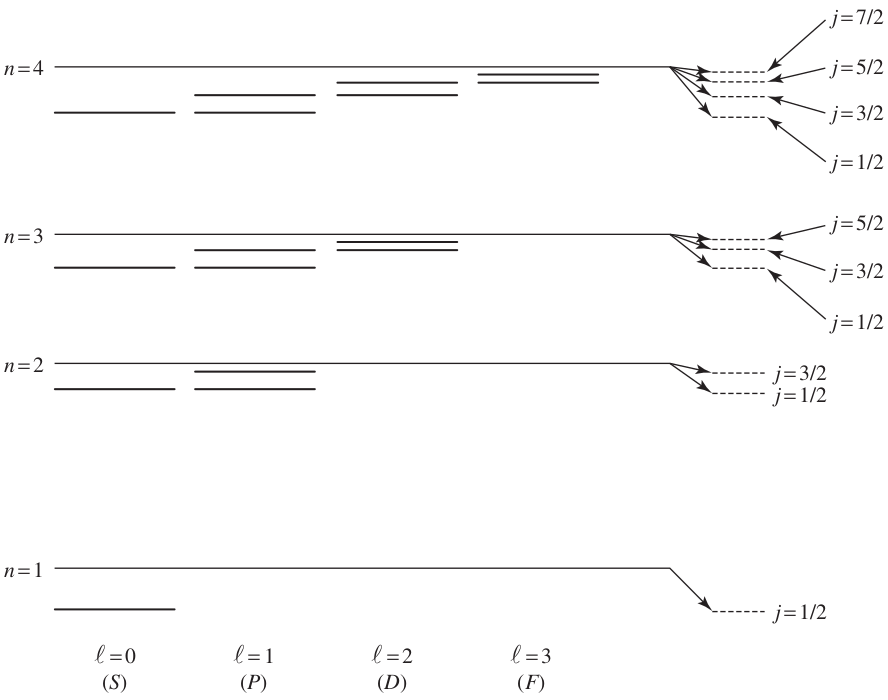
\includegraphics[width=0.8\textwidth]{FSE.png}
  \caption{Energy levels of hydrogen, including fine structure (\emph{Griffits})}
\end{figure}
\noindent
\textbf{Note:} splitting is over j in the energies. States with the same total angular momentum 
j are degenerate.
\begin{figure}[H]
  \centering
  \includegraphics[width=0.5\textwidth]{HEFS.pdf}
  \caption{Splitting of the energies over j, (not at scale).}
\end{figure}
\noindent
The "good" quantum numbers, i.e. the operators which commute with the states are 
$n, j, m_j, l,s \Longleftrightarrow  \vec{J},J_z, \vec{L}, \vec{S}$.
\[
\Rightarrow \big|n,j\big>, \quad m_l, \quad m_s , \quad (L_z, S_z)
\]
are no longer "good" quantum numbers/ operators.

\[
  \big|n,j\big> \longrightarrow \sum_{l,m_s,s,m_s} C_{n,j}\big|lm_l\big>\big|sm_s\big>\qquad
  \text{(Clebsk-London Coefficients)}
\]
\section{Exact solution via solving the Dirac's Eqn.}
\[
  \tilde{E}_{nj} = mc^2 \left[\left(1+\left(\frac{\alpha}{n-(j+1/2)+\sqrt{(j+1/2)^2-\alpha^2
  } }\right)^2\right)^{-1/2}+1\right]
\]
Expand to order $\alpha^4mc^2$:\\
\[
  \text{Let}\qquad f_{nj}(x) =\frac{\alpha}{n-(j+1/2)+\sqrt{(j+1/2)^2-\alpha^2
  }}
\]
\[
  \tilde{E}_{nj} = mc^2\left[\frac{1}{\sqrt{1-f_{nj}^2(\alpha)}}-1\right]
\]
\[
  \frac{1}{\sqrt{1-x}} = 1 -\frac{x}{2}+\frac{3}{8}x^2
\]
\begin{align*}
  \tilde{E}_{nj} &= mc^2\left[1 -\frac{f_{nj}^2(\alpha)}{2}+\frac{3}{8}f_{nj}^4(\alpha) -1 \right]\\
&=\frac{-mc^2}{2}\frac{\alpha^2}{(n-(j+1/2)+\sqrt{(j+1/2)^2-\alpha^2})^2} +
\frac{3}{8}\frac{mc^2\alpha^4}{(n-(j+1/2)+\sqrt{(j+1/2)^2-\alpha^2})^4}\\
&= \frac{-mc^2\alpha^2}{2}\left[\frac{1}{n^2}+\frac{\alpha^4}{2n^2(j+1/2)^4}\right]
\end{align*}
\[
  \frac{\alpha}{n-(j+1/2)+\sqrt{(j+1/2)^2-\alpha^2}} = \frac{\alpha}{(j+1/2)\left(
  \frac{n}{j+1/2} - 1 + \sqrt{1- \frac{\alpha^2}{(j+1/2)^2}}\right)}
\]
\[
  \sqrt{1-x}\approx 1 + \frac{x}{2} - \frac{x^2}{8} +\mathcal{O}(x^3)
\]
\[
  \sqrt{1 -\frac{\alpha^2}{(j+1/2)^2} } \approx 1 - \frac{\alpha^2}{2(j+1/2)^2} - 
  \frac{\alpha^4}{8(j+1/2)^4}
\]
\[
 \frac{\alpha}{n-(j+1/2)+\sqrt{(j+1/2)^2-\alpha^2}}  = 
\frac{\alpha}{(j+1/2)\left(
  \frac{n}{j+1/2} - 1 + \sqrt{1- \frac{\alpha^2}{(j+1/2)^2}}\right)}
\]
Well, there were some messy steps, I will return later. But here is the answer: 

\[
  \boxed{\tilde{E}_{nj} = \frac{-mc^2\alpha^2}{2n^2} \left[1 + \frac{\alpha^2}{n^2}\left[
  \frac{n}{j+1/2} - \frac{3}{4}\right]+ \mathcal{O}(\alpha^6)\right]}
\]

\newpage
%%%%%%%%%%%%%%%%%%%%%%%%%%%%%%%%%%%%%%%%%%%%%%%%%%%%%%%%%%%%%%%%%%%%%%%%%%%%%%%%%%%%%%%%%%%%%
%%%%%%%%%%%%%%%%%%%%%%%%%%%%%%%%%%%%%%%%%%%%%%%%%%%%%%%%%%%%%%%%%%%%%%%%%%%%%%%%%%%%%%%%%%%%%
%%%%%%%%%%%%%%%%%%%%%%%%%%%%%%%%%%%%%%%%%%%%%%%%%%%%%%%%%%%%%%%%%%%%%%%%%%%%%%%%%%%%%%%%%%%%%
\chapter{Zeeman Effect}
\section{Lecture 17}
May 31, 2023\\
\\
Consider the effect of an external magnetic field $\vec{B}_{ext}$ an the $H$ atom. 
This is the so called Zeeman Effect.
\[
  \hat{H}_{Zeeman} = -(\vec{\mu}_l + \vec{\mu}_s)\cdot \vec{B}_{ext}
\]

where:
\begin{itemize}
  \item (-): more stable when dipoles are aligned.
  \item $\vec{\mu}_l$: magnetic dipole of the orbital angular momentum $l$.
  \item $\vec{\mu}_s$: magnetic dipole due to the electrons spin.
\end{itemize}
\begin{align*}
  \vec{\mu}_s &= \frac{-e\vec{S}}{m} \qquad 
  \left(\parbox{0.2\textwidth}{Same as for the spin orbit 
coupling.}\right)\\
  \vec{\mu}_l &= \frac{q}{2m}\vec{L} = \frac{-e}{2m}\vec{L}\\
  \hat{H}_{Zeeman} &= \frac{-e}{2m}\left(\vec{L}+2\vec{S}\right)\cdot \vec{B}_{ext}
\end{align*}
\textbf{Recall:}
\[
  \hat{H}_{SO} = \frac{e^2}{8\pi\epsilon_0}\cdot \frac{1}{m^2c^2}\cdot \frac{\vec{S}\cdot\vec{S}}
  {r^3}
\]
in atomic units:
\[
  \big<\hat{H}_{SO}\big> = \frac{1}{2c^2}\big<\vec{S}\cdot\vec{L}\big>\bigg<\frac{a_0^3}{r^3}
  \bigg> \sim \frac{1}{2c^2}\left(\frac{1}{2n^3}\right)\frac{j(j+1)-l(l+1)-3/4}{l(l+1/2)(l+1)}
\]
\begin{align*}
  \hat{H}_{Zeeman} &= \frac{\big|\vec{B}_{ext}\big|}{2}\left(\vec{L}+2\vec{S}\right)\cdot \hat{k}\\
                   &= \frac{-e}{2m}\left(L_z + 2S_z\right)B_{ext}\\
  \big<\hat{H}_{Zeeman}\big> &= \frac{-B{ext}}{2}\left(m_l + 2m_s\right)
\end{align*}
\[
  \frac{-\cancel{e}B_{ext}}{2\cancel{m}}\left(m_l + 2m_s\right)\hbar \sim \frac{e^{\cancel{2}}}
  {8\pi\epsilon_0}\frac{1}{m^{\cancel{2}}c^2}\left(\frac{\hbar^{\cancel{2}}}{\cancel{2}n^3}
  \right)\frac{j(j+1)-l(l+1)-3/4}{l(l+1/2)(l+1)}
\]
\[
  B_{ext} \sim \frac{-e}{8\pi\epsilon_0} \frac{\hbar}{mc^2}\frac{1}{n^3}\frac{1}
  {\left(m_l + 2m_s\right)}\frac{j(j+1)-l(l+1)-3/4}{l(l+1/2)(l+1)}
\]
\[
  \boxed{\vec{B}_{ext} \sim 12.5\,\,T}
\]
for $\big<\hat{H}_{Zeeman} \big> \sim \big<\hat{H}_{SO}\big>$

\[B[a.u] = 235051.806\,\,T\]
\[\frac{1}{c^2}[a.u] = 5.328\times 10^{-5}\,[a.u] = 12.5\,\,T\]
Since the strongest electromagnetics operating at liquid nitrogen temperature provide field 
strengths on the order of 13 T, we will mostly work/ see the weak Zeeman effect limit 
experimentally.

\subsection{Weak Zeeman effect $(B_{ext}\ll B_{ind})\,\,\,\text{or}\,\,\,(B_{ext}\ll 12.5\,\,T)$}
\[
  \big<\hat{H}_{Zeeman}\big> = \frac{-eB_{ext}}{2m}\big<L_z 2S_z \big>,\quad \text{where}\quad
  \vec{B}_{ext} = B_{ext}\hat{K}
\]
if $m_l$ \& $m_s$ are "good" quantum numbers, i.e. the basis functions for the unperturbed 
Hamiltonian commute with $L_z$ and $S_z$, then
\[
  \big<m_l m_s\big|\hat{H}_{Zeeman}\big|m_lm_s\big> = \frac{-eB_{ext}}{2m} \hbar\left(
  m_l + 2m_s\right)
\]
However, $m_l$ and $m_s$ do not commute with the eigenstates of $\hat{H}_{SO}$ which are 
$\big|n, l, j, m_j\big>$
\[
  \vec{L}+2\vec{S} = \vec{J}+\vec{S}
\]
and total angular momentum $\vec{J}$ has $\big|n, l, j, m_j\big>$ as eigenstates.
\begin{align*}
  \big<n,l, j, m_j\big|H_{Zeeman}\big|n,l,j,m_j\big> &= \frac{-eB_{ext}\hbar}{2m}
  \big<(\vec{J}+\vec{S})\cdot\hat{k} \big>
\end{align*}
\[
  \big<\vec{S}\big>_{avg} \approx \bigg<\frac{\vec{J}\cdot\vec{S}}{\vec{J}} \bigg>
  \approx \bigg<\frac{J^2 - L^2 + S^2}{2\vec{J}}\bigg>
\]
\begin{figure}[H]
  \centering
  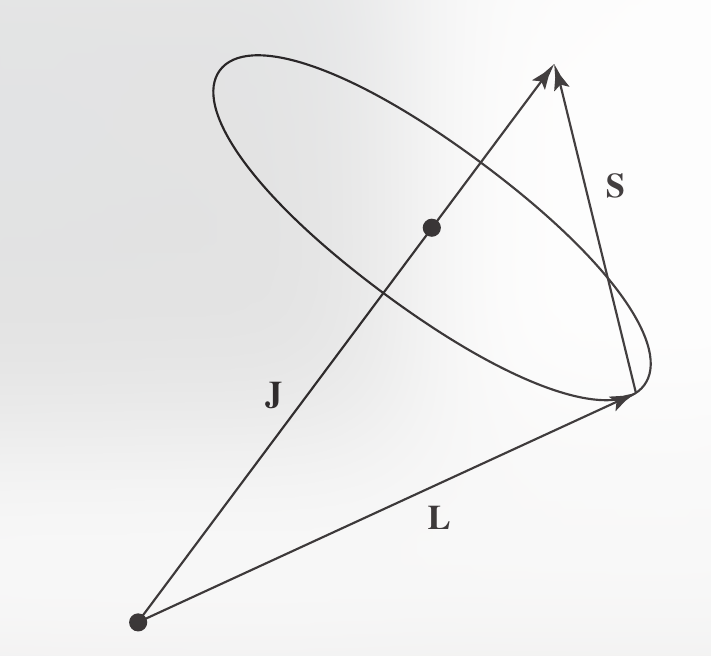
\includegraphics[width=0.3\textwidth]{L17_1.png}
  \caption{In the presence of spin-orbit coupling, $\vec{L}$ and $\vec{S}$ are separately 
  conserved; they precess about the fixed total angular momentum $\vec{J}$}.
\end{figure}
since $j$ and $m_j$ are "good" quantum numbers for a given eigenstate of 
the system under $\hat{H}_\text{Bohr} + \hat{H}_\text{rel} + \hat{H}_\text{SO}$, then the total 
momentum $\big|\vec{J}\big|$ and its direction, so $\vec{J}$ is fixed, and since $l$ is also 
a "good" quantum number, $\big|\vec{L}\big|$ is fixed, but as $m_l$ is not a "good" quantum number,
its direction can precess. Similarly, $s$ is a "good" quantum number as $\big|\vec{S}\big| = 1/2$,
but its direction is indeterminate as $m_s$ is NOT a good quantum number.\\

For a given state $\big|n\,l\,j\,m_j\,s\big>$, the magnitude and direction of $\big|\vec{J}\big|$
is fixed, whereas $\big|\vec{L}\big|$ and $\big|\vec{S}\big|$ are fixed, but their directions 
can vary. However on average
\[
  \big<\vec{S}\big>^2_\text{avg} = \frac{\big<\vec{S}\cdot \vec{J}\big>}{\big<\vec{J}\big>}
\]
In other words, after averaging $\vec{S}$ over a given cycle around $\vec{J}$, the components of 
$\vec{S}$ perpendicular to $\vec{J}$ cancel, and only the components of $\vec{S}$ parallel to 
$\vec{J}$, i.e. $\frac{\vec{S}\cdot\vec{J}}{\big|\vec{J}\big|}$, remain.\\
Similarly 
\begin{align*}
  \vec{L} &= \vec{J}-\vec{S}\\
  L^2 &= \left(\vec{J}-\vec{S}\right)^2 = J^2 - 2\vec{J}\cdot\vec{S} + \vec{S}\\
  \Rightarrow \vec{J}\cdot\vec{S} &= \frac{J^2-L^2+S^2}{2}
\end{align*}
Time averaged $\vec{S}$
\begin{align*}
  \big<\vec{S}\big>_{avg} &\approx \Bigg<\frac{\vec{S}\cdot\vec{J}}{J^2}\vec{J}\Bigg>\\
                          &= \Bigg<\frac{J^2 - L^2 + S^2}{2J^2}\vec{J}\Bigg>
\end{align*}
\begin{align*}
  \big<n, l, s, j, m_j\big|\hat{H}_\text{Zeeman}\big|n, l, s, j, m_j\big> 
  &\cong  \frac{e\,B_{ext}}{2m}\Big<n, l, s, j, m_j\Big|\left(\vec{J}+\frac{J^2-L^2+S^2}{2J^2}
  \vec{J}\right)\cdot\hat{k}\Big|n, l, s, j, m_j\Big>\\
  & \approx \frac{e\,B_{ext}}{2m}\Big<n, l, s, j, m_j\Big|J_z+\frac{J^2-L^2+S^2}{2J^2}
  J_z\Big|n, l, s, j, m_j\Big>\\
  &=\frac{e\,B_{ext}}{2m}\big<J_z\big>\left(1 +\frac{\big<J^2\big>-\big<L^2\big>+
  \big<S^2\big>}{2\big<J^2\big>} \right)\\
  & = \frac{e\,B_{ext}}{2m}\hbar m_j\left(1 +\hbar^2\frac{j(j+1) -l(l+1)+3/4 }{2\hbar^2
  (j(j+1))}\right)\\
  & = \underbrace{\frac{e\,\hbar}{2m}}_{\mu_B}B_{ext}m_j\underbrace{\left(1 + \frac{j(j+1)
  -l(l+1)+3/4}{2j(j+1)}\right)}_{g_J}
\end{align*}
\begin{align*}
  \big<J_z\big> &= \hbar m_j\\
  \big<J^2\big> &= \hbar^2 j(j+1)\\
  \big<L^2\big> &= \hbar^2 l(l+1)\\
  \big<S^2\big> &= \hbar^2 3/4
\end{align*}
\[
\boxed{\mu_B = \frac{e\hbar}{2m}\quad \text{The Bohr Magnetron}}
\]
\[
\boxed{g_J = 1 + \frac{j(j+1) - l(l+1) + 3/4}{2j(j+1)}\quad\text{The Landé g-factor (for an e)}}
\]
\[
  \Rightarrow \big<\hat{H}_{Zeeman}\big> = \mu_B g_J\,B_{ext}m_j \approx \tilde{E}^{(1)}_{Zeeman}
\]
\begin{align*}
  \mu_B &\approx 5.788\times 10^{-5}\,eV/T\\
        &= \frac{1}{2}\quad\text{in atomic units} 
\end{align*}
for $B_{ext}\sim 10T \rightarrow \mu_B\,B_{ext} \sim 0.5788\,MeV$\\
\\
\[
  B_{ext} \ll 12.5\,T\quad \text{in the Weak Zeeman Regime}
\]
%%%%%%%%%%%%%%%%%%%%%%%%%%%%%%%%%%%%%%%%%%%%%%%%%%%%%%%%%%%%%%%%%%%%%%%%%%%%%%%%%%%%%%%%%%%%%%%
%%%%%%%%%%%%%%%%%%%%%%%%%%%%%%%%%%%%%%%%%%%%%%%%%%%%%%%%%%%%%%%%%%%%%%%%%%%%%%%%%%%%%%%%%%%%%%%
%%%%%%%%%%%%%%%%%%%%%%%%%%%%%%%%%%%%%%%%%%%%%%%%%%%%%%%%%%%%%%%%%%%%%%%%%%%%%%%%%%%%%%%%%%%%%%%
%%%%%%%%%%%%%%%%%%%%%%%%%%%%%%%%%%%%%%%%%%%%%%%%%%%%%%%%%%%%%%%%%%%%%%%%%%%%%%%%%%%%%%%%%%%%%%%
\newpage
\section{Lecture 18}
June 05, 2023\\
\\
\[
  \hat{H}_{Zeeman} = -\vec{\mu}_{tot}\cdot \vec{B}_{ind} =
  \frac{e\,B_{ind}}{2m\hbar}(\vec{L}+2\vec{S})\cdot \\at{k}
\]
\textbf{Weak Zeeman Regime}
\[
  B_{ind} \ll B_{SO} \sim 12.7T
\]
\[
  \big<n, l, s, j, m_j\big|\hat{H}_{Zeeman}\big|n, l, s, j, m_j\big>
\]
are eigenstates of $\hat{H}_{Bohr}, \hat{H}_{rel}, \hat{H}_{SO}$.
\[
  E_{Zeeman}^{(1)} \approx \frac{e\hbar}{2m}\left(1+\frac{j(j+1)-l(l+1)+s(s+1)}{2j(j+1)}\right)
  B_{ind}\,m_j = \mu_B\,g_L B_{ind}\,m_j
\]
\subsection{Strong Zeeman Regime}
$B_{ind}\gg B_{SO}\sim 12.5T$\\
\\
In this case we will work in the prefered basis of the Zeeman hamiltonian, using the eigenstates
of the Zeeman Hamiltonian $\hat{H}$.
\[
  \big<H_{Zeeman}\big> = \frac{e\,B_{ind}}{2m}\Big<L_z + 2S_z\Big> = \frac{e\,B_{ind}}{2m}
  \left(\hbar\,m_l + \hbar\,m_s \right)
\]
so $\big|n, l, s, m_l, m_j \big>$ are eigenstates of $\hat{H}_{Zeeman}, \hat{H}_{Bohr}, \hat{H}_
{rel}$ but not $\hat{H}_{SO}$.
\begin{align*}
  E_{Zeeman} &= \mu_B\,B_{ind}(m_l + 2m_s)\\
  E_{rel}^{(1)} &= \frac{-E_1^2}{2mc^2}\frac{1}{n^4}\left[\frac{4n}{l+1/2} - 3\right]\qquad\parbox
  {0.26\textwidth}{This is the same for both basis $\big|n, l, s, j, m_j\big>$ and $\big|n, l, 
  s, m_l, m_s\big>$}\\
  \hat{H}_{SO} &= \left(\frac{e^2}{8\pi\epsilon_0}\right)\frac{1}{m^2 c^2}\frac{\vec{S}\cdot
  \vec{L}}{r^3}
\end{align*}
\[
  \vec{S}\cdot\vec{L} = S_xL_x + S_yL_y + S_zL_z 
\]
\textbf{Idea:} Evaluate the expectation value of $\big<\hat{H}_{SO}\big>$ using $\big|n, l, s, 
m_l, m_s\big>$ as eigenstates. This permits the use of nondegenerate perturbation theory. 
\begin{align*}
  E_{SO}^{(1)} &=\big<n, l, s, m_l, m_s\big|\hat{H}_{SO}\big|n, l, s, m_l, m_s\big> = 
  \frac{e^2}{8\pi\epsilon_0}\frac{1}{m^2c^2}\Big<n, l, s, m_l, m_s\Big|\frac{\vec{L}\cdot
  \vec{S}}{r^3}\Big|n, l, s, m_l, m_s\Big>\\
               &= \frac{e^2}{8\pi\epsilon_0}\frac{1}{m^2c^2}\Big<n, l, s, m_l, m_s
               \Big|\frac{1}{r^3}\Big|n, l, s, m_l, m_s\Big>\left(\big<L_x\big>\big<S_x\big>
               + \big<L_y\big>\big<S_y\big>+\big<L_z\big>\big<L_z\big>\right) 
\end{align*}
\[
  \big<n, \ell, s, m_j, m_s\big|L_{x,y}\big|n, \ell, s, m_\ell, m_s\big> = 0, \qquad
  \big<n, \ell, s, m_j, m_s\big|L_z\big|n, \ell, s, m_\ell, m_s\big> = \hbar m_\ell
\]
\[
  \big<n, \ell, s, m_j, m_s\big|S_{x,y}\big|n, \ell, s, m_\ell, m_s\big> = 0, \qquad
  \big<n, \ell, s, m_j, m_s\big|S_z\big|n, \ell, s, m_\ell, m_s\big> = \hbar m_s
\]
\begin{align*}
&= \frac{e^2}{8\pi\epsilon_0}\frac{1}{m^2c^2}\frac{(\hbar\,m_\ell)(\hbar\,m_s)}{\ell(\ell+1/2)
(\ell+1)n^3a_0^3}\qquad \qquad \qquad \qquad \qquad \qquad \qquad\qquad\qquad\qquad\\
&= \frac{e^2}{8\pi\epsilon_0}\frac{\hbar^2\,m_\ell\,m_s}{m^2c^2n^3\,\ell(\ell+1/2)}
\frac{1}{(\ell+1)a_0^3}
\end{align*}
\[
  \left(\frac{1}{a_0^3}\right) = \left(\frac{m\,e^2}{4\pi\,\epsilon_0\hbar^2}\right)^3, \quad 
  E_1 = \frac{-m\,e^4}{2(4\pi\epsilon_0)^2\hbar^2}
\]
\begin{align*}
&= \frac{e^2\,\hbar^2}{8\pi \epsilon_0\,m^2\,c^2}\left(\frac{m\,e^2}{4\pi\,
\epsilon_0\hbar^2}\right)^3\frac{m_\ell\,m_s}{n^3\,\ell(\ell+1/2)(\ell+1)}\qquad\qquad\qquad\qquad
\qquad\qquad\qquad\quad\\
&= \frac{1}{2}\left(\frac{e^4}{(4\pi\epsilon_0)^2}\right)^2\frac{m^2}{\hbar^4m\,c^2}\frac{n}{n^4}
\frac{m_\ell\,m_s}{\ell(\ell+1/2)(\ell+1)}\\
&= \left[\frac{1}{2}\frac{e^4\,m}{(4\pi\epsilon_0)^2\hbar^2}\right]^2\frac{2}{m\,c^2}\frac{n}
{n^4}\frac{m_\ell\,m_s}{\ell(\ell+1/2)(\ell+1)}\\
&= \frac{2E_n^2}{m\,c^2}\frac{n\,m_\ell\,m_s}{\ell(\ell+1/2)(\ell+1)} = E_{SO}^{(1)}
\end{align*}
\begin{align*}
  E_{fs}^{(1)} &= E_{SO}^{(1)}+E_{rel}^{(1)} = \frac{E_n^2}{m\,c^2}\left[\frac{2\,n\,m_\ell\,
  m_s}{\ell(\ell+1/2)(\ell+1)} + \frac{3}{2}-\frac{2\,n}{\ell+1/2}\right]\\
               &= \frac{E_n^2}{m\,c^2}\left[\frac{3}{2} - \frac{2\,n[\ell(\ell + 1)-m_\ell\,m_s]}
               {\ell(\ell+1/2)(\ell+1)}\right]\\
               &= \frac{2\,E_1^2}{m\,c^2\,n^2}\left[\frac{3}{4\,n}-\frac{\ell(\ell+1) - 
               m_\ell\,m_s}{\ell(\ell+1/2)(\ell+1)}\right]\\
               &= \frac{-2\,E_1}{m\,c^2}\left(\frac{-\alpha^2\,m\,c^2}{2}\right)\frac{1}{n^3}
               \left[\frac{3}{4\,n}-\frac{\ell(\ell+1)-m_\ell\,m_s}{\ell(\ell+1/2)(\ell+1)}\right]\\
               &= \frac{E_1\,\alpha^2}{n^3}\left[\frac{3}{4\,n}-\frac{\ell(\ell+1)
               -m_\ell\,m_s}{\ell(\ell+1/2)(\ell+1)} \right]\\
      E_{\text{S\,Z}}&= \frac{E_1}{n^2}\left[1\right]
\end{align*}






 








%%%%%%%%%%%%%%%%%%%%%%%%%%%%%%%%%%%%%%%%%%%%%%%%%%%%%%%%%%%%%%%%%%%%%%%%%%%%%%%%%%%%%%%%%%%%%%%%%
%%%%%%%%%%%%%%%%%%%%%%%%%%%%%%%%%%%%%%%%%%%%%%%%%%%%%%%%%%%%%%%%%%%%%%%%%%%%%%%%%%%%%%%%%%%%%%%%%
%%%%%%%%%%%%%%%%%%%%%%%%%%%%%%%%%%%%%%%%%%%%%%%%%%%%%%%%%%%%%%%%%%%%%%%%%%%%%%%%%%%%%%%%%%%%%%%%%
%%%%%%%%%%%%%%%%%%%%%%%%%%%%%%%%%%%%%%%%%%%%%%%%%%%%%%%%%%%%%%%%%%%%%%%%%%%%%%%%%%%%%%%%%%%%%%%%%
\newpage 
\section{Lecture 19}
June 06, 2023














































%%%%%%%%%%%%%%%%%%%%%%%%%%%%%%%%%%%%%%%%%%%%%%%%%%%%%%%%%%%%%%%%%%%%%%%%%%%%%%%%%%%%%%%%%%%%%%%%%
%%%%%%%%%%%%%%%%%%%%%%%%%%%%%%%%%%%%%%%%%%%%%%%%%%%%%%%%%%%%%%%%%%%%%%%%%%%%%%%%%%%%%%%%%%%%%%%%%
%%%%%%%%%%%%%%%%%%%%%%%%%%%%%%%%%%%%%%%%%%%%%%%%%%%%%%%%%%%%%%%%%%%%%%%%%%%%%%%%%%%%%%%%%%%%%%%%%
%%%%%%%%%%%%%%%%%%%%%%%%%%%%%%%%%%%%%%%%%%%%%%%%%%%%%%%%%%%%%%%%%%%%%%%%%%%%%%%%%%%%%%%%%%%%%%%%%
\newpage
\section{Lecture 20}
June 07, 2023











































%%%%%%%%%%%%%%%%%%%%%%%%%%%%%%%%%%%%%%%%%%%%%%%%%%%%%%%%%%%%%%%%%%%%%%%%%%%%%%%%%%%%%%%%%%%%%%%%%
%%%%%%%%%%%%%%%%%%%%%%%%%%%%%%%%%%%%%%%%%%%%%%%%%%%%%%%%%%%%%%%%%%%%%%%%%%%%%%%%%%%%%%%%%%%%%%%%%
%%%%%%%%%%%%%%%%%%%%%%%%%%%%%%%%%%%%%%%%%%%%%%%%%%%%%%%%%%%%%%%%%%%%%%%%%%%%%%%%%%%%%%%%%%%%%%%%%
%%%%%%%%%%%%%%%%%%%%%%%%%%%%%%%%%%%%%%%%%%%%%%%%%%%%%%%%%%%%%%%%%%%%%%%%%%%%%%%%%%%%%%%%%%%%%%%%%
\newpage
\chapter{Hyperfine Splitting}
\section{Lecture 21}
June 12, 2023\\
\\
\textbf{Assigment 1:} (Due to June 19th)\\
Further problems Chapter 6 (Griffiths  "Introduction to Quantum Mechanics" vol.1) Problems: 6.27
, 6.28, 6.30, 6.33 (Before the exam)\\
\\
\textbf{Midterm exam: }7-10 am June 19th 

\section{Zeeman Effect (Intermediate)}










































%%%%%%%%%%%%%%%%%%%%%%%%%%%%%%%%%%%%%%%%%%%%%%%%%%%%%%%%%%%%%%%%%%%%%%%%%%%%%%%%%%%%%%%%%%%%%%%%
%%%%%%%%%%%%%%%%%%%%%%%%%%%%%%%%%%%%%%%%%%%%%%%%%%%%%%%%%%%%%%%%%%%%%%%%%%%%%%%%%%%%%%%%%%%%%%%%
%%%%%%%%%%%%%%%%%%%%%%%%%%%%%%%%%%%%%%%%%%%%%%%%%%%%%%%%%%%%%%%%%%%%%%%%%%%%%%%%%%%%%%%%%%%%%%%%
%%%%%%%%%%%%%%%%%%%%%%%%%%%%%%%%%%%%%%%%%%%%%%%%%%%%%%%%%%%%%%%%%%%%%%%%%%%%%%%%%%%%%%%%%%%%%%%%
\newpage
\chapter{Variational Principle}
\section{Lecture 22}
June 13, 2023\\
\\
\textbf{Perturbation theory:} Have a known exact solution to an unperturbed hamiltonian 
and add a minor perturbation:
\[
  \big|\big<n'\big|V\big|n \big>\big| \ll \mathcal{E}_n - \mathcal{E}_{n'}
\]
\begin{itemize}
  \item Approximating the "effect" of the exact hamiltonian for the perturbed system
\end{itemize}
\[
  \parbox{0.15\textwidth}{perturbed hamiltonian}\longrightarrow \tilde{H}\sim \tilde{H}_0
  \longleftarrow \parbox{0.15\textwidth}{unperturbed hamiltonian}
\]
\textbf{Variational Principle: } Choose a trial wavefunction $\tilde{\Psi}$ and solve for the 
exact ground state energy if we were in the trial state $\tilde{\Psi}$. By "varying" the trial 
wavefunction we obtain a lowest upper bound on the ground state energy.
\begin{itemize}
  \item Approximating the ground state wavefunction
\end{itemize}
\[
  \parbox{0.2\textwidth}{exact wavefunction in the ground state}\longrightarrow \Psi_{gs} \sim
  \tilde{\Psi}\longleftarrow \parbox{0.2\textwidth}{trial wavefunction}
\]
\subsection{Theorem (Variational Principle)}
For a hamiltonian $\hat{H}$ with ground state energy $E_{gs}$, and any normalised trial
wavefunction $\tilde{\Psi}$, with $\big<\tilde{\Psi}\big|\tilde{\Psi}\big> = 1$
\[
  \big<\tilde{\Psi}\big|\hat{H}\big|\tilde{\Psi} \big> \geq E_{gs}
\]
\textbf{Proof:}\\
Let $\{\Psi_n\}$ and $\{\mathcal{E}_n\}$ be the normalised eigenstates and eigenenergies of $H$, 
i.e. 
\[
  \hat{H}\big|\Psi\big> = \mathcal{E}_n\big|\Psi\big>, \quad \text{and}\quad \big<\Psi_n\big|
  \Psi_{n'}\big> = \mathlarger{\delta}_{nn'}
\]
then $\{\Psi_n \}$ form a complete basis which spans the Hilbert space of $\hat{H}$, and 
\[
  \mathbb{1} = \sum_{n}\big|\Psi_n\big>\big<\Psi_n\big|
\]
\[
  \big<\tilde{\Psi}\big|\hat{H}\big|\tilde{\Psi}\big> = \bigg<\tilde{\Psi}\bigg|\left(
  \sum_n \big|\Psi_n\big>\big<\Psi_n\big|\right)\hat{H}\left(\sum_{n'}
  \big|\Psi_{n'}\big>\big<\Psi_{n'}\big| \right)\bigg|\tilde{\Psi}\bigg>
\]
\[
  = \sum_n \big<\tilde{\Psi}\big|\Psi_n \big>\big<\Psi_n\big|\sum_{n'}
  \underbrace{\hat{H}\big|\Psi_{n'}
  \big>}_{\mathcal{E}_{n'}\big|\Psi_{n'}\big>} \big<\Psi_{n'}\big|\tilde{\Psi}\big>
\]
\begin{align*}
 & =\sum_{nn'}\big<\tilde{\Psi}\big|\Psi_n\big>\underbrace{\big<\Psi_{n}\big|\mathcal{E}_{n'}
    \big|\Psi_{n'}
  \big>}_{\mathcal{E}_{n'}\delta_{nn'}} \big<\Psi_{n'}\big|\tilde{\Psi}\big>\\
 &=\sum_{nn'}\big<\tilde{\Psi}\big|\Psi_n \big>\big<\Psi_{n'}\big|\tilde{\Psi} \big>
  \mathcal{E}_{n'}\mathlarger{\delta}_{nn'}\\
 &= \sum_{n}\underbrace{\big|\big<\tilde{\Psi}\big|\Psi_n \big>\big|^2}_{\hat{C}_n \hat{C}_n^*}
 \mathcal{E}_n = \sum_{n}\big|\tilde{C}_n\big|^2\mathcal{E}_n
\end{align*}
where $\tilde{C}_n$ are the coefficients of $\tilde{\Psi}$ in the $\{\Psi_n\}$ basis.\\
\\
Since $\mathcal{E}_n \geq E_{gs}\quad \forall n$, i.e. $E_{gs} = \mathcal{E}_1$
\begin{align*}
  &\geq \sum_{n}\big|\tilde{C}_n\big|^2\mathcal{E}_1\\
  &= \mathcal{E}_1\sum_{n}\big|\tilde{C}_n\big|^2\\
  &= E_{gs}\cancelto{1}{\left(\sum_{n}\big|\tilde{C}_n\big|^2 \right)}
\end{align*}
By the Normalisation condition on $\tilde{\Psi}$
\[
  \sum_n \big|\big<\tilde{\Psi}\big|\Psi_n\big>\big|^2 = \sum_{n}\big|\tilde{C}_n\big|^2 = 1
\]
\[
  \big<\tilde{\Psi}\big|\hat{H}\big|\tilde{\Psi} \big> \geq E_{gs} = \mathcal{E}_1
\]
\subsection{Procedure}
\begin{enumerate}
  \item Normalise our trial wavefunction $\tilde{\Psi}(b_1,\cdots,b_n)\rightarrow
    \text{parameters}$
  \item Calculate $\big<\tilde{\Psi}\big|\hat{T}\big|\tilde{\Psi}\big> = \big<\hat{T}
    (b_1, \cdots,b_n)\big>$
  \item Calculate $\big<\tilde{\Psi}\big|\hat{V}\big|\tilde{\Psi}\big>
    = \big<\hat{V}
    (b_1, \cdots,b_n)\big>$
  \item $\big<\tilde{\Psi}\big|\hat{H}\big|\tilde{\Psi}\big> =
    \big<\hat{T}
    (b_1, \cdots,b_n)\big> + \big<\hat{V}
  (b_1, \cdots,b_n)\big>=\tilde{\mathcal{E}}_{gs}(b_1, \cdots, b_n) \geq E_{gs} $.
  \item Minimise $\tilde{\mathcal{E}}_{gs}(b_1, \cdots, b_n) $ w.r.t. the parameters 
    $\{b_1, \cdots, b_n\}$ to obtain the best estimate for $E_{gs}$ and hence:\\
    Set $\Psi_{gs}$ e.g. set:\\
    \[\frac{\partial \tilde{\mathcal{E}}_{gs}}{\partial b} = 0, \quad \text{to find b that minimises}
    \quad \mathcal{E}_{gs}\,\,\,\left(\frac{\partial^2 \tilde{\mathcal{E}}_{gs}}{\partial b^2}
  >0\right)\]
\end{enumerate}
\textbf{Note: } Steps (1) and (2) only need to be applied once for trial wavefunction,
i.e. you may have "pre-prepared" trial wavefunctions that are normalised and have a known 
$\big<\hat{T}(b_1, \cdots,b_n)\big> $. E.g. The gaussian wavefunction has an analytic $\big<
\hat{T}\big>$.
\subsection{Example: 1D Harmonic Oscillator}
\[
  \hat{H} = \underbrace{\frac{-\hbar^2}{2m}\frac{d^2}{dx^2}}_{\hat{T}(x)}+
  \underbrace{\frac{1}{2}m\omega^2x^2}_{V(x)}
\]
Trial wavefunction:
\[ \tilde{\Psi}(x) = A\,e^{-bx^2}\quad \text{(Gaussian)}  \]
\begin{itemize}
  \item $A$: normalisation constant
  \item $b$: parameter
\end{itemize}
\textbf{Step 1:} normalisation 
\[
  1 = \big<\tilde{\Psi}\big|\tilde{\Psi}\big> = A^2\,\int_{-\infty}^{+\infty} e^{-2bx^2}dx
\]
use: 
\begin{equation}
  \int_{0}^{+\infty} e^{-ax^2} = \frac{1}{2}\sqrt{\frac{\pi}{a}}
\end{equation}
then, 
\begin{align*}
  1 &= A^2\,\sqrt{\frac{\pi}{2b}}\\
  \Aboxed{ A &= \left(\frac{2b}{\pi}\right)^{1/4}}
\end{align*}
\textbf{Step 2 and 3: } get $\big<\hat{T}\big>$ and $\big<\hat{V}\big>$\\
First we need the 1st and 2nd derivatives: 
\begin{align*}
  \frac{d \tilde{\Psi}}{dx} &= A \left(-2bx\,e^{-bx^2}\right)\\
  \frac{d^2 \tilde{\Psi}}{dx^2} &= A\left(4b^2x^2-2b\right)e^{-bx^2}\\
                                &= A(2b)(2bx^2-1)e^{-bx^2}\\
                                &= (4b^2x^2-2b)\tilde{\Psi}(x)
\end{align*}
then, 
\begin{align*}
  \big<\tilde{\Psi}\big|\hat{T}\big|\tilde{\Psi}\big>&= \frac{-\hbar^2}{2m}A^2\int_{-\infty}
  ^{+\infty} e^{-2bx^2}(4b^2x^2-2b)dx\\
  &=\frac{-\hbar^2}{2m}\sqrt{\frac{2b}{\pi}}\left[4b^2\frac{\sqrt{\pi}}{2}\frac{1}{(2b)^{3/2}}
  -2b\sqrt{\frac{\pi}{2b}}\right]\\
  &= \frac{\hbar^2 b}{2m}
\end{align*}
for this integral we've used: 
\begin{equation}
  \begin{aligned}
    \int_{0}^{\infty}e^{-ax^2}x^m dx &= \frac{\Gamma\left(\frac{m+1}{2}\right)}
    {2a^{\frac{m+1}{2}}}\\
&= \frac{\sqrt{\pi}}{a^{\frac{m+1}{2}}}\frac{(m-1)\cdot(m-3)\cdots(1)}{m/2}\\
    \int_{-\infty}^{+\infty} e^{-ax^2}x^2dx &= \frac{\sqrt{\pi}}{2a^{\frac{m+1}{2}}}
  \end{aligned}
\end{equation}
\begin{align*}
  \big<\tilde{\Psi}\big|\hat{V}\big|\tilde{\Psi}\big> &= A^2\int_{-\infty}^{+\infty}
  e^{-2bx^2}\left(\frac{1}{2} m \omega^2x^2\right)dx\\
  &= \sqrt{\frac{2b}{\pi}}\left(\frac{m\omega^2}{2}\right)\frac{\sqrt{\pi}}{2}
  \left(\frac{1}{(2b)^{3/2}}\right)\\
  &= \frac{m\omega^2}{8b}
\end{align*}
\textbf{Step 4:} find $\big<\hat{H}\big> = \big<\hat{T}\big>+\big<\hat{V}\big>$
\[
  \frac{\hbar^2 b}{2m} + \frac{m\omega^2}{8b} = \tilde{\mathcal{E}}_{gs}(b)\qquad
  \parbox{0.3\textwidth}{$b$ is the parameter estimate of the ground state energy.}
\]
\textbf{Step 6:} minimise $\tilde{\mathcal{E}}_{gs}$
\begin{align*}
  \frac{\partial \tilde{\mathcal{E}}_{gs}(b)}{\partial b} &= \frac{\partial}{\partial b}
  \frac{\hbar^2 b}{2m} + \frac{\partial }{\partial b}\frac{m\omega^2}{8b}\\
  &= \frac{\hbar^2}{2m} - \frac{m\omega^2}{8b^2} = 0\\
  b^2 &= \frac{m\omega^2}{8}\left(\frac{2m}{\hbar^2}\right) = \frac{m^2\omega^2}{4\hbar^2}\\
  b_{min} &= \frac{m\omega}{2\hbar}
\end{align*}
Now, we can compute $\tilde{\mathcal{E}}_{gs}(b_{min})$:
\begin{align*}
  \tilde{\mathcal{E}}_{gs}(b_{min})&= \frac{\hbar^2}{2m}\left(\frac{m\omega}{2\hbar}\right)
  + \frac{m\omega^2}{8}\left(\frac{2\hbar}{m\omega}\right)\\
                                   &= \frac{\hbar\omega}{4}+\frac{\hbar\omega}{4}\\
                                   &= \frac{\hbar\omega}{2} = E_{gs}
\end{align*}
\[
  \Rightarrow \boxed{\tilde{\Psi} = \Psi_{gs} = \left(\frac{2b}{\pi}\right)^{1/4} 
  \cdot e^{-\frac{m\omega}{2\hbar}x^2}}
\]
\subsection{Example: $\delta$-function potential}
\[
  \hat{V}(x)= -\alpha\delta (x)
\]
\[
  \hat{H} = \frac{-\hbar^2}{2m}\frac{d^2}{dx^2} - \alpha\delta(x)
\]
Trial wavefunction:
\[
  \tilde{\Psi}(x) = Ae^{-bx^2}
\]
Recall: 
\[
  A = \left(\frac{2b}{\pi}\right)^{1/4}, \qquad \big<\hat{T}\big> = \frac{\hbar^2b}{2m}
\]
So we already have step (1), and (2)\\
\\
\textbf{Step 3:}
\begin{align*}
  \big<\hat{V}\big> &= A^2\int_{-\infty}^{+\infty} e^{-2bx^2}(-\alpha \delta(x))dx\\
                    &= -\alpha \sqrt{\frac{2b}{\pi}}\cancelto{1}{e^{-2b(0)^2}}\\
                    &= -\alpha\sqrt{\frac{2b}{\pi}}
\end{align*}
\textbf{Step 4:}
\[
  \big<\hat{H}\big> = \big<\hat{T}\big>+\big<\hat{V}\big> = 
  \frac{\hbar^2 b}{2m} - \alpha\sqrt{\frac{2b}{\pi}} = \tilde{\mathcal{E}}_{gs}(b)
\]
\textbf{Step 5:}
\begin{align*}
  \frac{\partial \tilde{\mathcal{E}}_{gs}(b)}{\partial b} &= \frac{\hbar^2}{2m} -
  \frac{\alpha}{2}\sqrt{\frac{2}{\pi b}} = 0\\
  \Rightarrow \sqrt{b} &= \frac{\alpha\sqrt{2}}{2\sqrt{\pi}}\frac{2m}{\hbar^2}\\
  \Rightarrow b_{min} &= \frac{2\alpha^2 m^2}{\pi \hbar^4}
\end{align*}
\begin{align*}
  \tilde{\mathcal{E}}_{gs}\left(  \frac{2\alpha^2 m^2}{\pi \hbar^4}\right) 
  &= \frac{\hbar^2}{2m}\left( \frac{2\alpha^2 m^2}{\pi \hbar^4}\right)
  - \alpha\sqrt{\frac{2}{\pi}}\left( \frac{2\alpha^2 m^2}{\pi \hbar^4}\right)^{1/2}\\
  &= \frac{\alpha^2 m}{\pi \hbar^2} - \alpha\sqrt{\frac{2}{\pi}}\sqrt{\frac{2}{\pi}}
  \frac{\alpha m}{\hbar^2}\\
  &= \frac{\alpha^2 m}{\pi \hbar^2}\left(1-2\right) = \frac{-\alpha^2 m}{\pi \hbar^2}
\end{align*}
\[
  E_{gs} = \frac{-\alpha^2 m}{2\hbar^2} < \frac{-\alpha^2 m}{\pi \hbar^2} =
  \tilde{\mathcal{E}}_{gs}
\]
\[
  \frac{-1}{2} < \frac{-1}{\pi} \sim 30\%\,\,\text{error} 
\]
For the 1D SHO, the potential \emph{Localises} the wavefunction around $x =0$, whereas for the
$\delta$-function potential, the localisation of the state around $x=0$ is generally weak (
it only acts @ $x=0$).\\
\\
A gaussian give a poor description of the quasi-free electron under a $\delta$-function potential.\\
\\
A free-electron (plane-wave) description might yield better results.
%%%%%%%%%%%%%%%%%%%%%%%%%%%%%%%%%%%%%%%%%%%%%%%%%%%%%%%%%%%%%%%%%%%%%%%%%%%%%%%%%%%%%%%%%%%%%%%%%
%%%%%%%%%%%%%%%%%%%%%%%%%%%%%%%%%%%%%%%%%%%%%%%%%%%%%%%%%%%%%%%%%%%%%%%%%%%%%%%%%%%%%%%%%%%%%%%%%
%%%%%%%%%%%%%%%%%%%%%%%%%%%%%%%%%%%%%%%%%%%%%%%%%%%%%%%%%%%%%%%%%%%%%%%%%%%%%%%%%%%%%%%%%%%%%%%%%
%%%%%%%%%%%%%%%%%%%%%%%%%%%%%%%%%%%%%%%%%%%%%%%%%%%%%%%%%%%%%%%%%%%%%%%%%%%%%%%%%%%%%%%%%%%%%%%%%
\newpage
\section{Lecture 23}
June 14, 2023\\
\\
Choose a trial wavefunction $\tilde{\Psi}$ and minimise $\big<\tilde{\Psi}\big|\hat{H}\tilde{
\big|\Psi}\big> = \tilde{\mathcal{E}}_{gs} \geq E_{gs}$ where $\big<\tilde{\Psi}\big|\tilde
{\Psi}\big> = 1$, but $\tilde{\Psi}$ should be a piecewise continuous, but may have discontinuities 
or be continuous with discontinuities in the derivatives.

\subsection{Example: 1D Square Well}
\begin{wrapfigure}{l}{0.4\textwidth}
  \begin{center}
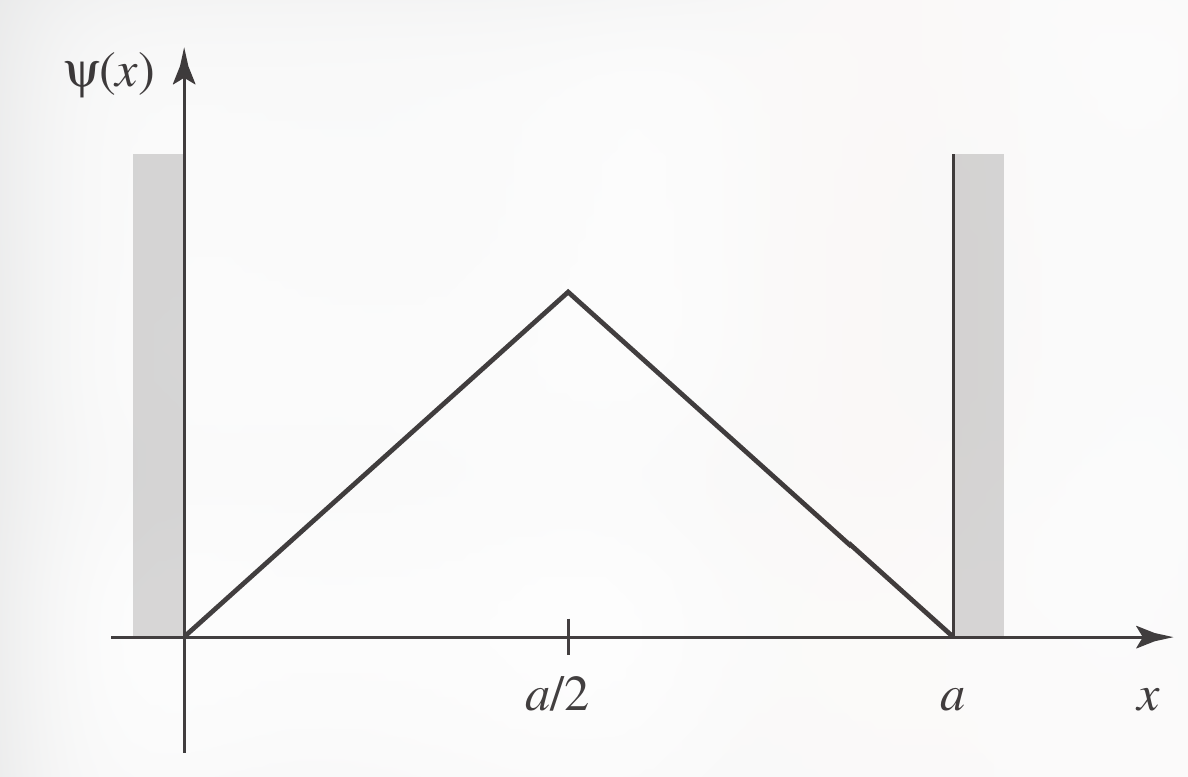
\includegraphics[width=0.35\textwidth]{L23_1.pdf}
  \end{center}
  \caption{Triagular wave function}
\end{wrapfigure}
\
\
\[
V_\infty =
\begin{cases}
  0, & \quad 0 \leq x \leq L\\
  \infty, & \quad \text{otherwise}
\end{cases}
\]

\[
  \tilde{\Psi} (x) = 
  \begin{cases}
    Ax, & \quad 0\leq x \leq L/2\\
    A(L-x), & \quad L/2 \leq x \leq L\\
    0, & \quad \text{otherwise}
  \end{cases}
\]

Then, the hamiltonian will be 
\[
  \hat{H} = \frac{-\hbar^2}{2m}\frac{d^2}{dx^2} + V_\infty 
\]
As before, we need to follow the given steps to accomplish the exercise.\\
\\
\\
\\
Step 1: 
\begin{align*}
  1 =& \big<\tilde{\Psi}\big|\tilde{\Psi} \big> = \int_{0}^{L}\big|\tilde{\Psi}(x)\big|^2dx\\
  &= A^2 \int_{0}^{L/2} x^2 dx  + A^2\int_{L/2}^{L} (L-x)^2dx\\
  &= A^2 \left[\frac{x^3}{3}\bigg|_{0}^{L/2} + \frac{(L-x)^3}{3}(-1)\bigg|_{L/2}^{L}\right]\\
  &= A^2 \left[\frac{L^3}{24}+\frac{L^3}{24} \right] = A^2 \frac{L^3}{12} = 1
\end{align*}
\[
  \boxed{A = \sqrt{\frac{12}{L^3}}}
\]
Step 2: 
\[
  \frac{d\tilde{\Psi}}{dx} \Longrightarrow \parbox{0.3\textwidth}{We can express $\tilde{\Psi}$
  in terms of Heaviside step functions.}
\]
\[
  \Theta (x) = 
  \begin{cases}
    1, & \quad x>0\\
    0, & \quad x < 0\\
    1/2, & \quad x = 0
  \end{cases}
\]
Then
\[
  \tilde{\Psi}(x) = \underbrace{Ax\Theta(x)}_{0\leq x\leq L/2} + 
  \underbrace{(L-2x)\Theta(x-L/2)}_{L/2\leq x\leq L} - 
  \underbrace{(L-x)\Theta(x-L)}_{x\geq L}
\]
Note: $\frac{d}{dx}\Theta(x) = \delta(x)$

\begin{align*}
  \frac{d}{dx}\tilde{\Psi} &= A\left[\frac{d}{dx}(x\,\Theta(x)) + \frac{d}{dx}((L-2x)\,
  \Theta(x-L/2)) + \frac{d}{dx}((x-L)\Theta(x-L))\right]\\
                           &= A\left[\Theta(x)+x\,\delta(x) - 2\,\Theta(x-L/2)+
                           (L-2x)\right]
\end{align*}

%%%%%%%%%%%%%%%%%%%%%%%%%%%%%%%%%%%%%%%%%%%%%%%%%%%%%%%%%%%%%%%%%%%%%%%%%%%%%%%%%%%%%%%%%%%%%%%%%
%%%%%%%%%%%%%%%%%%%%%%%%%%%%%%%%%%%%%%%%%%%%%%%%%%%%%%%%%%%%%%%%%%%%%%%%%%%%%%%%%%%%%%%%%%%%%%%%%
%%%%%%%%%%%%%%%%%%%%%%%%%%%%%%%%%%%%%%%%%%%%%%%%%%%%%%%%%%%%%%%%%%%%%%%%%%%%%%%%%%%%%%%%%%%%%%%%%
%%%%%%%%%%%%%%%%%%%%%%%%%%%%%%%%%%%%%%%%%%%%%%%%%%%%%%%%%%%%%%%%%%%%%%%%%%%%%%%%%%%%%%%%%%%%%%%%%
\clearpage
\newpage
\section{Lecture 24: Midterm Exam}
June 19, 2023




%%%%%%%%%%%%%%%%%%%%%%%%%%%%%%%%%%%%%%%%%%%%%%%%%%%%%%%%%%%%%%%%%%%%%%%%%%%%%%%%%%%%%%%%%%%%%%%%%
%%%%%%%%%%%%%%%%%%%%%%%%%%%%%%%%%%%%%%%%%%%%%%%%%%%%%%%%%%%%%%%%%%%%%%%%%%%%%%%%%%%%%%%%%%%%%%%%%
%%%%%%%%%%%%%%%%%%%%%%%%%%%%%%%%%%%%%%%%%%%%%%%%%%%%%%%%%%%%%%%%%%%%%%%%%%%%%%%%%%%%%%%%%%%%%%%%%
%%%%%%%%%%%%%%%%%%%%%%%%%%%%%%%%%%%%%%%%%%%%%%%%%%%%%%%%%%%%%%%%%%%%%%%%%%%%%%%%%%%%%%%%%%%%%%%%%
\newpage
\section{Lecture 25}
June 20, 2023





%%%%%%%%%%%%%%%%%%%%%%%%%%%%%%%%%%%%%%%%%%%%%%%%%%%%%%%%%%%%%%%%%%%%%%%%%%%%%%%%%%%%%%%%%%%%%%%%%
%%%%%%%%%%%%%%%%%%%%%%%%%%%%%%%%%%%%%%%%%%%%%%%%%%%%%%%%%%%%%%%%%%%%%%%%%%%%%%%%%%%%%%%%%%%%%%%%%
%%%%%%%%%%%%%%%%%%%%%%%%%%%%%%%%%%%%%%%%%%%%%%%%%%%%%%%%%%%%%%%%%%%%%%%%%%%%%%%%%%%%%%%%%%%%%%%%%
%%%%%%%%%%%%%%%%%%%%%%%%%%%%%%%%%%%%%%%%%%%%%%%%%%%%%%%%%%%%%%%%%%%%%%%%%%%%%%%%%%%%%%%%%%%%%%%%%
\newpage
\chapter{Time Dependent Perturbation Theory}
\section{Lecture 25}
July 17, 2023

\subsection{Time Dependent Quantum Mechanics}
Time dependent Schrodinger Eq'n 
\[
  \hat{H}\Psi(\vec{r}, t) = i\,\hbar\frac{\partial \Psi}{\partial t} 
\]
Let $E$ be the eigenvalue of $\hat{H}$ i.e., the energy, so that 
\[
  \hat{H}\Psi(\vec{r}, t) = E\Psi(\vec{r}, t) = i\,\hbar\frac{\partial \Psi}{\partial t}
\]
Assume $\Psi(\vec{t}, r)$ is separable, i.e., $\Psi(\vec{r}, t) = \psi(\vec{r})\varphi(t)$
\[
  E\cancel{\psi(\vec{r})}\varphi(t) = i\hbar\cancel{\psi(\vec{r})}\frac{\partial \varphi}{\partial t}
\]
\[
  \varphi'(t) = \frac{-i}{\hbar}\varphi(t) \Rightarrow \varphi(t) = e^{-\frac{iE}{\hbar}t}
\]
\[
  \Rightarrow \Psi(\vec{r}, t) = \psi(\vec{r})\,e^{-\frac{iE}{\hbar}t}
\]
where $\hat{H}\psi(\vec{r}) = E\psi(\vec{r})$.\\
\\
if we want to consider transitions, excitations, and quantum dynamics, we can express the time 
dependent state $\Psi(\vec{r}, t)$ as a time dependent linear combination of eigenstates of the 
system. 
\[
  \Psi(\vec{t}, r) = \sum_n C_n(t)\,e^{-\frac{i\mathcal{E}_n}{\hbar}t}
\]
where 
\begin{align*}
  \hat{H}\big|\psi_n\big> &= \mathcal{E}_n\big|\psi_n\big>\\
  \big<\psi_n\big|\psi_{n'}\big> &= \delta_{n'n}\\
  \big<\Psi\big|\psi_n\big> &= C_n(t)\,e^{-\frac{i}{\hbar}\mathcal{E}_n\,t}
\end{align*}
\begin{align*}
  \big<\psi\big|\psi\big> &= 1 \qquad \text{(normalisation)}\\
  \big<\Psi\underbrace{\big|\sum_n\big|\psi_n\big>\big<\psi_n\big|}_{\mathbb{1}}&\big|\Psi\big> \qquad
  \text{(Completeness)}
\end{align*}
\[
  = \sum_{nn'n''}C^{\dagger}_n\,e^{\frac{i}{\hbar}\mathcal{E}_n\,t}\big<\psi_n\big|\psi_{n'}\big>
  \big<\psi_n'\big|C_{n''}\,e^{-\frac{i}{\hbar}\mathcal{E}_{n''}\,t}\big|\psi_{n''}\big>
\]
\[
  \sum_n C^\dagger_n C_n e^{\frac{i}{\hbar}(\mathcal{E}_n - \mathcal{E}_n)t} 
  = \sum_n \big|C_n\big|^2 = 1 
\]
A time dependent perturbation will lead to time dependent coefficients $C_n(t)$, but will still
be spanned by the eigenbasis $e^{-\frac{i}{\hbar}\mathcal{E}t}\big|\psi_n\big>$.\\
\\
Suppose 
\[
  \hat{H}(\vec{r}, t) = \hat{H}_0(\vec{r}) + V(t)
\]
\begin{align*}
  \hat{H}(\vec{r}, t)\Psi(\vec{r}, t) &= i\hbar \frac{\partial \Psi}{\partial t}\\
  \left(\hat{H}_0(\vec{r}) + V(t)\right)\sum_n C_n(t)\,e^{-\frac{i}{\hbar}\mathcal{E}_n t}
  \psi_n(\vec{r}) &= i\hbar\frac{\partial}{\partial t}\sum_{n'} \dot{C}_n(t) 
  \,e^{-\frac{i}{\hbar}\mathcal{E}_{n'}t}\psi_{n'}(\vec{r})\\
  \sum_n C_n(t)e^{-\frac{i}{\hbar}\mathcal{E}_{n}t}\hat{H}_0(\vec{r})\psi_n(\vec{r}) + V(t)
  C_n(t)e^{-\frac{i}{\hbar}\mathcal{E}_{n}t}\psi_n(\vec{r}) &= i\hbar \sum_{n'}
  \left(\dot{C}_{n'}(t) - \frac{i}{\hbar}\mathcal{E}_{n'}C_{n'}(t) \right)e^{-\frac{i}{\hbar}
  \mathcal{E}_{n'}t}\psi_{n'}(\vec{r})
\end{align*}
Time Independent Schrodinger Eq'n
\[
  \hat{H}(\vec{r})\psi_n(\vec{r}) = \mathcal{E}_n\psi_n(\vec{r})
\]
Therefore 
\begin{align*}
  \sum_n\left(\mathcal{E}_n + V(t) \right)C_n(t) e^{-\frac{i}{\hbar}\mathcal{E}_n\,t}\psi_n{\vec{r}}
  &= \sum_{n'}\left(i\,\hbar\dot{C}_{n'}(t) + \mathcal{E}_{n'}C_{n'}(t)\right) e^{-\frac{i}{\hbar}
  \mathcal{E}_{n'}t}\psi_{n'}(\vec{r})\\
  \sum_n V(t)C_n(t) e^{-\frac{i}{\hbar}\mathcal{E}_nt}\psi_n(\vec{r}) &= 
  \sum_{n'}i\hbar \,\dot{C}_{n}(t) e^{-\frac{i}{\hbar}\mathcal{E}_n t}\\
  \sum_n\left(V(t)\,C_n(t)- i\hbar\,\dot{C}_n(t)\right)e^{-\frac{i}{\hbar}\mathcal{E}_n t}
  \psi_n(\vec{r})&= 0
\end{align*}
Multiply by $\big<\psi_n'\big|$:
\begin{align*}
  \sum_n \big<\psi_{n'}\big|V(t)\big|\psi_n\big>C_n(t)e^{-\frac{i}{\hbar}\mathcal{E}_n t} 
  &= \sum_n i\hbar\,\dot{C}_n(t)e^{-\frac{i}{\hbar}\mathcal{E}_n t}\cancelto{\delta_{nn'}}{
    \big<\psi_{n'}\big|\psi_n\big>
  }\\
  &= i\hbar\,\dot{C}_{n'}(t)e^{-\frac{i}{\hbar}\mathcal{E}_{n'} t}
\end{align*}
\[\boxed{
  \dot{C}_n(t) =-\frac{i}{\hbar}\sum_n C_n(t)\underbrace{e^{-\frac{i}{\hbar}\left(\mathcal{E}
        _{n'}-
  \mathcal{E}_n\right)t}}_{\omega_{nn'}}\underbrace{\big<\psi_{n'}\big|V(t)\big|\psi_n\big>}_
  {\scriptsize  \begin{split}
    &\text{matrix elements of}\\
    &\text{the perturbation.}\end{split}}
}\]
\subsection{For a two-level system}
\begin{align*}
  \dot{C}_a (t) &= -\frac{i}{\hbar}\left(C_a(t)\big<\psi_a\big|\hat{V}(t)\big|\psi_a\big>
  + C_b(t) e^{-i\omega_0 t}\big<\psi_a\big|\hat{V}(t)\big|\psi_b\big>\right)\\
    \dot{C}_b(t) &= -\frac{i}{\hbar} \left(C_a(t)e^{i\omega_0 t}\big<\psi_b\big|\hat{V}(t)
  \big|\psi_a\big> + C_b (t)\big<\psi_b\big|\hat{V}(t)\big|\psi_b\big>\right)
    \end{align*}
For the special case $\big<\psi_n\big|\hat{V}(t)\big|\psi_n\big> = 0$, where the perturbation 
transitions between eigenstates which is often the case. 
\begin{align*}
  \dot{C}_a(t) &= -\frac{i}{\hbar}C_b(t)\,e^{-i\omega_0 t}\big<\psi_a\big|\hat{V}(t)\big|\psi_b
  \big>\\
\dot{C}_b(t) &= -\frac{i}{\hbar}C_a(t)\,e^{i\omega_0 t}\big<\psi_b\big|\hat{V}(t)\big|\psi_a
  \big>
\end{align*}
\[\boxed{
    \dot{C}_{n'}(t) = -\frac{i}{\hbar}\sum_n C_n(t)e^{i\omega_{nn'}t}\big<\psi_{n'}\big|
    \hat{V}(t)\big|\psi_n\big> 
}\]
\subsection{Example}
\[
  \vec{E}(\vec{r}, t) = E(t)\hat{k}, \qquad \hat{V}(t) = -e\mathcal{E}z\Theta(t)\quad\text{(
    Heaviside step function
  )}
\]
A constant electric field in the $\hat{k}$ direction which turns on after $t=0$. For a hydrogen 
atom, calculate the matrix elements:
\begin{align*}
  \mathlarger{\varphi}_{100}(r) &= \frac{1}{\sqrt{\pi a_0^3}}e^{-r/a_0}\\
  \mathlarger{\varphi}_{200}(r) &= \frac{(2-r/a_0)}{4\sqrt{2\pi a_0^3}}
  e^{-r/2a_0}\\
  \mathlarger{\varphi}_{210}(r, \phi) &= \frac{r\cos\phi}{4 a_0\sqrt{2\pi a_0^3}}e^{-r/2a_0}\\
  \mathlarger{\varphi}_{21\pm 1}(r,\theta, \phi) &= \frac{r\sin\phi}{8 a_0\sqrt{\pi a_0^3}}
  e^{-r/2a_0}e^{\pm i\theta}
\end{align*}
\begin{align*}
  \big<\mathlarger{\varphi}_{100}\big|\hat{V}\big|\mathlarger{\varphi}_{100}\big> &= 
  \int \underbrace{\big|\mathlarger{\varphi}_{100}(r)\big|^2}_\text{even}
  \underbrace{\left(e\mathcal{E}z\right)}_\text{odd}dr d\Omega = 0\\
\big<\mathlarger{\varphi}_{100}\big|\hat{V}\big|\mathlarger{\varphi}_{200}\big> &=
\int \underbrace{\mathlarger{\varphi}_{100}(r)\mathlarger{\varphi}_{200}(r)}_\text{even in z}
\underbrace{\left(-e\mathcal{E}z\right)}_\text{odd in z}drd\Omega\\
\big<\mathlarger{\varphi}_{100}\big|\hat{V}\big|\mathlarger{\varphi}_{210}\big> &\neq 0\\
\big<\mathlarger{\varphi}_{100}\big|\hat{V}\big|\mathlarger{\varphi}_{210}\big>
&=\int\int\int \frac{e^{-3r/2a_0^4}}{4\pi a_0} r\cos\phi\left(-e\mathcal{E}r\cos\phi\right)r^2
\sin\phi dr\,d\theta\,d\phi\\
&= -\frac{e\mathcal{E}}{4\pi a_0^4}\int_{0}^{2\pi}d\theta\int_{0}^{\pi}\cos^2\phi\sin\phi\,d\phi
\int_{0}^{\infty}e^{-\frac{3}{2} \frac{r}{a_0}}r^4\,dr\\
&= -\frac{e\mathcal{E}}{2a_0^4}\left(\frac{-\cos^3\phi}{3}\right)\bigg|_{0}^{\pi} \frac{
  \cancelto{4!}{ \Gamma(4+1)
}}{(3/2a_0)^{5}}\\
&= -e\mathcal{E}a_0\frac{2^8}{3^5} = -\frac{2^8}{3^5}e\mathcal{E}a_0
\end{align*}
\newpage 
%%%%%%%%%%%%%%%%%%%%%%%%%%%%%%%%%%%%%%%%%%%%%%%%%%%%%%%%%%%%%%%%%%%%%%%%%%%%%%%%%%%%%%%%%%%%%%%%%
%%%%%%%%%%%%%%%%%%%%%%%%%%%%%%%%%%%%%%%%%%%%%%%%%%%%%%%%%%%%%%%%%%%%%%%%%%%%%%%%%%%%%%%%%%%%%%%%%
%%%%%%%%%%%%%%%%%%%%%%%%%%%%%%%%%%%%%%%%%%%%%%%%%%%%%%%%%%%%%%%%%%%%%%%%%%%%%%%%%%%%%%%%%%%%%%%%%
%%%%%%%%%%%%%%%%%%%%%%%%%%%%%%%%%%%%%%%%%%%%%%%%%%%%%%%%%%%%%%%%%%%%%%%%%%%%%%%%%%%%%%%%%%%%%%%%%
\section{Lecture 40}
July 18, 2023
\subsection{Example}
$H$ atom in
\[
  V(z) = -e\mathcal{E} \Theta (t), \qquad \Theta(t) = \begin{cases}
    1,&\quad t>0\\
    0,&\quad t<0\\
    1/2&\quad t=0
  \end{cases}
\]
From the previous class, we know that
\[
\big<\mathlarger{\varphi}_{100}\big|\hat{V}(z)\big|\mathlarger{\varphi}_{210}\big> = 
-\frac{e\mathcal{E}a_02^8}{3^5}
\]
and 
\[
  \dot{C}_n(t) =-\frac{i}{\hbar} \sum_{n'}C_{n'}(t)\,e^{i\omega_{nn'}t}
  \big<\psi_n\big|\hat{V}\big|\psi_{n'}\big>, \qquad \omega_{nn'} \equiv \frac{\mathcal{E}_n-
  \mathcal{E}_{n'}}{\hbar}
\]
\begin{align*}
  \Rightarrow \dot{C}_{210}(t)&= -\frac{i}{\hbar}C_{100}(t)\,e^{i\frac{E_2-E_1}{\hbar}t}
  \left(-\frac{2^8}{3^5}e\mathcal{E}a_0\right)\\
  \dot{C}_{210}(t) &= \frac{i}{\hbar}C_{100}(t)e^{-i\frac{3}{4}\frac{E_1}{\hbar} t}
  \left(\frac{2^8}{3^5}e\mathcal{E}a_0 \right)\\
                   &= \frac{2^8}{3^5}\frac{i}{\hbar} e\mathcal{E}a_0 C_{100}
                   (t)\,e^{-\frac{i3}{4}\frac{E_1}{\hbar}t}
\end{align*}
Assume @ $t=0$ $C_{100}(0)=1$ and $C_{210}(0) = 0$ (initially in the ground state)
\begin{align*}
  \frac{dC_{210}}{dt} &= \frac{2^8}{3^5}\frac{i}{\hbar} e\mathcal{E}a_0e^{-\frac{i3}{4}
  \frac{E_1}{\hbar}t}C_{100}(t), \quad \big|C_{100}(t)\big|^2+\big|C_{210}(t)\big|^2 = 1\\
                      &\Rightarrow C_{100}(t) = \sqrt{1-\big|C_{210}(t)\big|^2}\\
    C_{210}(t) &= \frac{2^8}{3^5}\frac{i}{\hbar}e\,\mathcal{E}a_0\int_{0}^{t}
                      e^{-\frac{i3}{4}\frac{E_1}{\hbar}t}
\end{align*}
\subsection{Example}
Solve
\begin{align*}
  \dot{C}_a (t)&= -\frac{i}{\hbar}e^{-i\omega_0t}C_b(t)\big<\psi_a\big|\hat{V}\big|\psi_b\big>\\
\dot{C}_b (t)&= -\frac{i}{\hbar}e^{i\omega_0t}C_a(t)\big<\psi_b\big|\hat{V}\big|\psi_a\big>
\end{align*}
where $\hat{V}(\vec{r})$ (time independent) and $C_a(0) = 1, C_b(0) = 0$.\\
\\
Differentiating:
\begin{align*}
  \ddot{C}_a(t) &= -\frac{i}{\hbar}e^{-i\omega_0t}\big<\psi_a\big|\hat{V}\big|\psi_b\big>
  \left(\dot{C}_b(t) - i\omega_0C_b(t)\right)\\
  \therefore \ddot{C}_b(t) &= -\frac{i}{\hbar}e^{i\omega_0t}\big<\psi_b\big|\hat{V}\big|\psi_a\big>
  \left(\dot{C}_a(t) + i\omega_0C_a(t)\right)\quad (*)
\end{align*}
We want to solve for $C_b(t)$, so we need an ODE in $C_b(t)$.\\
\\
Subtitute
\begin{align*}
  \dot{C}_a(t) &=-\frac{i}{\hbar}e^{-i\omega_0t}C_b(t)\big<\psi_a\big|\hat{V}\big|\psi_b\big>\\
  C_a(t) &= \frac{i\hbar \dot{C}_b (t)e^{-i\omega_0 t}}{\big<\psi_b\big|\hat{V}\big|\psi_a\big>}
\end{align*}
into ($*$)
\begin{align*}
  \ddot{C}_b(t) &= \frac{i}{\hbar}e^{i\omega_0 t}\big<\psi_b\big|\hat{V}\big|\psi_a\big>
  \left[\frac{i}{\hbar}e^{-i\omega_0 t}C_b(t)\big<\psi_a\big|\hat{V}\big|\psi_b\big>
   + i\,\omega_0(i\hbar)\frac{\dot{C}_b(t)e^{-i\omega_0 t}}{\big<\psi_b\big|\hat{V}
\big|\psi_a\big>} \right]\\
  \ddot{C}_b(t) &= -\frac{1}{\hbar^2}C_b(t)\big|\big<\psi_a\big|\hat{V}\big|\psi_b\big>\big|^2
  + i\omega_0 \dot{C}_b(t)
\end{align*}
\[
  \Rightarrow \ddot{C}_b(t) - i\omega_0 \dot{C}_b(t)+\frac{C_b(t)}{\hbar^2}
  \big|\big<\psi_a\big|\hat{V}\big|\psi_b\big>\big|^2 = 0
\]
A $2^{ND}$ order ODE with constant coefficients.
\[
  C_b(t) \sim A\,e^{\lambda_+ t} + B\,e^{\lambda_-t}
\]
\begin{align*}
  \lambda_\pm &= \frac{i\omega_0}{2}\pm \frac{1}{2}\sqrt{-\omega_0^2 - 4\frac{\big|\big<
  \psi_a\big|\hat{V}\big|\psi_b\big>\big|^2}{\hbar^2}}\\
              &= \frac{i}{2}\left(\omega_0 \pm \sqrt{\omega_0^2 + 4\frac{\big|\big<
              \psi_a\big|\hat{V}\big|\psi_b\big>\big|^2}{\hbar^2}}\right)
\end{align*}
\begin{align*}
  C_b (t) &= A\,\exp\left[\frac{it}{2}\left(\omega_0 + \sqrt{\omega_0^2 + 4\frac{\big|V_{ab}
  \big|^2}{\hbar^2}}\right)\right]
  +  B\,\exp\left[\frac{it}{2}\left(\omega_0 - \sqrt{\omega_0^2 + 4\frac{\big|V_{ab}
  \big|^2}{\hbar^2}}\right)\right]\\
          &= \exp\left(\frac{i\omega_0 t}{2}\right)\left[A\exp\left(\frac{it}{2}\sqrt{\omega_0^2
              +\frac{4\big|V_{ab}|^2}{\hbar^2}}\right)+B\exp\left(-\frac{it}{2}\sqrt{\omega_0^2
              +\frac{4\big|V_{ab}|^2}{\hbar^2}
}\right)\right]\\
 C_b(t)&= \exp\left(\frac{i\omega_0 t}{2}\right)\left[C\cos\left(\sqrt{\frac{\omega_0^2}{4}
        +\frac{\big|V_{ab}|^2}{\hbar^2}}t\right)+D\sin\left(\sqrt{\frac{\omega_0^2}{4}
        +\frac{\big|V_{ab}|^2}{\hbar^2}}t\right) \right]
\end{align*}
But $C_b(0)=0$ (initially in $C_a = 1$) therefore $C=0$ and $D=1$
\begin{align*}
  C_b(t) &= \exp\left(\frac{i\omega_0 t}{2}\right)\sin\left(\sqrt{\frac{\omega_0^2}{4}
        +\frac{\big|V_{ab}|^2}{\hbar^2}}t\right)\\
  C_a(t) &= \exp\left(-\frac{i\omega_0 t}{2}\right)\cos\left(\sqrt{\frac{\omega_0^2}{4}
        +\frac{\big|V_{ab}|^2}{\hbar^2}}t\right)
\end{align*}
Check $\big|C_a(t)\big|^2+ \big|C_b(t)\big|^2 = 1$
\[
 \Rightarrow \cos^2\left(\sqrt{\frac{\omega_0^2}{4}
        +\frac{\big|V_{ab}|^2}{\hbar^2}}t\right)+
        \sin^2\underbrace{\left(\sqrt{\frac{\omega_0^2}{4}
          +\frac{\big|V_{ab}|^2}{\hbar^2}}t\right)}_{\scriptsize \begin{split} & \text{Rabi frequency}\\
&\text{switching between}\\
&\psi_a \& \psi_b \end{split}} = 1 
\]

\begin{align*}
  V(t) = \mathcal{U}\delta(t-t_0),\quad \mathcal{U}_{aa} = \mathcal{U}_{bb}=0,\quad\mathcal{U}_{ab}
  =\mathcal{U}_{ba}^{\dagger} = \alpha,\quad C_a(-\infty) =1, \quad C_b(-\infty) = 0
\end{align*}

\begin{equation*}
 \left.\begin{aligned}
     \dot{C}_a (t) &= -\frac{i}{\hbar}C_b(t)e^{-i\omega_0t}\alpha \delta(t-t_0)\\
     \dot{C}_b (t) &= -\frac{i}{\hbar}C_a(t)e^{i\omega_0t}\alpha^{\dagger}\delta(t-t_0)
       \end{aligned}
 \right\}
 \quad \scriptsize \parbox{0.2\textwidth}{ODE in $C_b$ alone and its derivatives, differentiating
 to obtain a 2nd order ODE in $C_b(t)$}
\end{equation*}
\begin{align*}
  \delta(t-t_0) &= \lim_{\epsilon\to 0} P_\epsilon (t-t_0) = \frac{\Theta(t-t_0+\epsilon/2)
  -\Theta(t-t_0-\epsilon/2)}{\epsilon}\\
                &= \begin{cases}
                  1/\epsilon,&\quad (t-t_0)<\epsilon/2\\
                  0,&\quad \text{otherwise}
                \end{cases}
\end{align*}
\[
  \ddot{C}_b(t)=-\frac{i}{\hbar}e^{i\omega_0 t}\alpha^\dagger \left[
  \dot{C}_a(t)\delta(t-t_0)+ i\omega_0 C_a(t)\delta(t-t_0) + C_a(t)\frac{d}{dt}\delta
(t-t_0)\right]
\]
Let $t_0=0$ wlog, for $t<-\epsilon/2$, $C_a(t) = 1$, $C_b = 0$\\ 
After $t>\epsilon/2$, $C_a(t) = C_a^0$, $C_b(t) = C_b^0$\\
\\
For $\big|t\big|>\epsilon/2$, then $\delta(t-t_0) = 1/\epsilon$, $\frac{d}{dt}\delta(t-t_0) = 0$
\[
  \ddot{C}_b(t) = -\frac{i}{\hbar}e^{i\omega_0 t} \alpha^*\left(\frac{\dot{C}_a(t)}{\epsilon}
  + \frac{i\omega_0 C_a(t)}{\epsilon} \right) 
\]
\begin{align*}
  C_a(t) &= \frac{i\hbar \dot{C}_b(t)e^{-i\omega_0 t}\epsilon}{\alpha^*}\\
  \dot{C}_a(t) &= -\frac{i}{\hbar}C_b(t)e^{-i\omega_0 t}\frac{\alpha}{\epsilon} 
\end{align*}
Therefore 
\[
  \ddot{C}_b (t) = -\frac{i}{\hbar}e^{i\omega_0 t}\left[-\frac{i}{\hbar}e^{-i\omega_0 t}
  C_b(t) \frac{\big|\alpha\big|^2}{\epsilon^2}+ i\omega_0 (i\hbar)e^{-i\omega_0 t}
\dot{C}_b(t)\right]
\]
\[
  \ddot{C}_b(t) + \frac{\big|\alpha\big|^2}{\hbar^2\epsilon^2}C_b(t)-i\omega_0\dot{C}_b(t) = 0
\]
A second order ODE  with constant coefficients.
\[
  \lambda_\pm = \frac{i\omega_0}{2}\pm\sqrt{-\omega_0^2 - \frac{4\big|\alpha\big|^2}{\epsilon^2
  \hbar^2}} = \frac{i}{2}\Bigg(\omega_0 \pm \underbrace{\sqrt{\omega_0^2 +\frac{4\big|\alpha\big|^2}
  {\epsilon^2\hbar^2}}}_{\omega_R}\Bigg)
\]
\begin{align*}
  C_b(t) &= \exp\left(\frac{i\omega_0}{2}t\right)\left[A\exp\left(\frac{i\omega_R}{2}t\right)
  + B\exp\left(-\frac{i\omega_R}{2}t\right)\right]\\
         &= \exp\left(\frac{i\omega_0}{2}t\right)\left[C\cos\left(\frac{\omega_R}{2}t\right)
         +D\sin\left(\frac{\omega_R}{2}t\right)\right]\\
    C_b(-\epsilon/2)&=0 = \exp\left(\frac{-i\omega_0\epsilon}{4}\right)\left[C\cos\left(
    -\frac{\omega_R\epsilon}{4}\right) +D\sin\left(-\frac{\omega_R\epsilon}{4}\right)\right]\\
  C\cos\left(\frac{\omega_R\epsilon}{4}\right) &= D\sin\left(\frac{\omega_R\epsilon}{4}\right)
\end{align*}
\[
  \Rightarrow C = D\tan\left(\frac{\omega_R\epsilon}{4}\right)
\]
\[
  C_b(t) = \exp\left(\frac{i\omega_0 t}{2}\right)D\left[\tan\left(\frac{\omega_R \epsilon}{4}
  \right)\cos\left(\frac{\omega_Rt}{2}\right)+\sin\left(\frac{\omega_R t}{2}\right)\right]
\]
\begin{align*}
  C_a(t) &= \frac{i\hbar}{\alpha^*}\dot{C}_b(t)e^{-i\omega_0 t}\epsilon\\
         &= \frac{i\hbar}{\alpha^*}\epsilon \exp\left(-\frac{i\omega_0 t}{2}\right)D\left[
         \left(\frac{i\omega_0}{2}
       \cos\left(\frac{\omega_R t}{2}\right)- \frac{\omega_R}{2}\sin\left(\frac{\omega_Rt}{2}
     \right)\right)\tan\left(\frac{\omega_R\epsilon}{4}\right)\right.\\
         &+\left. \left(\frac{i\omega_0}{2}\sin\left(\frac{\omega_Rt}{2}\right) +
         \frac{\omega_R}{2}\cos\left(\frac{\omega_R t}{2}\right)\right) \right]\\
  C_a(-\epsilon/2) &= 1 = \frac{i\hbar\epsilon}{\alpha^*}\exp\left(\frac{i\omega_0\epsilon}{4}
  \right)D\left[\left(\frac{i\omega_0}{2}\cos\left(\frac{\omega_R\epsilon}{4}\right)+
  \frac{\omega_R}{2}\sin\left(\frac{\omega_R \epsilon}{4}\right)\right)
\tan\left(\frac{\omega_R\epsilon}{4}\right)\right.\\
                   &\left. + \left(-\frac{i\omega_0}{2}\sin\left(\frac{\omega_R\epsilon}{4}\right)
                   + \frac{\omega_R}{2}\cos\left(\frac{\omega_R\epsilon}{4}\right)\right)\right]\\
    1&= \frac{i\hbar\epsilon}{\alpha^*}\exp\left(\frac{-i\omega_0 \epsilon}{4}\right)D\left[
      \right]
    \end{align*}

Look for the missing examples in the QM 2 book











\end{document}
